% Sam Avis, Durham University Physics department.
% sam.avis@durham.ac.uk or avissam96@gmail.com
% Thesis template


\documentclass[11pt, twoside, openright, a4paper]{report}
% Packages
\usepackage[section]{placeins}
\usepackage[square, numbers, comma, sort&compress]{natbib}
\setcitestyle{numbers,super}
\usepackage{caption}
\captionsetup{font={small}}
\setlength{\parskip}{1em}

%\makeatletter

\newcommand\frontmatter{%
  %\cleardoublepage
  %\@mainmatterfalse
  \pagenumbering{roman}}

\newcommand\mainmatter{%
  \cleardoublepage
%   %\@mainmattertrue
  \pagenumbering{arabic}}

\newcommand\backmatter{%
  \if@openright
  \cleardoublepage
  \else
  \clearpage
  \fi
  % \@mainmatterfalse
}

% \makeatother

% Geometry
\usepackage[a4paper,width=141mm,top=35mm,bottom=35mm,bindingoffset=8mm]{geometry}
% \linespread{1.5}

% Header
\usepackage{fancyhdr}
\pagestyle{fancy}
\fancyhf[lh,rh,ch]{}
\fancyhf[leh]{\leftmark}
\fancyhf[roh]{\rightmark}
\setlength{\headheight}{13.6pt}

% Table of contents
\setcounter{tocdepth}{2}

% Text
\usepackage[utf8]{inputenc}
\usepackage[T1]{fontenc}
\usepackage[doublespacing]{setspace}
\usepackage{siunitx}
\usepackage{xcolor}
% Ticks and crosses
\usepackage{pifont}
\newcommand{\cmark}{\ding{51}}
\newcommand{\xmark}{\ding{55}}

% Lists
\usepackage{enumitem}
\setlist{nosep, before={\parskip=0pt}, after=\vspace{0pt}}%-\docparskip}}

% Maths
\usepackage{bm}
\usepackage{amsmath}
\usepackage{amssymb}
\newcommand{\abs}[1]{\left| #1 \right|}
\newcommand{\grad}{\bm{\nabla}}
\newcommand{\deriv}[2]{\frac{\mathrm{d} #1}{\mathrm{d} #2}}
\newcommand{\pderiv}[2]{\frac{\partial #1}{\partial #2}}
\newcommand{\upDelta}{\mathop{}\!\Delta}

% Code
\newcommand{\code}[1]{\texttt{#1}}
\usepackage{listings}
\lstset{
  basicstyle=\ttfamily,
  columns=fullflexible,
  frame=single,
  breaklines=true,
  postbreak=\mbox{\textcolor{red}{$\hookrightarrow$}\space},
}

% Figures
\usepackage{graphicx}
\usepackage{floatrow}
\graphicspath{{fig/}}

% Referencing
\usepackage{xr-hyper}
% \usepackage{nohyperref}
% \usepackage{url}
\usepackage{hyperref}
\usepackage{cleveref}
\crefname{figure}{fig.}{figs.}
\newcounter{video}
\renewcommand{\thevideo}{Video~\thechapter.\arabic{video}}
\DeclareCaptionType{video}
\crefname{video}{video}{videos}
\crefformat{video}{video~#2#1#3}
\crefrangeformat{video}{videos~#3#1#4 to~#5#2#6}

% Table
\usepackage{tabularx}
\renewcommand\tabularxcolumn[1]{m{#1}} % For vertically centering
\newcolumntype{C}{>{\centering\arraybackslash}X}
\usepackage{booktabs}
\usepackage{multirow}
\newcommand{\tworow}[1]{\multirow{2}{*}[-0.5\dimexpr \aboverulesep + \belowrulesep + \cmidrulewidth]{#1}}


\newcommand{\thesisTitle}{Surveying the Energy Landscapes of Multistable Elastic Structures}


\begin{document}

  \frontmatter
  \begin{titlepage}
  \begin{center}
    % Upper part of the page. The '~' is needed because \\
    % only works if a paragraph has started.
    %\includegraphics[width=0.3\textwidth]{Durham_university_logo}~\\[1cm]
    \textsc{\LARGE University of Durham}\\[1.5cm]
    % Title
    %\HRule \\[0.4cm]
    { \huge \bfseries \thesisTitle \\[0.4cm] }
    % \HRule \\[1.5cm]
    ~\\[0.5cm]
    % Author(s) and supervisor
    \noindent
    \begin{minipage}{0.4\textwidth}
      \begin{flushleft} \large
        \emph{Author:}\\
        \vspace{0.5cm}
        Mr. Samuel Joseph \textsc{Avis}
      \end{flushleft}
    \end{minipage}%
    \begin{minipage}{0.4\textwidth}
      \begin{flushright} \large
        \emph{Supervisor:} \\
        \vspace{0.5cm}
        Prof. Halim \textsc{Kusumaatmaja}
      \end{flushright}
    \end{minipage}\\
    \vspace{2cm}
    \vspace{0.5cm}
    \textbf{A thesis presented for the degree of }\\
    \textit{Doctor of Philosophy}
  \end{center}


  \vspace{1cm}



  \begin{center}

    
\includegraphics[width=0.4\textwidth]{dur.png}\\
    \vspace{1cm}
    {
      Department of Physics\\
      Stockton Road\\
      Durham\\
      DH1 3LE\\
}
    % Bottom of the page
    \vspace{0.5cm}
    {\large 31st March 2023}
  \end{center}


\end{titlepage}


  {\let\cleardoublepage\clearpage
  % \hfill
\begin{center}
  \textbf{\Large \thesisTitle}\\
  \textbf{\large Samuel Joseph Avis}\\
  % \textbf{\large Abstract}\\
\end{center}
% \vspace{-1cm}
% \chapter*{Abstract}
% \vspace{-1.7cm}
Energy landscapes analysis is a versatile approach to study multistable systems by identifying the network of stable states and reconfiguration pathways.
% Thus far, it has primarily been used in microscale particulate systems, such as studying chemical reaction rates and multistep reactions, and to characterise the behaviour of systems such as how protein fold and the formation of crystals and amorphous solids.
Thus far, it has primarily been used in microscale systems, such as studying chemical reaction rates and to characterise the behaviour of how protein fold.
Here, however, we aim to utilise energy landscape techniques to study multistable elastic structures, in particular, complex 3D structures that have been buckled from 2D patterns, which are of interest for applications such as flexible electronics and microelectromechanical systems.

To this end we have developed new energy landscape methods and software that are well suited to continuous, macroscale systems with many degrees of freedom.
The first is the binary image transition state search method (BITSS), which offers greater efficiency for large scale systems compared to traditional transition state search methods, and it is well suited to complex, non-linear pathways.
Next, a new software library is introduced that contains a variety of energy landscape methods and potentials which are parallelised to study large-scale continuous systems.
This library can be flexibly used for any chosen application, and has been designed to be easily extensible for new methods and potentials.

Furthermore, we exploit energy landscape analysis to tailor the stable states and reconfiguration paths of various reconfigurable buckled mesostructures.
We establish stability phase diagrams and identify the corresponding available reconfiguration pathways by varying essential structural parameters.
Furthermore, we identify how the introduction of creases affects the multistability of the structures, finding that a small number can increase the number of distinct states, but more creases can lead to a loss of multistability.
Taken together, these results and methodology can be used to influence the design of new structures for a variety of different applications.


\chapter*{Statement of Authorship}
\noindent The work presented in this thesis has been developed under the supervision of Prof. Halim Kusumaatmaja of the Department of Physics at Durham University. All text and figures are the work of the author, unless otherwise stated. No part of this thesis has been presented for any other degree or qualification.

%The specific contributions of other researchers to the work presented is detailed in the next section.


% {\let\clearpage\relax \chapter*{Statement of Copyright}}
{\let\cleardoublepage\relax\let\clearpage\relax \chapter*{Statement of Copyright}}
\noindent The copyright of this thesis rests with the author. No quotation from it should be published without the author's prior written consent and information derived from it should be acknowledged.


\chapter*{Publications}
\newcommand{\theoldfootnote}{\thefootnote}
\renewcommand{\thefootnote}{\fnsymbol{footnote}}
The following published works form the majority of \cref{ch:bitss,ch:mesostructures,ch:origami_ribbon}:
\begin{itemize}
  \item S. J. Avis, J. R. Panter, and H. Kusumaatmaja, ``A robust and memory-efficient transition state search method for complex energy landscapes'', \emph{J. Chem. Phys.}, 157, 124107 (2022).
  \item Y. Li\footnotemark[1], S. J. Avis\footnotemark[1], J. Chen, G. Wu, T. Zhang, H. Kusumaatmaja, and X.~Wang, ``Reconfiguration of multistable 3D ferromagnetic mesostructures guided by energy landscape surveys'', \emph{Extreme Mech. Lett.}, 48, 101428 (2021).
  \item Y. Li\footnotemark[1], S. J. Avis\footnotemark[1], T. Zhang, H. Kusumaatmaja, and X. Wang, ``Tailoring the multistability of origami-inspired, buckled magnetic structures via compression and creasing'', \emph{Mater. Horiz.}, 8, 3324 (2021).
\end{itemize}
In the latter two, the experimental work was carried out by Y. Li, while the simulations and energy landscape analysis are my own work.
\footnotetext[1]{These authors contributed equally to this work.}
\renewcommand{\thefootnote}{\theoldfootnote}


\chapter*{Acknowledgements}
First and foremost, I would like to thank my supervisor, Prof. Halim Kusumaatmaja, for his unwavering support and guidance over the last several years which has made this work possible.
I am also deeply grateful to Dr. Jack Panter for his help in getting me started with energy landscapes and providing a basis for my research.
I would also like to thank Prof. Teng Zhang, Junbo Chen, and Guangchao Wan for their insightful discussions and introducing me to methods for studying elastic materials,
and also Prof. Xueju Wang, Yi Li, and Zizheng Wang, whose expertise and collaboration in experimental work helped advance my research.
And lastly, thank you to my parents and my partner, Alison, for their constant support and encouragement, without which I wouldn't have made it this far.


\hypertarget{toc}{}
\begingroup
\singlespacing
\tableofcontents
\endgroup

  }

  \mainmatter
  \chapter{Introduction}
\label{ch:introduction}

Energy landscapes have been widely utilised in physics and chemistry to understand the various stable configurations of molecular and particulate systems, and to identify the possible reconfiguration pathways between them.
These concepts have been crucial for understanding topics such as the folding behaviour of proteins\cite{Bryngelson1995} and the effect of catalysis upon chemical reactions\cite{Kerns2015}, as well as characterising the statistical behaviours of systems such as glasses and amorphous solids\cite{Raza2015}.

Meanwhile, a separate field of study is that of multistable elastic structures, which are systems that have multiple stable states that can be reconfigured using external stimuli, modifying their functionality or structural arrangement.
There are a variety of structures such as mechanical metamaterials\cite{Bertoldi2017a}, which can exhibit unusual mechanical properties, origami\cite{Peraza-Hernandez2014}, which involves folding flat sheets along predefined creases to create complex 3D shapes, and buckled mesostructures\cite{Fu2018}, which are thin films that buckle into 3D geometries under compression.
Such multistable structures have found increasing applications in fields like robotics\cite{Gorissen2020,Currier2020}, flexible electronics\cite{Fu2018,Hawkes2010}, and deployable structures\cite{Filipov2015,Zareei2020}.

The purpose of this thesis is to combine these two fields and to apply energy landscape techniques to continuous, macroscopic applications in general.
To achieve this aim, new methods and software are developed to address computational challenges posed by these applications and systems with very large numbers of degrees of freedom, which can often become infeasible using existing approaches.
This thesis then explores the energy landscapes of some reconfigurable buckled mesostructures, in particular a table-like structure and a ribbon with origami-inspired creases.
The effect of changes to their geometry, material properties, and external forces are studied, as well as how these alter the stability of states and their reconfigurable behaviour.
Through this we hope to gain new insights into the fundamental principles of reconfigurable elastic structures and to develop new approaches to design structures with desired functionality.

\section{Structure of this thesis}
Firstly, in \cref{ch:energy_landscapes}, the fundamental concepts of energy landscapes will be introduced, as well as an overview of some of the diverse applications that they have been used to study.
This is followed, in \cref{ch:elastic_structures}, by an introduction to several different types of reconfigurable elastic structures, as well as some of the recent and ongoing research into these topics.
After this, there is a summary of some of the existing studies that have applied various energy landscape techniques to investigate elastic structures.
\Cref{ch:methods} will then explore a variety of computational methods used to investigate energy landscapes and their particular advantages and disadvantages will be discussed.

The main original contributions of this thesis are then divided into four chapters. The first, \cref{ch:bitss}, introduces a new method for finding transition states, the binary image transition state search (BITSS).
This method is evaluated by performing comparisons with other methods for locating transition states, and some of its unique and attractive features are demonstrated, such as the ability to find transition states even in discontinuous landscapes.

Next, \cref{ch:software} outlines the implementation of a software library, `ELLib', that incorporates a variety of energy landscape methods.
The primary goal of this is to create a cohesive and adaptable framework that can be applied to a range of complex applications.
The library has also been designed from the ground up with parallel computing in mind in order to study large-scale systems.
To demonstrate this, an example is presented that involves optimising the geometric parameters of an elastic structure in order to enhance the stability of its two distinct states.

In \cref{ch:mesostructures}, these ideas are used in the analysis of 3D buckled mesostructures, leading to the creation of stability phase diagrams that are dependent upon the structural parameters.
In addition to these, the chapter provides detailed information about the various reconfiguration pathways that are accessible to the structures.
The results gained from this may be used to assist in the design of structures with desired behaviour and to inform the remote manipulation between states.

Building upon this, \cref{ch:origami_ribbon} explores the energy landscapes of origami-inspired structures, focusing on the simple arrangement of a single ribbon with multiple creases, which can be used as building block for more complex structures.
The chapter examines the impact of compressive strain and the number of creases on the different stable states that are accessible.
The findings provide valuable insight into how creases can introduce further multistability to buckled mesostructures.

Finally, \cref{ch:conclusion} brings together the work in this thesis to provide some overarching conclusions, and outlines some possible avenues for future work related to the energy landscapes of elastic structures.

  \chapter{Energy Landscapes}
\label{ch:energy_landscapes}
\graphicspath{{energy_landscapes/fig/}}

This chapter aims to introduce key concepts in the theory of energy landscapes and how they can be utilised.
These include definitions of salient critical points in the energy landscapes of interest in this thesis.
Then, a summary is provided for some of the various applications to which they have been used.


\section{Features of energy landscapes}
\begin{figure}
  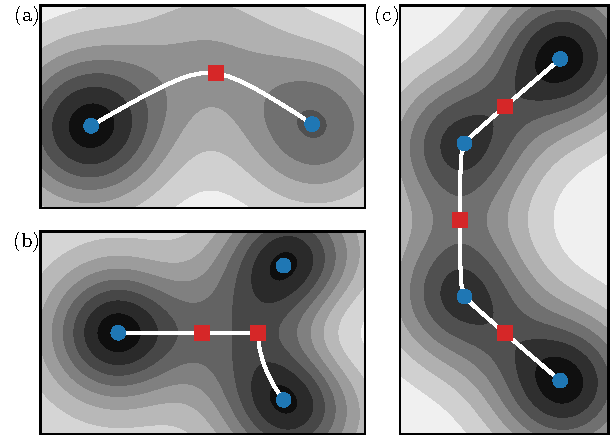
\includegraphics{features.pdf}
  \caption{\label{fig:el-features}
    Schematics showing 2D energy landscapes with the features of interest.
    Blue circles represent the minima, red squares show the transition states, and white paths show the MEPs.
    (a) A simple landscape with two minima connected by a single MEP.
    (b) A landscape where an MEP should terminate at a transition state.
        However, running downhill from the left-most transition state goes past this and continues to a minimum.
    (c) A multi-step pathway with two intermediate minima.
        The full MEP between the top and bottom minima is a combination of the three individual MEPs.
  }
\end{figure}
An energy landscape describes how the energy of a system changes throughout its configuration space.
These are often very high-dimensional landscapes, as the total number of degrees of freedom are typically very large, particularly when modelling continuous macroscale systems.

The primary points of interest are the stable states.
These correspond to local minima in the energy landscape, as any small perturbation would raise the energy and result in a driving force restoring it back to the minimum.
Mathematically, the energy in the vicinity of a minimum at $\bm{x}_0$ can be expressed as,
\begin{equation}
  E(\bm{x}) = E(\bm{x}_0) + \sum_i \frac{a_i}{2} \left. \frac{\partial^2 E}{\partial x_i^2} \right|_{\bm{x}_0} (x_i - x_{0,i})^2,
  \label{eq:el-criticalpoint}
\end{equation}
where $i$ represents each of the principal directions of curvature, and all of the curvatures, $a_i$, are positive.
Using energy minimisation methods to identify these stable states is central to the exploration of energy landscapes.
As an example, \cref{fig:el-features}(a) shows a 2D landscape containing two minima, as well as highlighting other features of interest.

Each minimum also possesses a basin of attraction, which is the surrounding region of points that will converge to the minimum upon following the gradient downhill.
Taking the analogy of a mountainous landscape, these basins correspond to valleys for which the dividing lines are ridges and watersheds.
The energy depth and the extent of a basin can be used to quantify the stability of the state; the former providing the energy required by a interaction to change the state, while the latter provides the required perturbation size.

Transition states (TS) are first-order saddle points on the energy landscape.
These are stationary points where the energy is defined by \cref{eq:el-criticalpoint} with a single negative curvature, $a_1 < 0$, while all others are positive or zero, $a_{i>1} \ge 0$.
These correspond to minima on the ridges separating basins of attraction, so they provide the lowest possible energy required to swap between two stable states.
This energy barrier is incredibly useful for quantifying the stability of states and the probability of a transition between them \cite{Mokkonen2016}.
The energy barrier is also an important quantity to estimate transition times in microscale systems, such as chemical reactions, using transition state theory \cite{Truhlar1996}.
Each transition state also uniquely defines a possible reconfiguration pathway, known as the minimum energy pathway (MEP).

The MEP, $\bm{x}(s)$, connects the transition state to its adjacent minima by following the path of steepest descent from either side of the saddle point,
\begin{equation}
  \deriv{\bm{x}}{s} = \hat{\tau} = - \frac{\grad E(\bm{x})} {|\grad E(\bm{x})|}.
\end{equation}
Here the pathway parameter $s$ is the integrated path length, so the derivative is the unit tangent vector of the pathway.
Therefore, if a transition state has already been found it is a simple process to obtain the MEP.
An equivalent statement, that can provide a convergence criterion for pathway search algorithms, is that the local gradient has no component perpendicular to the direction of the pathway at all points on its length,
\begin{equation}
  \grad^\perp E(\bm{x}) = \grad E(\bm{x}) - (\bm{\hat{\tau}} \cdot \grad E(\bm{x})) \bm{\hat{\tau}} = 0.
  \label{eq:el-mep-convergence}
\end{equation}

Sometimes the precise MEP can end at a transition state rather than a minimum if the steepest-descent pathway reaches a bifurcation point \cite{Wales2004}.
A separate MEP then runs downhill from this to the minima (or to other transition states).
However, in practice, small deviations from the steepest pathway will cause a breaking of symmetry in both experiment and simulations, and it will proceed all the way to one of the minima.
An example of this is shown in \cref{fig:el-features}(b).
MEPs can also be obtained between states that are separated by intermediate minima.
In this case, the MEP will consist of the combination of the individual MEPs between each adjacent pair of minima, each passing over a separate transition state (\cref{fig:el-features}(c)).
Hence, it is possible to build up a network of pathways between adjacent minima to identify all possible reconfiguration pathways of a system.
A single pair of minima can also have multiple pathways between them, even if they are adjacent to one another.
These different pathways can often be difficult to locate and there can be a large number of them in a high-dimensional landscape.
However, the most important are those with the lowest energy and most direct, which are the most easily identifiable.

The MEPs that are located are time independent, providing no direct information about the dynamics along the pathway.
On one hand, this allows energy landscape methods to be more efficient than performing the corresponding dynamical simulations, such as molecular dynamics or finite element analysis, particularly in the case of rare event transitions with barriers larger than $k_\mathrm{B}T$ \cite{Passerone2001}.
On the other hand, the true pathway taken by the system will depend upon the force driving the transition, and inertial effects can cause it to deviate from the steepest descent pathway.
Therefore, the MEP instead provides an ideal pathway that is independent of the force driving the reconfiguration, and provides the average and most probable path that will be taken if driven by random forces or thermal noise \cite{E2007}.

\section{Visualising energy landscapes}
It can be difficult to visualise the high-dimensional landscapes, but one simple way of doing so is using disconnectivity graphs \cite{Wales2004}.
These have a vertical axis showing the energies of all the minima and the transition states with the minimum required energies that connect them.
Such visualisations are useful because they clearly separate the energy landscape into a hierarchy of groups of states according to the ease of reconfiguring between them.
Additionally, the system can be characterised according to the shape of the graph \cite{Wales1998}.
If the energy barriers are tall the system will be trapped it in a single state, and it is referred to as a glassy landscape.
In contrast, small barriers allow the system to easily explore the landscape.
This can be seen by contrasting \cref{fig:el-disconnectivity}(a) and \cref{fig:el-disconnectivity}(b).
Furthermore, the energy landscape may be funnel-shaped, in which case it can quickly converge to the global minimum (\cref{fig:el-disconnectivity}(b)), while for a flat landscape (\cref{fig:el-disconnectivity}(c)) the system is not biased toward any particular state.

\section{Free energy landscapes}
An important concept for characterising the behaviour of a system is that of free energy landscapes.
Until now the discussion has focused mainly upon potential energy landscapes which differ from free energy landscapes in a couple of key ways.
Firstly, while potential energy landscapes are high-dimensional and depend upon all coordinates of the system, free energy landscapes often involve averaging over the coordinates to produce a lower-dimensional system that represents the overall behaviour \cite{Wales2004}.
Also, the free energy includes information about the thermodynamic nature of the system, because separate minima in the potential energy can correspond to a single minimum in the free energy if it can freely swap between them.
Therefore, the free energy landscape changes depending upon the temperature.

\Cref{fig:el-disconnectivity}(d) shows an example of this for a particle cluster, where the potential energy landscape has been reduced to a two-dimensional free energy landscape.
These two order parameters are the potential energy, $V$, and a face-centered cubic packing order parameter, $Q_4$.
Although, in this example there are no free energy minima with high $Q_4$.
At a high temperature there is just a single minimum for high potential energy states, which correspond to a liquid phase.
As the temperature lowers another minimum appears with low potential energy, representing the crystallised structure.
At this point the liquid and crystal states are both stable.
Finally, at the lowest temperatures the liquid minimum disappears and the cluster will only be found in its highly ordered configuration.

This distinction between free and potential energy landscapes are important for microscale and particulate systems where thermal noise is sufficient for the system to spontaneously explore different states.
However, for macroscale systems, which this thesis primarily focusses upon, we are already dealing with effective free energy models that correspond to a thermodynamic average of microstates.
Although there may be some random perturbing effects, such as vibrations, we generally do not consider any further averaging of the states.
Therefore, for brevity, we will simply term our study as an exploration of energy landscapes.

\begin{figure}
  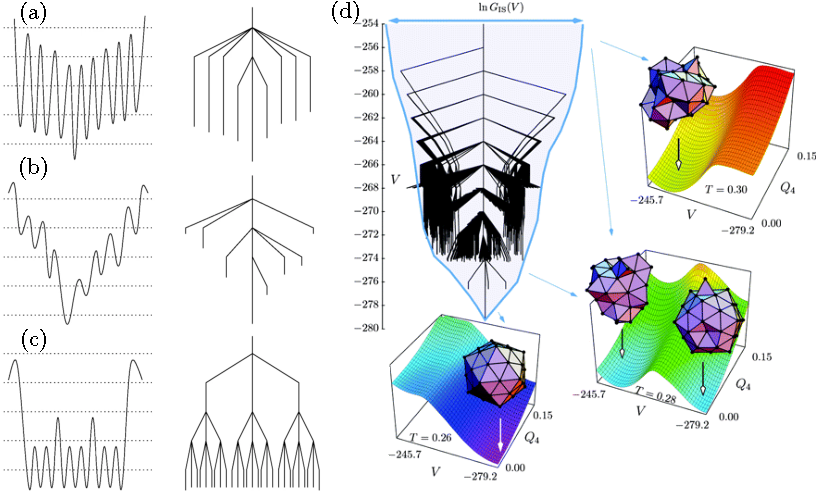
\includegraphics{disconnectivity}
  \caption{\label{fig:el-disconnectivity}
    (a-c) Disconnectivity graphs for three one-dimensional potentials, each exhibiting a different behaviour (see text for discussion).
    (d) Disconnectivity graph for a 55 particle cluster, with the envelope size representing the number of states at, or below, that energy.
        Three 2D free energy landscapes show the states of the system at different temperatures.
        Representative configurations are shown in each of the minima.
        Adapted with permission from \cite{Wales2006}.
  }
\end{figure}



\section{Applications of energy landscapes}
\begin{figure}
  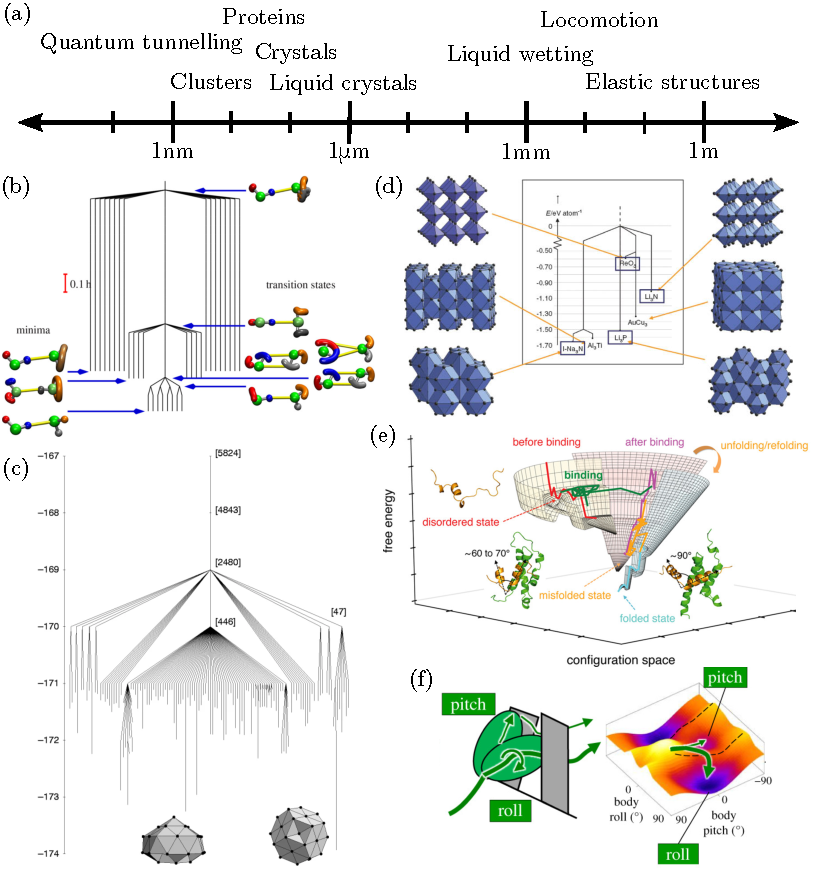
\includegraphics{applications}
  \caption{
    (a) Approximate length scales of various applications of energy landscapes techniques.
    (b) Energy landscape of a pair of hydrogen molecules where the transition states show instanton tunnelling pathways.
        Adapted with permission from \cite{Vaillant2019}.
    (c) Energy landscape showing the candidates for the crystal structure of $\mathrm{Na_3N}$.
        Adapted with permission from \cite{Jansen2014}.
    (d) Disconnectivity graph for a Lennard-Jones 38 particle cluster showing a large funnel for the native icosahedral structure, and a smaller funnel for the truncated octahedron structure.
        Adapted with permission from \cite{Wales1998}.
    (e) Energy landscape of an intrinsically disordered protein, pKID, that folds upon binding with another molecule.
        Adapted with permission from \cite{Chong2019}.
    (f) Diagram showing the two modes of locomotion to pass a barrier and the associate energy landscape.
        This shows the locomotor transition from the pitching to rolling motion.
        Adapted with permission from \cite{Othayoth2021}.
  }
  \label{fig:el-applications}
\end{figure}
Here, we will summarise known applications of energy landscape studies.
To illustrate their wide applicability, we will discuss phenomena across several orders of magnitude, from less than 1\si{nm} to larger than 1\si{m}.

To date, energy landscapes exploration techniques see their most prominent applications in particulate and molecular systems.
At the smallest scales, these are used to study the transition pathways of chemical reactions, where the stable states represent the reactants and products, as well as any reaction intermediates.
Such applications are the source of the term `transition state' which has particular importance for finding reaction rates according to transition state theory.

To obtain accurate chemical reaction rates it is often necessary to consider the effects of quantum tunnelling, which can cause transitions to occur that are classically disallowed.
It is possible to use information about energy barriers and MEP to provide tunnelling corrections to the classical rates from transition state theory \cite{Truhlar1971,Miller1979}.
However, quantum tunnelling depends upon the width of a barrier, not just its height, so shorter paths than the MEP may be more important for determining accurate tunnelling rates.
One approach is to use instantons, which are based upon the path integral formulation of quantum mechanics.
These provide a temperature-dependent pathway that `cuts the corner' of the MEP, providing a more direct path at the expense of a higher barrier \cite{Richardson2016,Richardson2018}.
By finding the transition states of these instantons the effective energy barriers of the transition can be determined, providing more accurate tunnelling rates \cite{Vaillant2019}.

Another topic important to many chemical reactions is that of catalysis, which has been used with energy landscapes for both biological and industrial processes \cite{Boehr2006,Benkovic2008,Kerns2015,Guo2018a}.
This involves a catalyst introducing intermediate reaction steps in order to reduce the maximum energy barrier and increase the reaction rate \cite{Kerns2015}.
These additional reaction steps, as well as multiple possible competing pathways \cite{Benkovic2008}, make it necessary to study the entire energy landscape in order to gain an accurate understanding of the effect that a catalyst will have.

Moving to slightly larger scales beyond chemical reactions, energy landscapes can be used to investigate the formation and rearrangement of complex structures, of which protein folding is perhaps the most pertinent \cite{Bryngelson1995,Onuchic1997}.
Proteins are made up of a very long chain of amino acids and, since the number of stable states tends to grow exponentially with system size, can fold into 3d structures with an incredibly large number of configurations.
In fact, assuming the protein performs a random walk through these structures it may take considerably longer than the age of the universe to find a given state.
And yet, in nature many proteins spontaneously fold to a single state at short timescales.
This is Levinthal's paradox \cite{Zwanzig1992}, and can be resolved using energy landscapes \cite{Bryngelson1995}.
The landscapes of these proteins are found to be highly funnel-shaped and so the protein does not perform a random search, but is instead driven quickly towards the global minimum configuration.
Many proteins can also be found in multiple states, or are intrinsically disordered proteins that do not fold into any particular states \cite{Chong2019}.
Such proteins can be identified by the shape of their landscapes, according to the number of funnels, or if the landscape is flat, respectively.
The misfolding of proteins is also important to study \cite{Yu2015}, owing to the role aggregates of misfolded proteins play in diseases such as Alzheimer's and Parkinson's, or the infectious misfolding that causes prion diseases.
In this case the transition pathways can provide insight into cause of the misfolding, as well as the rate at which it occurs.

Particle clusters, which have widespread applications from catalysis to nanotechnology, are another well studied subject in the context of energy landscapes.
Here the landscapes are often characterised using disconnectivity graphs in order to understand the structural arrangements formed by a given system, as well as properties such as relaxation timescales \cite{Wales1998,Wales2012}
As an example, the Lennard-Jones 38 particle cluster is found to have a double funnel landscape producing either a truncated octahedral or icosahedral structure \cite{Doye1999}.
The truncated octahedron is the global minimum configuration and so might be expected to be favoured.
However, the icosahedral funnel is much wider with more states, explaining why this state is generally favoured.
Related are crystalline solids, which differ due to their lack of a surface, but use energy landscape analysis similarly.
For example, free energy minima have been surveyed to predict the stable structures for a given chemical system \cite{Oganov2009,Jansen2014,Allan2021}, and energy barriers have been used to study phase transitions \cite{Jansen2010}, nucleation \cite{Richard2018}, and defects \cite{Ogata2005,Allan2021}.

In contrast to crystal structures, which tend to have simple funnel landscapes, amorphous solids, glasses, and granular materials all have very complex energy landscapes with high barriers that cause them to get stuck in local minima when cooled below a critical temperature.
Due to the huge complexity in these structures the statistical properties of the energy landscapes are investigated to gain insight into their behaviour \cite{Heuer2008,Raza2015}.
Notably, the glassy landscapes tend to contain fractal basins that result in a secondary relaxation, even if large scale rearrangements are blocked \cite{Charbonneau2014}.
This causes aging of the materials as the structure switches to progressively deeper basins in the landscape \cite{Raza2015}.
Shear strain has been found to affect this aging process by moving into shallower or deeper minima depending on size of strain \cite{Lacks2004,Jin2017}.
Studies have also looked at glassy landscapes for a variety of different topics, such as active matter \cite{Morse2021} and soft glassy materials \cite{Hwang2016}.

Another topic involving the collective arrangement of many particles is liquid crystals \cite{Chakrabarti2008,Kusumaatmaja2015a,Kusumaatmaja2015}.
Here, the transitions between different orientational arrangements are of particular interest for their applications in liquid crystal displays.
Much like the other microscale systems described so far, these can be studied using particulate models \cite{Chakrabarti2008}.
In this case, each particle is given an orientation and anisotropic interactions are used.
On the other hand, because liquid crystal systems involve a large number of particles, continuum phase-field models can be used to represent the smooth variation of the particle orientations \cite{Kusumaatmaja2015a,Kusumaatmaja2015}.
Liquid crystals can therefore be considered somewhere between the microscale, particulate systems, and the macroscale which are often represented by continuum models.

Progressing to larger scale systems, liquid wetting on surfaces has also been studied using energy landscapes \cite{Ren2014,Panter2019a}.
Similarly to the liquid crystals, these often use a continuum phase-field model that uses a smoothly varying order parameter to represent different fluids.
Wetting is important for both biological systems and engineering applications, and one topic relevant to both is structured surfaces.
These can introduce superhydrophobicity by suspending droplets so they can be easily shed, keeping the surface dry.
Using energy landscapes these structures have been investigated to identify how this suspended droplet state may fail, and how this can be avoided \cite{Ren2014,Panter2019a}.

Even highly non-equilibrium systems can benefit from the use of energy landscapes, for example, transition pathways have been used to describe locomotor transitions in animals \cite{Othayoth2020,Othayoth2021}.
This represents different modes of motion (climbing, walking, rolling, etc.) as minima in a free-energy landscape.
This landscape is modified by interaction with the environment, which changes the energy barriers associated with locomotor transitions, and can cause them to occur spontaneously.
This is seen, for example, in the motion of a cockroach either climbing or rolling past grass-like barriers \cite{Othayoth2020}.

Among some of these largest scale applications using energy landscapes (but by no means the upper limit) are elastic structures.
Here the primary interest lies in the structural changes between different states, so pathway analysis will be important.
In the following chapter, the different types of elastic structures will be discussed as well as the existing work that has been performed using the theory of energy landscapes.

  \chapter{Elastic Structures}
\label{ch:elastic_structures}
\graphicspath{{elastic_structures/fig/}}

Elastic behaviour is ubiquitous in both nature and engineering applications, and in many cases, they exhibit multistability and can reversibly change between different configurations.
Such systems have wide-ranging potential applications, such as deployable structures \cite{Filipov2015,Zhai2018,Zareei2020}, micro-electromechanical systems \cite{Felton2014,Ko2017}, robotics \cite{Kwok2014,Chen2018a,Gorissen2020,Currier2020,Tang2020}, and energy absorption \cite{Shan2015,Bertoldi2017a}.
These are often complex structures, but the multistable behaviour is usually derived from simple elements, such as buckled beams or surfaces, and elastic joints or creases.
In this chapter various types of multistable elastic structures will be outlined, along with some of the recent and ongoing research on this topic.



\section{Buckling}
Buckling is a sudden change of shape that occurs when a structure is subject to compressive strain.
Generally, this is an undesired effect that is associated with structural failure and can have severe consequences, particularly if it occurs in buildings or other infrastructure.
Therefore, fields such as structural engineering utilise a range of techniques to prevent buckling and ensure the stability of structures.
However, recently there has been significant interest in exploiting buckling transitions to develop flexible devices and structures that can reversibly transform from an undeformed state to a buckled state, or between two different buckled states.
Some key examples will be discussed here.

The most basic, and perhaps most versatile, buckled system is that of a column or thin beam under compression.
This is possible to be monostable or bistable, depending upon the strain applied and angles at which the end points are held.
Previous research has extensively surveyed the stability of the states under different sets of parameters \cite{Wan2020}.
This can therefore be applied to understand the behaviour of more complex structures constructed from simple beam elements.

\begin{figure}[htb]
  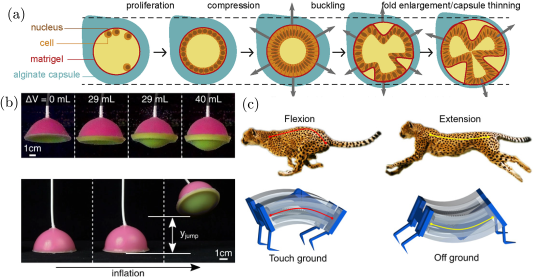
\includegraphics[width=\textwidth]{buckling.png}
  \caption{
    (a) Schematic showing how the growth of a membrane of cells can lead to buckling and the formation of folds.
        Adapted with permission from \cite{Trushko2020}.
    (b) A soft jumper that uses the snap-through buckling of a spherical shell upon inflation.
        Adapted with permission from \cite{Gorissen2020}.
    (c) A cheetah-inspired soft actuator for robotic movement.
        A central bistable linkage is used in combination with with inflatable channels to change states.
        Adapted with permission from \cite{Tang2020}.
  }
  \label{fig:es-buckling}
\end{figure}

While global buckling modes are typically observed in thin beams, surfaces and thin shells can exhibit local buckle through the formation of dimples on the surface.
This is generally undesired in engineering applications, such as containers or rockets, and is important to understand how it occurs in order to prevent and control structural failure.
The size of disturbances that are required in order to buckle both cylindrical and spherical shells under strain have been investigated by applying probing forces \cite{Virot2017,Hutchinson2018}.
In addition, various works have investigated the effect of imperfections, which can significantly reduce resistance to buckling \cite{Deml1997,Hutchinson2018}.
These findings highlight the precise manufacturing that is required to ensure that buckling cannot occur.

The buckling of surfaces and membranes also plays an important role in various biological functions.
One case is in the formation of folded structures of cell layers, which are essential in many anatomical structures such as glands or crypts.
Buckling is a possible mechanism for the formation of these structures.
For example, it can be caused by the growth of cells when constrained by a surface \cite{Nelson2011,Trushko2020}, \cref{fig:es-buckling}(a).
Many of these biological membranes, such as lipid bilayers, are a liquid surface that can redistribute to reduce local stress, but these too can buckle.
An example of this is the budding of cell membranes, where the binding of curved structures to the membrane can result in stress that causes the surface to buckle \cite{Lenz2009}.
Furthermore, it is possible to use the onset of buckling to measure the mechanical properties of cells \cite{Evans1983}.

% [[In small scale systems, such as in cells, capillary forces of liquids can become significant and deform elastic structures.]]
% [[This is known as elasto-capillarity and involves a competition between surface tension deforming the structure, and the elastic force restoring it.]]
% [[When the surface tension wins out it can cause buckling to occur \cite{Andreotti2011}.]]
% [[Elasto-capillarity can cause cell membranes to deform and engulf droplets \cite{Kusumaatmaja2011}, which is another cause of cell budding.]]
% [[This has also been applied to droplets on substrates with different shapes, which then fold and engulf the droplets into different shapes \cite{Roman2010}.]]
% [[Elasto-capillarity can also lead to the collapse of surfaces and tubes \cite{Roman2010,Emery2021}, as well as the buckling and coilling of elastic rods constrained within a droplet \cite{Elettro2017}.]]

An area where buckling can be highly beneficial is in the development of soft actuators for robotics.
In contrast to traditional robotic motion, soft actuators can provide simpler systems that are lighter, less prone to failure, and safer around humans.
Using buckling instabilities it is possible to amplify actuation of these soft structures, causing large, sudden displacements which can be used for propulsion.
For example, bistable beams have been used to propel swimming robots \cite{Chen2018a}, and the snap-through of spherical shells has been used for inflatable jumpers \cite{Gorissen2020}, shown in \cref{fig:es-buckling}(b).
Buckling can further be used to emulate biological behaviour such as swimming fish \cite{Currier2020}, and the galloping of cheetahs \cite{Tang2020}, \cref{fig:es-buckling}(c).
Finally, bistable structures have been used in pneumatic soft grippers that can be pressurised to pick up objects and continue to hold them even when the pressure is released \cite{Yang2015,Faber2020}.



\section{Buckled mesostructures}\label{sec:es-mesostructures}
The class of elastic structures that will primarily be investigated in this thesis are known as 3D buckled mesostructures.
These are produced as a flat pattern which buckles under a compressive strain to form a three-dimensional structure.
Typically, this is carried out by binding the structure at various points to a pre-stretched substrate, which is then released, compressing the structure.
This provides a simple method for fabricating complex structures, and can be used to create structures down to the microscale.
These have been investigated for applications such as flexible electronics \cite{Fu2018}, microelectromechanical systems \cite{Fu2018,Ning2018}, biomedical devices \cite{McCracken2017,Yan2017}, and microrobotics \cite{Yan2017}.

Many works have investigated the resultant three-dimensional structures for various different precursor patterns.
Simple patterns may consist of a single ribbon or a connected grid of ribbons with periodic bonding sites, in which case the ribbons will buckle into a wavy structure, \cref{fig:es-mesostructures}(a).
Or if the ribbons are curved, they can twist into helical coil shape when buckled \cite{Xu2015}.
By connecting these ribbons together in complex networks, it is possible to create multilevel, buckled designs.
Generally, these structures will buckle up fully.
However, if the adhesive force to the substrate is strong ,such as for very small scale structures, it may remain attached to the substrate in various locations \cite{Liu2019}.

\begin{figure}[htb]
  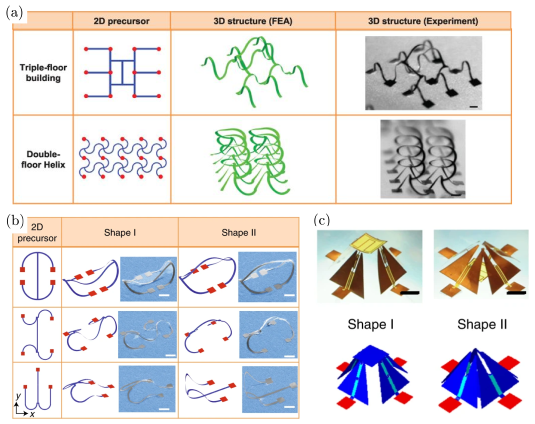
\includegraphics{mesostructures.png}
  \label{fig:es-mesostructures}
  \caption{
    (a) Buckled mesostructures with patterns that produce multilevel structures.
        Adapted with permission from \cite{Xu2015}.
    (b) Multistable mesostructures that can each take two different buckled states.
        Adapted with permission from \cite{Fu2018}.
    (c) A multistable mesostructure with a radio-frequency antenna on top.
        In shape 1 the antenna is free to transmit, but in state 2 it is blocked.
        Adapted with permission from \cite{Silverberg2014}.
  }
\end{figure}

It is possible for some mesostructures to buckle into multiple different stable configurations, such as those seen in \cref{fig:es-mesostructures}(b).
However, these structures are limited and it may be difficult to obtain more than a single state in practice.
This multistability can be enhanced by incorporating origami-like creases into the structure where it can more easily bend \cite{Fu2018}.
This greatly increases the variety of structures with multiple stable stables and allows greater control over which states are stable.
This can be utilised to create switchable devices, such as an antenna that can transmit in one configuration, but is shielded in another, as depicted in \cref{fig:es-mesostructures}(c).

A number of different approaches have been suggested in order to obtain these different states.
Fu et al. \cite{Fu2018} discovered a method of producing different shapes by controlling the release of the underlying substrate over time.
By independently releasing the substrate in different directions they were able to obtain structures with three separate states.
In this approach, the available states are limited to those that are spontaneous under buckling.
Park et al. \cite{Park2019} were able to control the shape of the structure over time by dissolving a constricting film.
However, this approach is irreversible and the possible shapes are limited.
Furthermore, they suggested a method for keeping the mesostructures buckled after removing from the substrate, by interlocking parts of the structure to keep it in place.
A different approach has been considered by Hao et al. \cite{Hao2020}.
Instead of using a stretched substrate, they used structures made from hydrogels which swell, causing the structure to buckle.
They were able to control the buckling to obtain various stable configurations by preswelling parts of the structure.

Despite these methods for creating multiple stable states, reconfigurability after the structure is created has largely remained unaddressed.
An approach addressing this problem will motivate later work in \cref{ch:mesostructures,ch:origami_ribbon}.



\section{Mechanical metamaterials}\label{sec:es-metamaterials}
Although we focus primarily upon buckled mesostructures in this thesis, it is worth considering the related, and popular topic of mechanical metamaterials.
These are materials that have properties defined by their structure and not the properties of the constituent material.
They can show a variety of interesting and unusual properties such as negative Poisson ratio (auxetic materials) \cite{Bertoldi2017,Bertoldi2017a}, where the material expands (or contracts) in all directions simultaneously, or negative compressiblity \cite{Nicolaou2012,Lakes2001}, where the material contracts under a tensile force.
There are many different types of mechanical metamaterials, but each of which is typically made up of a repeating pattern of simple elements, such as beams or hinges \cite{Bertoldi2017}.
If these individual elements are multistable by undergoing a buckling transition, then the metamaterial itself will be multistable.

Some metamaterials can have large numbers of elements that buckle at once under compression or tension \cite{Che2017,Bertoldi2017a}.
An example is the 3D elastomeric structure shown in \cref{fig:es-metamaterials}(a), where the array of holes can collectively buckle, resulting in a highly non-linear compressive behaviour with a negative Poisson ratio \cite{Bertoldi2010,Florijn2014,Bertoldi2017a,Medina2020}.
Similar structures with buckling beams have also been proposed for energy absorption and storage \cite{Shan2015,Che2017,Bertoldi2017a,Giri2021}.
These have advantages over traditional materials used for collision protection because they can easily unbuckled and reused.
The structures can also exhibit hysteresis loops under cyclic loading and unloading, and so can be used for dissipating energy and damping vibration \cite{Bertoldi2017a}.
The order of buckling in these structures is unpredictable because each cell is identical and will depend upon manufacturing imperfections, but this can be controlled by varying the thickness of the bistable beams \cite{Che2017,Giri2021}.

Energy absorbing metamaterials are generally constructed in arrays, with rows of cells that buckle together, but not all at once.
However, for some metamaterials, the transition of one cell can destabilise neighbouring sections and lead to a cascade across the entire structure.
These are attractive for realising complex, self-deploying structures \cite{Zareei2020}.
The change of state occurs through transition waves that travel at a constant speed through the structure, behaving similarly to phase transitions observed in crystalline solids \cite{Jin2020}.
The transition waves can also be controlled and redirected by introducing defects into the periodic structure, as seen in \cref{fig:es-metamaterials}(b).

% Opposite to this are mechanical metamaterials are able to support local multistability by the buckling of individual elements.
% These structures can be programmed to set material properties such as stiffness \cite{Silverberg2014,Florijn2014,Chen2021}.
% For example, a metamaterial containing holes, similar to that in \cref{fig:es-metamaterials}(a), can be laterally confined at chosen locations.
% As this number of confined locations is increased, the mechanical response becomes more and more non-monotonic and hysteretic \cite{Florijn2014}.
% Another metamaterial has been demonstrated that is constructed of elements that contain a stopper that buckles up or down to block or allow compression \cite{Chen2021}.
% These can be individually switched between the two states on-demand, using a magnetic force.
% Two- or Three-dimensional arrays can therefore be constructed to produce a metamaterial with a reprogrammable and fine-tunable stiffness.

In addition to exhibiting interesting behaviour under compression, metamaterials can also be used to create multifunctional structures that morph into a variety of different configurations \cite{Shim2012,Haghpanah2016,Overvelde2017,Iniguez-Rabago2019,Zareei2020}.
One approach consists of tessellating prismatic structures with flexible hinges, \cref{fig:es-metamaterials}(c), which are able to change into a large variety of different shapes thanks to their 3D structure \cite{Overvelde2017,Iniguez-Rabago2019}.
These can be used to create structures that modify their shape and behaviour based upon changing environments, and be used to perform multiple tasks.
These structures are able to remain in the different configurations without an applied force because of multiple stable states resulting from the buckling of the rigid faces \cite{Iniguez-Rabago2019}.
A similar idea is seen in \cite{Shim2012}.
Here, the authors design a metamaterial that consists of an elastic spherical sphere that can undergo transformation from a large sphere with a relatively open surface to a small sphere with a dense surface.
Such a device could offer reversible encapsulation functionality in order to transport small quantities of substances.

\begin{figure}[htb]
  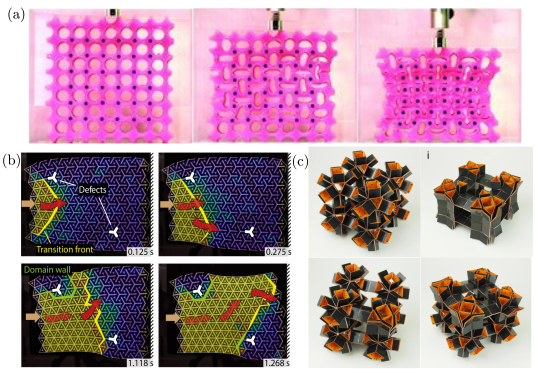
\includegraphics{metamaterials.png}
  \label{fig:es-metamaterials}
  \caption{
    (a) An elastic metamaterial with holes that buckle under compression.
        Adapted with permission from \cite{Overvelde2012}.
    (b) A transition wave through an auxetic metamaterial that is redirected by lattice defects.
        Adapted with permission from \cite{Jin2020}.
    (c) A 3D prismatic metamaterial that is able to reconfigure into a variety of stable states.
        Adapted with permission from \cite{Iniguez-Rabago2019}.
  }
\end{figure}



\section{Origami}
Origami structures are a specific type of mechanical metamaterial that have garnered considerable attention in particular.
They consist of a network of rigid flat surfaces joined by creases that are free to bend, which enables simple two-dimensional surfaces to form complex three-dimensional structures.
Origami is used for both artistic purposes and engineering applications, largely for its ability to produce strong, but light structures and materials \cite{Lv2014}.
One particularly useful class of origami structures are those that can fold from a flat surface, known as flat foldable, and are therefore easy to produce.
The simple reconfigurability of flat foldable structures also makes them suitable for deployable structures, such as solar panels for satellites \cite{Miura1985,Evans2015}.

By considering elastic folds with an optimal angle and allowing some bending of the rigid faces, many origami structures are found to be multistable.
Indeed, one of the most basic components of origami (vertices of four creases) is multistable \cite{Waitukaitis2015} and that these can be tiled to create large reconfigurable structures.
One such tiled structure is the Miura-ori pattern, \cref{fig:es-origami}(b), which is well known for its ability to unfold from a compact structure to a flat surface in a single motion as a result of a negative Poisson ratio \cite{Miura1985,Evans2015}.
For this usage, the structure is elastically monostable and therefore requires actuation to remain in a deployed state.
Bistability has been observed, however, through the inversion of singular cells of the Miura-ori pattern to create ``pop-through defects''.
These can be introduced to programmatically modify the stiffness of the structure, while remaining completely reversible \cite{Silverberg2014}.

Beyond simple sheets, origami can be used to produce three-dimensional structures.
For example, by stacking origami sheets, cellular metamaterials can be produced that are auxetic or can be used for impact energy absorption \cite{Fang2017,Harris2021}.
The behaviour is then easily tunable by modifying the underlying two-dimensional fold pattern.
Alternatively, the origami sheets can be curved and turned into tubes and cylinders \cite{Filipov2015,Zhai2018}.
These tubes are then able to easily extend and collapse simply by deforming the end, providing another useful approach for realising deployable structures.

Kirigami is a variation of origami whereby cuts are introduced into the surface in addition to folding.
This allows for structures with greater flexibility and additional stable states, with each end of a cut able to take one of two different states \cite{Sadik2021}.
The introduction of cuts also allows the structure to deform and buckle under compression \cite{Brighenti2005}, which has been exploited to create a variety of simple actuators that rotate or lift \cite{Dias2017}.

\begin{figure}
  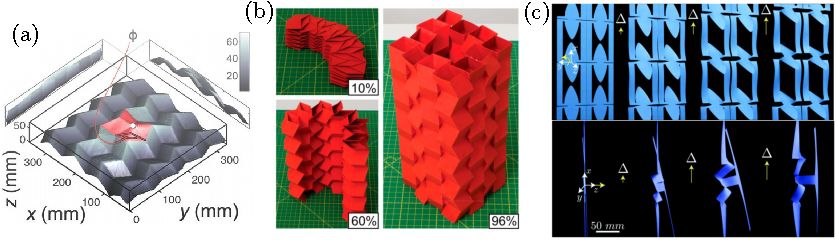
\includegraphics[width=\textwidth]{origami.pdf}
  \caption{
    (a) A Miura-ori pattern with a pop-through defect (red) that alters the stiffness of the structure. 
        Adapted with permission from \cite{Silverberg2014}.
    (b) A combination of 12 origami tubes that deploy to produce an enclosed structure.
        Adapted with permission from \cite{Filipov2015}.
    (c) Two kirigami actuators that rotate and lift, respectively, when extended.
        Adapted with permission from \cite{Dias2017}.
  }
  \label{fig:es-origami}
\end{figure}



\section{Energy landscapes applied to elastic structures}
Recently there has been increasing interest in using energy landscape methods to investigate multistable elastic structures \cite{Iniguez-Rabago2019,Medina2020,Silverberg2015,Zhai2018,Hutchinson2018,Virot2017,Panter2019}.
Since these structures are primarily macroscopic, thermal effects are insignificant and are external forces are needed to reconfigure them instead.
Correspondingly, there is no need to investigate their statistical behaviour.
Instead, energy landscape analysis can be used to design structures, and to inform how best to reconfigure them.
% The latter being particularly important owing to the complex and highly non-linear pathways that these structures often have.

Perhaps the most common use of energy landscapes in the field is to determine the various states that a given structure can take for given structural parameters.
For example, this has been used in the study of some reconfigurable mechanical metamaterials.
Iniguez-Rabago et al. have looked into several shape-changing 3D prismatic structures \cite{Iniguez-Rabago2019}.
By varying just two of the fold angles they were able to produce a simplified landscape, shown in \cref{fig:es-landscapes}(a), displaying the stable regions of each of the structure's various states.
A similar survey was also carried out for the elastomeric metamaterial with cylindrical holes that buckles under compression \cite{Medina2020}.
To understand how it behaves when compressed, all of the possible states were identified at increasing levels of strain, \cref{fig:es-landscapes}(b).
Furthermore, by introducing slight imperfections to the structure they were able to identify which of the states are obtained upon experimentally deforming the system.

% The central building block for many multistable elastic structures are compressed beams, which are bistable.
% Energy landscape surveys have been performed for these to determine for what strain and angles the beam will take different states \cite{Wan2020}.
% The landscapes of such a beam are simple, yet important, owing to their many uses, for example in metamaterials that absorb energy under compression \cite{Shan2015}.
% For this, the buckling pathways have been studied to find the energy barrier and force curves.
% The barriers have also been modified by changing the thickness of the beams in the structure in order to control the order that they buckle \cite{Che2017,Giri2021}.

% Another multistable structure is the square twist, an auxetic structure made up of square and rhombus faces.
% This undergoes a bistable transition from an unfolded state to a folded state, during which the faces are required to bend.
% This structure has been studied in detail in \cite{Silverberg2015} where a minimum angle is identified for the rhombus faces that gives a bistable structure, and as the stiffness of the faces is increased, this critical angle reduces to zero.

Energy landscapes have also been utilised in the study of origami structures.
In particular, these have looked at the reconfiguration pathways, which are often complex and non-linear due to the folding through large angles.
% Some studies have sought to locate these to describe the functionality of the origami structures and the ease with which they can be refolded.
Silverberg et al. \cite{Silverberg2015} investigated the square twist structure which undergoes a bistable transition from an unfolded to folded state, during which the faces are required to bend.
They were able to identify how the rigidity and shape of the structure affected the transition pathway and its barrier, and thereby how they could be tuned for specific applications.
Another use of the pathway is demonstrated for an origami cylinder \cite{Zhai2018}, which is easily deployable as a result of the small energy barrier.
In this case, the MEP causes the cylinder to first extend beyond its deployed state before returning.
Therefore, the structure must take a different pathway when the deployed structure is placed under compression, ultimately resulting in a much higher energy barrier and stiffness.
However, in each of these cases the pathways have been identified by applying forces to the structure, rather than locating the MEP.

Recently, MEP methods have also enabled the identification of completely rigid folding pathways in origami structures, even when crease bending energy is disregarded, such that there is no energy barrier between the unfolded and folded states.
By employing a pathway search algorithm that was fixed at the two end points with an energy that penalised any deviations from rigid folding, Zhou et al. were able to locate the rigid folding pathway for the Miura-ori pattern \cite{Zhou2023}.
A similar method could also be applied to other reconfigurable structures that are not necessarily multistable, as long as the two end states to be known.
% In the same study a bistable structure, the waterbomb base, is also considered, as well as a joined array of these structures.
% This time crease bending is considered in order to identify the energy barriers between the stable states, which turn out to be several orders of magnitude higher than the initial estimate.

In addition to providing information about desired reconfigurabilty, pathway analysis can be used to identify the failure modes of a system.
For example, the buckling of spherical and cylindrical shells under axial compression is hard to predict and depends strongly upon the size of any imperfections \cite{Hutchinson2018}.
However, by studying the energy barrier it is possible to identify how these imperfections affect the critical pressure before buckling occurs \cite{Hutchinson2018,Virot2017}.
Further work has also been undertaken to identify how the shape of the cylinders affects the structure of the energy landscape \cite{Panter2019}.
Panter et al. identified that short cylinders had simple funnelled landscapes, and long cylinders had complex landscapes with many more minima.
Furthermore, using the information about the initial buckling transition state, they were able to modify the distribution of the structure's thickness in order to maximise the energy barrier, and to control the energy landscape, reducing the number of states, \cref{fig:es-landscapes}(d).

\begin{figure}[htb]
  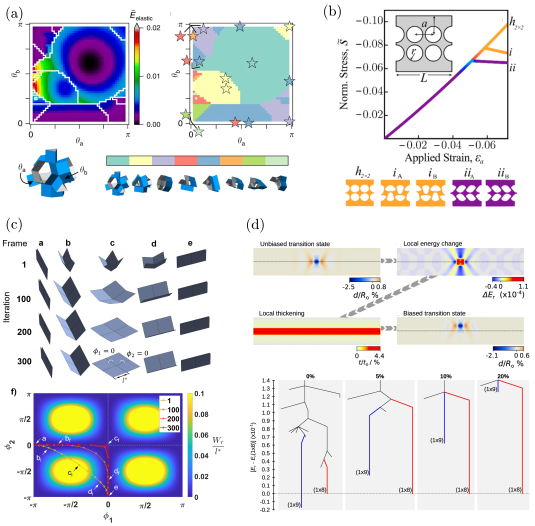
\includegraphics{landscapes.png}
  \label{fig:es-landscapes}
  \caption{
    Energy landscape methods applied to various elastic structures.
    (a) The landscape of a prismatic structure when varying two of the angles.
        The elastic energies of each configuration are shown on the left, and the basins of attraction for each state are on the right.
        Adapted with permission from \cite{Iniguez-Rabago2019}.
    (b) The stable states of a $2\times2$ holar metamaterial at different values of the compressive strain.
        Adapted with permission from \cite{Medina2020}.
    (c) Identifying the rigid folding pathway of a Miura-ori vertex using an NEB pathway.
        The top shows snapshots along the pathway as it is optimised.
        At the bottom the 2D energy landscape is shown.
        The pathway is refined towards the rigid folding pathway where the energy is zero.
        Adapted with permission from \cite{Zhou2023}.
    (d) Using information about the transition state of the buckling of a cylinder to alter the buckling behaviour.
        The top shows how the thickness is increased where the bending energy of the transition state is locally higher, resulting in an altered transition state.
        The bottom shows that, as the thickness is increased, the landscape changes and a low energy state is suppressed.
        Adapted with permission from \cite{Panter2019}.
  }
\end{figure}

  \chapter{Energy Landscape Methods}
\label{ch:methods}
\graphicspath{{methods/fig/}}

In this chapter we will explore some of the existing methods for energy landscape exploration.
Then we will discuss the advantages and disadvantages for each of the methods, including their use for elastic structures and other continuous systems.
It is not feasible to discuss all such methods, so we will restrict our focus to some of the most commonly used approaches.

Firstly, we will look at energy minimisation methods, which are central to the exploration of energy landscapes.
They are used to locate local minima in the landscapes, and are utilised in almost all energy landscape methods to find saddle points and minimum energy pathways.
So, efficient minimisation algorithms are crucial.

After this we will look at methods for locating transition states (TS).
These can use a single state to find a nearby TS, so-called single-ended methods, or can use two states that converge towards a TS from either side, known as double-ended methods.
Finally, we will look at some methods for locating minimum energy pathways using a chain of states.
These methods are also often referred to as double-ended transition state methods, while the bracketting methods are often overlooked.
However, here we will not be refer to them as such, and disambiguate between the two groups according to whether a method is primarily locating the pathway or the TS.



\section{Energy minimisation}

\subsection{Gradient descent}
Perhaps the simplest minimisation algorithm is gradient descent.
In this method a point on the landscape is iteratively refined by taking steps in the direction opposite to the gradient.
This causes the point to follow the path of steepest descent towards the local minimum.
Explicitly, the coordinates $\bm{x}_i$ at iteration $i$ are updated according to,
\begin{equation}
  \bm{x}_{i+1} = \bm{x}_i - \alpha_i \grad E(\bm{x_i}).
  \label{eq:lm-graddescent}
\end{equation}
The step size, $\alpha_i$, may be set to a single value, however this would slow down convergence, and may cause the method to diverge if it is too large.
A more common method is to use a line search (described below) to perform a one-dimensional optimisation in the direction of the step.

\subsubsection{Line search}
Given a search direction $\bm{p}$ (for gradient descent $\bm{p} =-\grad E(\bm{x})$) the aim of the line search is to find the step size, $\alpha$, that minimises the function $E(\bm{x}+\alpha\bm{p})$.
An exact solution could be found, but this is likely inefficient.
Instead, it is best to find a value that is good enough and then proceed with the next iteration of the method.
Two common ways of determining this are using the Wolfe conditions \cite{Wolfe1969,Wolfe1971} or a backtracking line search \cite{Armijo1966}.

The Wolfe conditions are that the objective function must reduce sufficiently (the Armijo rule), and that the gradient must also reduce sufficiently (the curvature rule):
\begin{gather}
  E(\bm{x}+\alpha\bm{p}) \le E(\bm{x}) + c_1 \alpha \bm{p} \cdot \grad E(\bm{x}),     \qquad \text{(Armijo rule)}
  \label{eq:lm-ls-armijo}
  \\
  - \bm{p} \cdot \grad E(\bm{x}+\alpha\bm{p}) \le - c_2 \bm{p} \cdot \grad E(\bm{x}). \qquad \text{(Curvature rule)}
  \label{eq:lm-ls-curvature}
\end{gather}
The parameters $c_1$ and $c_2$ must be chosen to satisfy $0 < c_1 < c_2 < 1$.
Each of these rules places a bound on the step size, with the Armijo rule placing a maximum bound, and the curvature rule enacting a minimum bound.

The backtracking line search is a little different.
The Armijo rule is still used to ensure that the step size is not too large, however the curvature rule is not.
Instead, the method first begins with a large step size and incrementally reduces it until it satisfies the Armijo rule.


\subsection{Newton's method}
Newton's method is a second order minimisation method that uses the Hessian to provide a faster rate of convergence than first order methods such as gradient descent.
Each iteration of this method effectively uses the gradient and curvature to fit a paraboloid to the energy landscape surface, and then proceed to the critical point.
As a result, this method may also find maxima or saddle points instead of local minima.

To obtain the step, $\bm{s}_i$, to take from a position $\bm{x}_i$ at iteration $i$, we consider the second-order Taylor expansion,
\begin{equation}
  E(\bm{x}_i + \bm{s}_i) = E(\bm{x}_i) +  \bm{s}_i^\mathrm{T} \grad E(\bm{x}_i) + \frac{1}{2} \bm{s}_i^\mathrm{T} \mathrm{H}(\bm{x}_i) \bm{s}_i,
\end{equation}
where $\mathrm{H}$ is Hessian matrix.
The step should take it to the critical point, where the gradient is zero,
\begin{equation}
  \grad E(\bm{x}_i + \bm{s}_i) = \grad E(\bm{x}_i) + \mathrm{H}(\bm{x}_i) \bm{s}_i = 0.
\end{equation}
So the step that should be taken at each iteration is
\begin{equation}
  \bm{s}_i = - \mathrm{H}^{-1}(\bm{x}_i) \  \grad E(\bm{x}_i).
  \label{eq:lm-newtonstep}
\end{equation}
Once the step has been found it is also possible to perform a line search along that direction.
This can be used to ensure that the energy always reduces and a minimum is found rather than a saddle point or maximum.


\subsection{L-BFGS}
The limited-memory Broyden-Fletcher-Goldfarb-Shanno (L-BFGS) algorithm \cite{Nocedal1980,Liu1989} addresses two difficulties associated with Newton's method.
The first is the calculation of the Hessian, which may be complicated or not known for many systems.
Furthermore, for an $n$-dimensional system it has a computational complexity of $O(n^2)$, so it can be computationally costly for many energy landscapes which have a very large number of dimensions.
The second is the inversion of the Hessian in \cref{eq:lm-newtonstep}, which is even more costly, scaling as $O(n^3)$.
Since L-BFGS is a quasi-Newtonian method which approximates \cref{eq:lm-newtonstep} rather than calculating the Hessian directly, it does not suffer from these same problems.

It is based upon the BFGS algorithm \cite{Fletcher1987}, which continually updates an approximation of the inverse Hessian matrix using the changes to the position and gradient at each iteration.
This prevents the need to know the Hessian, or perform the matrix inversion.
However, the whole matrix $\mathrm{H}^{-1}$ must still be calculated, with a complexity of $O(n^2)$.

L-BFGS addresses this by only storing several vectors representing changes in the positions and gradients of the past $m$ steps ($\bm{s}_j$ and $\bm{y}_j$ for $j=i-m,\ldots,i-1$, respectively), and the approximation of \cref{eq:lm-newtonstep} is calculated directly.
This bypasses the need to calculate the full inverse Hessian matrix, and results in a much lower complexity of $O(nm)$.
To do this, two sets of vectors ($q_j$ and $z_j$ for $j=i-m,\ldots,i$) are calculated iteratively based upon the recursive method used by BFGS.
The first vectors are given by
\begin{align}
  \bm{q}_i &= \grad E(\bm{x}_i),
  \label{eq:lm-lbfgs-q0}
  \\
  \bm{q}_j &= \bm{q}_{j+1} - \left( \frac{\bm{s}_j \cdot \bm{q}_{j+1}} {\bm{s}_j \cdot \bm{y}_j} \right) \bm{y}_j
    \quad \text{for} \quad j = i-1, \ldots, i-m.
  \label{eq:lm-lbfgs-q}
\end{align}
Then the second set of vectors are calculated as
\begin{align}
  \bm{z}_{i-m} &= - \left( \frac{\bm{s}_{i-1} \cdot \bm{y}_{i-1}} {\bm{y}_{i-1}^2} \right) \bm{q}_{i-m},
  \label{eq:lm-lbfgs-z0}
  \\
  \bm{z}_{j+1} &= \bm{z}_j - \left( \frac{\bm{s}_j \cdot \bm{q}_{j+1}} {\bm{s}_j \cdot \bm{y}_j} -
    \frac{\bm{z}_j \cdot \bm{y}_j} {\bm{s}_j \cdot \bm{y}_j} \right) \bm{s}_j
    \quad \text{for} \quad j = i-m, \ldots, i-1.
  \label{eq:lm-lbfgs-z}
\end{align}
The step to take is then given by $\bm{s}_i = \bm{z}_i$.
It is also generally desirable to carry out a line search in this direction to ensure that the step is acceptable and is going downhill.
This is then repeated until convergence is reached.


\subsection{FIRE}
Another useful method is the fast inertial relaxation engine (FIRE) \cite{Bitzek2006}.
Unlike the other methods this uses an inertial minimiser inspired by molecular dynamics.
This involves a velocity, $\bm{v}$, that quantifies the rate of change of the system coordinates, which is driven by the force $\bm{F} = - \grad E(\bm{x})$.
Additional modifications are also made to the velocity in order to drive it more quickly in the downhill direction, or stop if it is moving uphill,
\begin{equation}
  \bm{v} \rightarrow
  \begin{cases}
    \bm{v} + \alpha |\bm{v}| (\bm{\hat{F}} - \bm{\hat{v}}) & \text{if } \bm{v} \cdot \bm{F} > 0\\
    0 & \text{if } \bm{v} \cdot \bm{F} \le 0
  \end{cases}
  \label{eq:FireVelUpdate}
\end{equation}
where $\alpha$ parametrises the downhill velocity modification and $\Delta t$ is the timestep.
These values are also dynamically changed to accelerate the minimisation if it is successfully proceeding downhill:
If $\bm{v} \cdot \bm{F} > 0$ for the past five or more iterations, $\Delta t$ is increased by a factor of 1.1 until it reaches a defined maximum value, and $\alpha$ is reduced by a factor of 0.99.
Otherwise, if $\bm{v} \cdot \bm{F} \le 0$, $\alpha$ is reset to its starting value of 0.1, and the timestep is halved.
In summary the method follows the following algorithm:
\begin{enumerate}[leftmargin=*]
  \item Initialise coordinates $\bm{x}$, and velocity $\bm{v}=\bm{0}$.
  \item Calculate the force $\bm{F} = - \grad E(\bm{x})$.
  \item Update the velocity, $\bm{v} \rightarrow \bm{v} + \bm{F} \Delta t / m$.
  \item Modify the velocity according to \cref{eq:FireVelUpdate}.
  \item Update $\alpha$ and $\Delta t$ depending upon the value of $\bm{v} \cdot \bm{F}$.
  \item Update the position, $\bm{x} \rightarrow \bm{x} + \bm{v} \Delta t$.
  \item Check for convergence, otherwise return to 2.
\end{enumerate}


\subsection{Simulated Annealing}
For some applications, when the gradient is undefined or difficult to calculate it may be necessary to use a gradient-free minimisation algorithm.
This is most typically the case for discrete problems.
Simulated annealing \cite{Kirkpatrick1983} is one such algorithm that is based upon the thermodynamic annealing of metals.
This uses random displacements and chooses whether to accept them depending upon the change in energy.
Unlike the methods above, simulated annealing is primarily a global minimiser because it can jump into the basins of other minima and so is not simply restricted to finding the local minimum closest to its initial position.

For each iteration the random perturbation is chosen such that the new state is not too far from the previous.
This may be performed by adding small perturbations to each degree of freedom separately, or ensuring that the total displacement is below a certain value.
The probability of accepting this depends upon the energies of the proposed state, $E'$, and the current state, $E$, according to a Metropolis acceptance criteria \cite{Metropolis1953},
\begin{equation}
  P(E', E, T) =
  \begin{cases}
    1, & \text{if } E' \le E\\
    \exp( -(E'-E) / T ), & \text{if } E' > E
  \end{cases}
  \label{eq:lm-metropolis}
\end{equation}

The temperature, $T$, is reduced over the course of the simulation from a high initial temperature, $T_0$, to zero.
This allows the state to initially explore the entire configuration space, but it is steadily constrained to a single minimum.
Usually the rate of cooling should be sufficiently slow so that the state is remains at thermodynamic equilibrium, otherwise it is highly likely to get stuck in a local minimum rather than finding the global minimum.
This rate will depend upon the specific application, and it is hard to predict a reasonable value a priori.
The precise cooling schedule can use a variety of different functions, such as a linear reduction in temperature or an exponential decrease.

Simulated annealing may also be used to emulate local minimisation by setting $T=0$, ensuring that the energy can only decrease.
However, the method is not guaranteed to find the closest local minimum, because the random perturbations may still cause it to jump into the basin of another minimum.
The probability of this can be reduced by setting a small limit for the maximum perturbation, but it cannot be avoided entirely.


\subsection{Basin hopping}
Basin hopping is a related method for finding global minima \cite{Wales1997}.
Like simulated annealing, it employs Monte Carlo sampling and evaluates moves according to the criteria given in \cref{eq:lm-metropolis}.
However, there are two main differences between the methods.
Firstly and most significantly, the energy of each trial state is computed by performing a local minimisation.
This ensures that all states within a basin of attraction have the same energy for the acceptance test, effectively eliminating the barriers between adjacent basins.
The coordinates of the state may be left unchanged by the minimisation process, or they may be updated to the position of the local minimum.
The latter approach, given by Li and Scheraga \cite{Li1987}, is generally seen to be the more effective strategy \cite{Wales2004}.

The second notable difference is that the temperature is held constant throughout the simulation.
Instead of depending upon a changing temperature to adequately explore the energy landscape, the step size is adjusted dynamically to ensure that the average acceptance ratio aligns with a chosen value.

The basin hopping algorithm will tend towards deeper basins until it locates the global minimum.
However, the finite temperature also allows it to move to higher basins so that it can pass between multiple funnels in the landscape.
This allows it to successfully locate global minima, even in landscapes with multiple deep funnels.
To do this, the temperature must be approximately the size of the barriers separating funnels.
So if the funnels are particularly deep or the temperature is too low the method may potentially get stuck.


\subsection{Genetic algorithm}
Genetic algorithm is another method for performing global minimisation \cite{Katoch2021} that is based upon genetic evolution.
In contrast to the other methods that have been described, genetic algorithm does not optimise using a single state, but instead an ensemble of states.
Each iteration of the algorithm selects the fittest individuals (with the lowest energies) in the population which are used to produce a new generation.
These children are produced through a combination of crossover the parents genes, and mutation.

The selection of the parents generally occurs stochastically where the fitter individuals are more likely to be selected.
There are a number of such methods, but a simple approach that is often used is the roulette wheel selection.
For this, the probability that each individual is picked is proportional to their fitness (or inversely proportional to their energy),
\begin{equation}
  p(\bm{x}_i) = \frac{1}{E(\bm{x}_i)} \bigg/ \sum_j \frac{1}{E(\bm{x}_j)}.
\end{equation}
An approach known as elitism may also be used, where a small number of the most fit individuals are selected for the next generation without undergoing any changes.
This ensures that the best solutions are never lost and the global minimum estimate can only ever improve during the simulation.

For each child in the new generation the parents are randomly selected.
Typically, two parents are chosen, but more parents can be used.
Then, the most simple approach is to use uniform crossover, where each coordinate is randomly selected from each of the parents.
Alternatively, the parents' coordinates may be split at a random point and swapped, resulting in a block of coordinates from one parent and the remaining coordinates from the other.
This is known as one-point crossover, and can be generalised by splitting at a larger number of points.

The selection of the most fit individuals reduces the genetic diversity of the overall population and can lead to premature convergence, so mutation is used to keep the diversity high.
For discrete applications the genetic information of an individual can be expressed as a string of binary values.
Mutation is then performed by randomly flipping certain bits at a given probability, analogous to real genetic mutation.
However, for continuous systems mutation is usually carried out by altering each coordinate by a random amount chosen from a normal distribution.

For continuous applications it also can be helpful to consider hybrid methods \cite{El-Mihoub2006}.
These can be used to perform a gradient-based local minimisation on each individual when calculating the fitness.
This is also known as a Lamarckian genetic algorithm because of the ability for individuals to pass on what they have `learned'.
Performing the local search is beneficial because it can locate local minima much faster than using genetic algorithm alone.
Also, it may be useful for studying energy landscapes where the minima sit in deep wells, in which case the energy in the neighbouring region may be unrelated to the energy of the minima.

However, a local search may cause issues due to many duplicates, which can result in a lack of genetic diversity and stagnation of the population before reaching the global minimum.
One approach to resolve this is to remove individuals that are too close to another using a duplicate predation operator \cite{Manby1998,Cox2004}.
This ensures that the population remains diverse, so it can converge more quickly to the global solution, and also finds more local minima.
However, duplicate predation may result in too few parents if there are not many minima on the landscape, in which case more individuals would need to be initialised, or the method restarted.



\section{Single-ended transition state methods}\label{sec:lm-se}
One approach to locate saddle points is by evolving a single state such that it ascends up valleys in the landscape, effectively maximising one degree of freedom while minimising others.
Such methods are known as walker methods or single-ended transition state search methods.
We will discuss the climbing image, eigenvector-following, and dimer methods, although other methods also exist, such as the climbing string method \cite{Ren2013} or the Lanczos iterative method \cite{Malek2000}.

\begin{figure}[htb]
  \centering
  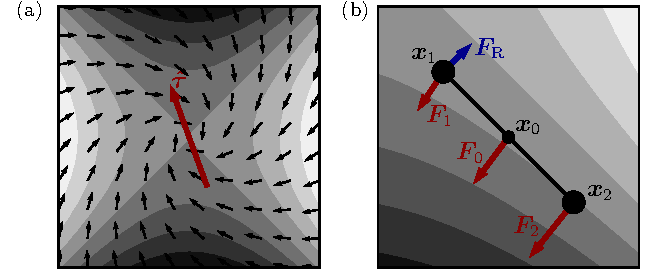
\includegraphics{single-ended.pdf}
  \caption{\label{fig:lm-singleended}
    (a) The effect of $\bm{\hat{\tau}}$ on the climbing image force in the vicinity of a saddle point (white is high energy, black is low).
        Here $\bm{\hat{\tau}}$ is pointing $20^\circ$ away from the optimal vertical direction, resulting in an inward spiralling force.
        The arrows show only the direction of the force.
    (b) The forces used to rotate a dimer, including the downhill forces on each state, $\bm{F}_i$, and the rotational force applied to state 1 about the midpoint, $\bm{F}_\mathrm{R}$.
  }
\end{figure}


\subsection{Climbing image}
The climbing image method \cite{Henkelman2000a,E2007} is perhaps the most simple single-ended method.
It involves minimising the energy of a state, but the gradient is inverted in a chosen direction, $\bm{\hat{\tau}}$, resulting in a driving force of the form,
\begin{equation}
  \bm{F} = - \grad E + 2 (\grad E \cdot \bm{\hat{\tau}}) \bm{\hat{\tau}}.
  \label{eq:lm-ci-force}
\end{equation}
An example of this force about a saddle point is shown in \cref{fig:lm-singleended}(a).

Because the gradient has been modified, this can no longer be considered a minimisation problem.
Therefore, optimisation methods that ensure that the energy decreases, such as line search, can not be used here.
This is also the case for most of the other energy landscape methods.

The climbing image is able to reach the TS so long as it starts sufficiently close to it and $\bm{\hat{\tau}}$ is approximately the direction of negative curvature at the TS.
If not, this method is likely to diverge.
Therefore, this method is often used in conjunction with other methods, especially pathway methods, in order to refine an initial estimate for the transition state, but it cannot usually locate a TS from a minimum.


\subsection{Eigenvector-following}
Unlike the climbing image method which requires the maximisation direction to be provided, the eigenvector-following method \cite{Cerjan1981,Munro1999} instead calculates it by finding the eigenvector with the lowest eigenvalue of the Hessian matrix, $\mathrm{H}$.
Also, because this direction is updated at each step, the state does not need to be initialised close to the TS.
The original method by Cerjan and Miller \cite{Cerjan1981} required calculating the inverse Hessian matrix, with later methods finding ways around the costly matrix inversion \cite{Wales1994}.
Munro and Wales then introduced the hybrid eigenvector-following method that did not require the Hessian matrix to be calculated at all, making it useful for large systems \cite{Munro1999}.

The method used by hybrid eigenvector-following to find the smallest eigenvalue is to first consider the following function for a vector $\bm{y}$,
\begin{equation}
  \lambda(\bm{y}) = \frac{\bm{y}^\mathrm{T} \mathrm{H} \bm{y}} {\bm{y}^2}.
\end{equation}
When this function is minimised with respect to $\bm{y}$ it will give the value of the smallest eigenvalue, $\lambda_\text{min}$, and $\bm{y}$ will be in the direction of the corresponding eigenvalue, $\bm{\hat{e}}_\text{min}$.
To do this without knowledge of the Hessian, $\lambda(\bm{y})$ is approximated using the function,
\begin{equation}
  \lambda(\bm{y}) \approx \frac{E(\bm{x}_0 + \delta\bm{y}) + E(\bm{x}_0 - \delta\bm{y}) - 2 E(\bm{x}_0)} {(\delta \bm{y})^2},
\end{equation}
where $\bm{x}_0$ is the position where we are evaluating the Hessian, and $\delta$ is a very small value.

Once the minimum eigenvalue and eigenvector have been found the state is stepped uphill along the eigenvector with a step size of
\begin{equation}
  h = \frac {2F} {\abs{\lambda_\text{min}} (1 + \sqrt{1 + 4 F^2 / \lambda_\text{min}^2})},
\end{equation}
with
\begin{equation}
  F = \grad E \cdot \bm{\hat{e}}_\text{min}.
\end{equation}
Then the energy is minimised along the hyperplane orthogonal to $\bm{\hat{e}}_\text{min}$.
This entire process is repeated, first finding the eigenvector then stepping uphill and minimising, until it converges to the saddle point.


\subsection{Dimer method}
The dimer method \cite{Henkelman1999,Heyden2005,Kastner2008} is a variant of the eigenvector-following method, that identifies the smallest eigenvector of the Hessian using a pair of close-lying states.
It does this by using the gradient on each state to generate a torque that turns the dimer to minimise the curvature.

By considering a close pair of states $\bm{x}_1$ and $\bm{x}_2$ with midpoint $\bm{x}_0$, each experiencing a force $\bm{F}_i = \grad E(\bm{x}_i)$ (as demonstrated in \cref{fig:lm-singleended}(b)), the rotational force applied to state 1 is found to be
\begin{equation}
\begin{aligned}
  \bm{F}_\mathrm{R} &= (\bm{F}_1 - \bm{F}_2) - [(\bm{F}_1 - \bm{F}_2) \cdot \bm{\hat{\tau}}] \bm{\hat{\tau}}\\
                    &= 2(\bm{F}_1 - \bm{F}_0) - 2[(\bm{F}_1 - \bm{F}_0) \cdot \bm{\hat{\tau}}] \bm{\hat{\tau}},
\end{aligned}
\end{equation}
where $\bm{\tau} = \bm{x}_1 - \bm{x}_0$.
This has been re-expressed using the force at the midpoint, because this is needed for the translation step, so one fewer gradient calculation is necessary.
This rotation force can be used to iteratively reorient the dimer until it reaches convergence.

Once this has occurred the dimer proceeds similarly to the climbing image method, maximising in the direction of the gradient while minimising in other directions using \cref{eq:lm-ci-force}.
However, if the dimer is located in a convex region where the curvature along the dimer is positive (such as close to minima) a different force is instead used to ensure that it does not get trapped:
\begin{equation}
  \bm{F} = (\grad E \cdot \bm{\hat{\tau}}) \bm{\hat{\tau}}.
\end{equation}



\section{Double-ended transition state methods}\label{sec:lm-de}
If both endpoints of a transition are known then single-ended methods are inadequate because they are not guaranteed to find the correct TS.
Instead, double-ended methods that converge towards the saddle from either side can be used.
Unlike pathway methods these do not typically require an initial estimate for the pathway, simplifying the process for applications with complex non-linear pathways.

There are a number of such methods, including the method introduced by Dewar, Healy, and Stewart (DHS) \cite{Dewar1984}, the step and slide method \cite{Miron2001}, the ridge-walking method \cite{Ionova1993}, and the double-ended surface walking method \cite{Zhang2013}.
Here we will focus on the first two.


\subsection{DHS method}
The DHS method \cite{Dewar1984} involves individually minimising each of the two states under a constant separation from the other state.
This separation is then steadily reduced until the method converges to the transition state.

Each iteration of the method involves first identifying which of the two states has the lowest energy.
This state is typically further from the transition state, so it is chosen to be minimised.
It is then brought towards the other, typically by about 5\%, and minimised under a fixed separation constraint.
After one or more iterations, this state gains a higher energy than the other and the minimisation switches to the other state.
The behaviour of this method is demonstrated in \cref{fig:lm-doubleended}.


\subsection{Step-and-slide method}
The step and slide method \cite{Miron2001} is similar to the DHS method, although, the roles are switched.
Instead of fixing the separation and minimising the energy, the separation is minimised at constant energy.
This is iteratively performed using a two-step process.
First, an energy is first chosen and the two states are `stepped' directly towards one another until they reach the isosurface for this energy.
Then, the states `slide' along this isosurface until the separation is minimised.
If the chosen energy is below that of the transition state then the two states will approach the TS.
Whereas, if it is too high, the states will meet and should be reverted back to their previous positions.
In this way, step and slide is able to provide an energy bound for the transition state.

In order to slide along the isosurface a bespoke minimisation procedure is required.
It must also be implemented in such a way that one state cannot accidentally jump over the saddle point, otherwise the method will fail.
For example, this may occur if the state is moved tangentially to the isosurface when close to the saddle.
Therefore, the approach used in ref.~\citenum{Miron2001} is to instead move one state downhill slightly according to the gradient and then step back up to the isosurface.
This is alternatively performed on each state until the separation has converged.

In order to choose the target energy for each iteration $E_\text{trial}$, the method uses maximum and minimum bounds for the transition state energy.
The minimum energy is given by the energies of the two states $E_{1,2}$, while the maximum energy, $E_\text{max}$, is updated any time the states combine after the slide.
Then the target energy can be chosen according to a binary search, $E_\text{trial} = (E_{1,2}+E_\text{max})/2$.
To initialise the method the maximum bound can be set by finding the maximum energy of a linear interpolation.
However, if the result is very large, it may be better to increase the energy by a set amount until an upper bound is found that way.

\begin{figure}[htb]
  \centering
  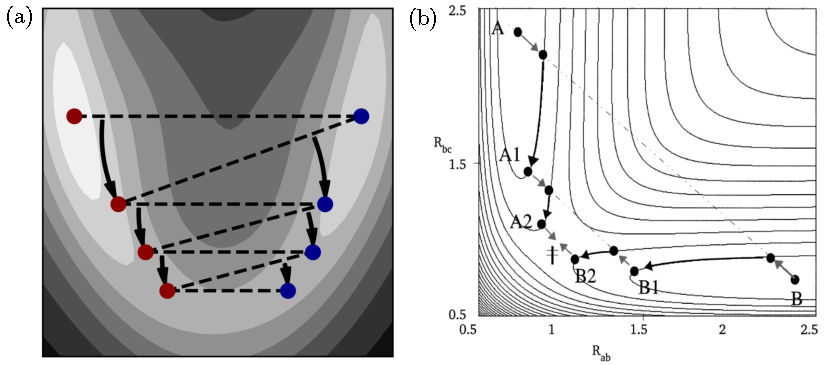
\includegraphics{double-ended.pdf}
  \caption{\label{fig:lm-doubleended}
    (a) A diagram demonstrating the behaviour of the DHS method.
    (b) An illustration of two iterations of the step and slide method.
        Adapted with permission from \cite{Miron2001}.
  }
\end{figure}



\section{Pathway methods}\label{sec:lm-pathway}
Once transition states have been identified, the full MEPs can be found by performing a downhill minimisation from either side of the saddle to the minima and tracking the trajectory.
To accurately follow the steepest descent, the step size of this minimisation should not be too large, and ideally a gradient descent method should be used.
However, other minimisation methods, such as L-BFGS, can give an approximation of the pathway, particularly for large and complex systems where gradient descent may be slow.

Alternatively, there are a number of commonly used methods that can directly find MEPs between two end points.
Each of these approaches utilise a chain of states $\lbrace \bm{x}_1, ..., \bm{x}_N \rbrace$, where each state contains a full set of system coordinates.
This chain can be initialised as a linear interpolation between the two end states, but for some systems more complex pathways may be required \cite{Ionova1993,Chu2003,Wales2012a}.
The energy of the chain is then minimised while keeping the states equally separated until it converges to the MEP.
Convergence is satisfied when the gradient orthogonal to the local pathway tangent vector goes to zero for every state in the chain,
\begin{equation}
  \grad^\perp E(\bm{x}_i) = \grad E(\bm{x}_i) - (\bm{\hat{\tau}} \cdot \grad E(\bm{x}_i)) \bm{\hat{\tau}},
\end{equation}
where $\bm{\hat{\tau}_i}$ is the tangent vector to the pathway at image $\bm{x}_i$ along the chain.

These methods are also often used in order to find the approximate locations of transition states, which occupy local maxima along the MEP.
While these methods generally do not precisely find these transition states, they can be used in conjunction with a single-ended TS search method for this purpose.

A number of pathway search methods have been proposed, although here we will focus on two commonly used approaches: the nudged elastic band (NEB) and string methods, as well as some of their variants.

\begin{figure}[htb]
  \centering
  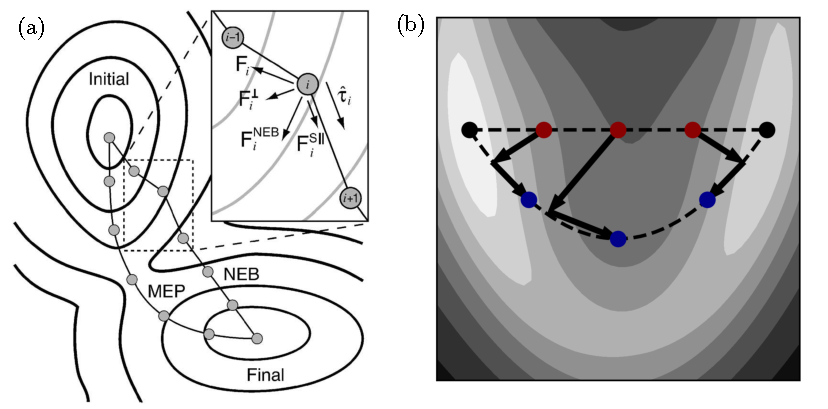
\includegraphics{pathway.pdf}
  \caption{\label{fig:lm-pathway}
    (a) A diagram showing how NEB converges to the MEP for a 2D landscape.
        The inset shows a schematic of the forces on an state in the chain.
        Adapted with permission from \cite{Sheppard2008}.
    (b) A schematic illustrating how the string method evolves.
        The arrows show the partial minimisation followed by a reparametrisation along the new interpolation.
  }
\end{figure}


\subsection{Nudged elastic band method}\label{sec:lm-neb}
The core feature of NEB methods \cite{Henkelman2000,Trygubenko2004} are that the states are kept separated along the chain using elastic spring interactions.
Therefore, the aim of the method can be considered to minimise the following total energy of the string,
\begin{equation}
  E_\text{NEB} = \sum_{i=1}^N \left[ E(\bm{x}_i) + \frac{1}{2} k \sum_{j=i+1}^N |\bm{x}_i - \bm{x}_j|^2 \right],
  \label{eq:lm-neb-energy}
\end{equation}
where $k$ is a parameter for the spring constant between the states.
However, a couple of modifications (`nudges') to the gradient of \cref{eq:lm-neb-energy} are made to reduce unwanted interference between the two contributions.
Firstly, the gradient of the underlying potential is projected perpendicular to the tangent vector, $\bm{\hat{\tau}}_i$.
This prevents the images from sliding down the pathway and ensures that the potential does not affect the parametrisation of the path, only its course.
The second modification aims to reduce the corner cutting around bends in the pathway by using only the component of the spring force parallel to the tangent vector.
Therefore the total gradient on state $i$ in the chain is
\begin{equation}
  \bm{G}_{\text{NEB},i} = \grad^\perp E(\bm{x}_i) + \bm{G}_{\text{S},i}^\parallel,
  \label{eq:lm-neb-gradient}
\end{equation}
where
\begin{gather}
  \bm{G}_{\text{S},i}^\parallel = (\bm{\hat{\tau}}_i \cdot \bm{G}_{\text{S},i}) \bm{\hat{\tau}}_i\\
  \bm{G}_{\text{S},i} = k (\bm{x}_{i+1} + \bm{x}_{i-1} - 2\bm{x}_i).
\end{gather}

The tangent vector at each point can be computed in a few ways.
The simplest approach is to use central difference between the points and normalise the result,
\begin{equation}
  \bm{\hat{\tau}_i} = \frac{\bm{x}_{i+1} - \bm{x}_{i-1}} {\abs{\bm{x}_{i+1} - \bm{x}_{i-1}}}.
\end{equation}
However, an approach that provides better results in areas of high curvature is to bisect the tangents given by forward and backward difference \cite{Henkelman2000},
\begin{equation}
  \bm{\tau}_i = \frac{\bm{x}_{i+1} - \bm{x}_{i}} {\abs{\bm{x}_{i+1} - \bm{x}_{i}}} +
                \frac{\bm{x}_{i} - \bm{x}_{i-1}} {\abs{\bm{x}_{i} - \bm{x}_{i-1}}}
  \quad\text{and}\quad
  \bm{\hat{\tau}}_i = \frac{\bm{\tau}_i}{\abs{\bm{\tau}_i}}.
  \label{eq:lm-neb-taubisect}
\end{equation}

A variant of NEB known as the doubly-nudged elastic band method (DNEB) brings further improvements to the method \cite{Trygubenko2004}, and has since seen widespread use.
This improves stability by introducing an additional term to the NEB gradient, \cref{eq:lm-neb-gradient}, such that the perpendicular component of the spring force is not completely removed.
This correction term is
\begin{equation}
  \bm{G}_\text{S}^* = \bm{G}_\text{S}^\perp - (\bm{G}_\text{S}^\perp \cdot \grad^\perp E) \grad^\perp E.
\end{equation}

The states along the chain in NEB and DNEB are unlikely to provide a particularly accurate approximation to the transition state, especially if there is significant corner cutting due to the spring interaction.
Therefore they are often used in hybrid methods with single-ended transition search methods, such as climbing image \cite{Henkelman2000a}, or eigenvector-following \cite{Trygubenko2004}.
Once the chain has converged these can be run from the highest energy state, or, can be applied to the highest state at the same time as the elastic band is minimised.
The latter requires some extra care because it is possible for the climbing state to diverge if it starts too far from the transition state.


\subsection{String method}\label{sec:lm-string}
The string method \cite{E2002,E2007} shares many similarities with NEB, however it differs essentially by the process that keeps the states separated along the chain.
Instead of using a spring force, the states are reparameterised along the pathway occasionally throughout the minimisation.

In the originally proposed method \cite{E2002} the states in the chain are driven downhill according to the gradient of the potential orthogonal to the direction of the chain.
Explicitly, for state $i$ along the chain this driving force would be,
\begin{equation}
  \bm{F}_i = - \grad E_i + (\bm{\hat{\tau}}_i \cdot \grad E_i) \bm{\hat{\tau}}_i.
\end{equation}
In a later modification to the method \cite{E2007} this driving force was simplified to remove the orthogonal projection because the reparametrisation step makes this unnecessary, leaving $\bm{F}_i = - \grad E_i$.
The tangent vector can be simply computed according to the difference between the neighbouring states, $\bm{\hat{\tau}}_i = (\bm{x}_{i+1} + \bm{x}_{i-1}) / |\bm{x}_{i+1} + \bm{x}_{i-1}|$.

After a certain number of minimisation iterations have passed the states must be reparametrised along the chain.
A suitable choice for this depends upon the system and the minimisation algorithm.
This reparametrisation may be performed using either a linear, or a cubic-spline interpolation along the set of points.
Then the new points can be equally separated along the interpolation.
The number of these new points does not necessarily need to be same as the previous step, which can make it easy to refine the pathway over time.
Additionally, the points do not need to be evenly distributed, and could instead be clustered close to the transition state by weighting the length of the interpolated path according to the local value of the potential \cite{E2007}.

Similar to NEB it is possible to use a hybrid method with climbing image \cite{E2007} or eigenvector-following in order to accurately find the transition state.
In this case, the state with the highest energy using the chosen method and should be left out of the reparametrisation step.
Another climbing image / string method hybrid, called the climbing string method, has also been proposed \cite{Ren2013}.
However, unlike the other methods, this is a single-ended saddle point search method.
This uses the string of states to guarantee that it has not left the basin of attraction for a minimum rather than for locating a MEP.


\section{Methods comparison}
\subsubsection{Minimisation}
\begin{table}
  \begin{tabularx}{\textwidth}{lCCCCC}
    \hline\hline
    Method              & Local  & Global & Gradient & Hessian & Ensemble\\
    \hline
    Gradient descent    & \cmark & \xmark & \cmark   & \xmark  & \xmark\\
    L-BFGS              & \cmark & \xmark & \cmark   & \xmark  & \xmark\\
    FIRE                & \cmark & \xmark & \cmark   & \xmark  & \xmark\\
    Newton's method     & \cmark & \xmark & \cmark   & \cmark  & \xmark\\
    Simulated annealing & \cmark & \cmark & \xmark   & \xmark  & \xmark\\
    Basin hopping       & \xmark & \cmark & \cmark   & \xmark  & \xmark\\
    Genetic algorithm   & \xmark & \cmark & \xmark   & \xmark  & \cmark\\
    \hline\hline
  \end{tabularx}
  \caption{
    A comparison of the different minimisation methods, indicating which can be used as local or global minimisers, which require the gradient or the Hessian, and which use an ensemble of states.
  }
\end{table}
Minimisation methods that use the Hessian, like Newton's method, generally provide faster convergence compared to other methods.
However, the calculation of the Hessian can become the limiting factor if the number of degrees of freedom is large, which it generally is in the continuous systems that we are interested in.
Since L-BFGS is quasi-Newtonian, it benefits from this faster convergence without being bogged down by the calculation of the Hessian, therefore it is ideal for our purpose.

FIRE is also a good option with convergence speeds approaching that of L-BFGS \cite{Bitzek2006}, so it is a good alternative for cases where L-BFGS has difficulty.
It is also more amenable to parallelisation along the degrees of freedom, because there are much fewer vector magnitudes and dot products calculated per iteration compared to L-BFGS.
On the other hand, FIRE has a free parameter, the maximum time step, which can require some tuning for each system and makes the method a little more difficult to use.

As for simulated annealing, it is primarily a global minimiser, but it can also be used to find local minima.
Compared to L-BFGS and FIRE it converges much more slowly, and the random perturbations make it possible to jump into the basin of another minima.
Therefore, where possible other methods should be used, but it is particularly useful if the gradient cannot be calculated or is undefined.

However, when it comes to global optimisation or locating multiple minima, basin hopping and the genetic algorithm tend to win out.
For genetic algorithm, the ensemble of states provides a much larger accessible search region, resulting in better performance for most problems \cite{Sexton1999,Kerr2019}.
Furthermore, it is well suited to parallelisation because each state can be run separately, with a minimal number of interactions in each generation.
As for basin hopping, it is particularly attractive because of its simplicity, the only variable parameter being the temperature.
This makes it more straightforward to apply to new systems in comparison to simulated annealing or genetic algorithm, which depend heavily upon the choice of cooling schedule and genetic operators, respectively, as well as their related parameters.

\subsubsection{Transition states and pathways}
\begin{table}
  \begin{tabularx}{\textwidth}{lCCCCC}
    \hline\hline
    Method          & Number of states & TS from endpoints & Can find multiple TS & No interpolation\\
    \hline
    Single-ended TS & 1                & \xmark            & \xmark               & \cmark \\
    Double-ended TS & 2                & \cmark            & \xmark               & \cmark \\
    Chain-of-states & $\ge 3$          & \cmark*           & \cmark*              & \xmark \\
    \hline\hline
  \end{tabularx}
  \caption{
    A comparison of the three types of TS and pathway methods, including the number of states that are optimised, if the method can find one or multiple TS between two chosen endpoints, and if an interpolation is required.
    An asterisk indicates a hybrid method is required.
  }
\end{table}
Single-ended search methods are generally efficient at locating saddle points quickly.
This makes them particularly well suited for surveying large numbers of transition states or refining estimates, such as those obtained from chain-of-states methods.
However, if a specific pathway between two known end states is of interest, single-ended methods are often inadequate and double-ended methods and chain-of-states methods should be used instead.

The simplicity of the climbing image method makes it excellent for refining transition state estimates, but it cannot usually be started far from the transition state, such as from minima.
The requirement for a tangent vector estimate also restricts its use.
The eigenvector-following and dimer methods solve these issues and can be used in most situations, but their success depends strongly upon the number of iterations allowed when calculating the uphill direction and the corresponding convergence criteria.
This can also take some time to adequately converge for large numbers of degrees of freedom.
If there are zero eigenmodes of the Hessian, such as global translation and rotation, then the dimer and eigenvector-following methods can also struggle and special consideration is required.

For finding the transition states and pathways between two end points, the choice between using double-ended transition state methods or chain-of-state methods will depend upon the situation.
Chain-of-states methods will be preferable if full pathways are desired, or precise transition states are not required.
Likewise, if there are many intermediate minima and transition states, which is often the case for particulate systems, chain-of-states methods can identify the approximate locations for many of these at once.
Chain-of-states methods are also more reliable, whereas double-ended methods can often fail to locate a transition state.
As a result, chain-of-states methods are much more widely used than other methods.
However, double-ended bracketting methods can be particularly efficient for finding transition states for pathways with no (or very few) intermediate minima.
This is especially true if the pathways are highly non-linear on the landscape, where chain-of-states methods require a large number of images to accurately approximate the pathway.
It can also make it difficult to choose an appropriate initial pathway estimate, which is necessary for chain-of-states methods.
These advantages make double-ended methods attractive for elastic structures and other continuous systems, which have comparatively few minima, yet complex, non-linear pathways.

Comparing the double-ended TS methods, we find that each has different advantages and disadvantages.
The DHS method is particularly simple to implement and use, and it can be good for obtaining the TS within a certain distance error.
However, because only one state is minimised at a time, the distance must be reduced quite slowly for it not to pass over the ridge.
As for the step and slide method, it is useful for getting a bound on the energy of the transition state.
However, the minimisation along a constant energy surface requires a more complicated implementation that is not as efficient as standard minimisation algorithms.
Also, it can be hard to know how much to initially increment the energy, if it is too large or too small the method may take a lot longer to converge.

Of the pathway methods, both DNEB and string methods have a comparable effectiveness.
Each can be advantageous for different systems and sets of parameters, but it is difficult to know which will be better a priori \cite{Koslover2007}.

  \chapter{Binary Image Transition State Search}
\label{ch:bitss}
\graphicspath{{bitss/fig/}}


\section{Introduction}
Transition states are central to the description of reconfiguration mechanisms for systems in chemistry, condensed matter physics, and engineering.
Historically, many computational methods for locating transition states have grown from an atomistic or particulate perspective.
These have proven to be important tools for understanding, for example, protein folding \cite{Bryngelson1995,Onuchic1997}, biological and industrial catalysis \cite{Boehr2006,Kerns2015,Guo2018a}, quantum tunnelling \cite{Richardson2016,Vaillant2019}, crystallisation \cite{Richard2018}, and cluster formation \cite{Wales1998,Wales2012}.

More recently, it is increasingly being recognised that transition states are useful in mesoscale or macroscale systems.
Here, the minimum energy barriers provide important lower bounds to the energy input required for transitions to occur.
This has been used to understand failure in structural engineering applications \cite{Panter2019,Hutchinson2018}, for the development of super liquid-repellent surfaces \cite{Zhang2014,Panter2019a,Amabili2017}, and investigating locomotion through complex terrain for robotics \cite{Othayoth2020}.
Moreover, it is becoming desirable to tailor elastic deformation transitions to enable technologies such as advanced deployable structures \cite{Filipov2015,Zhai2018}, mechanical sensors and actuators \cite{Bertoldi2017,Truby2016,Chi2022,Bonfanti2020}, and energy absorbers \cite{Shan2015,Giri2021} to name but a few.

As discussed in \cref{sec:lm-se,sec:lm-de,sec:lm-pathway}, transition state search methods generally fall into two categories, single- and double-ended methods.
Single-ended methods are initialised at a single state and attempt to climb to a nearby saddle point.
Examples include eigenvector following \cite{Cerjan1981}, the dimer method \cite{Heyden2005,Kastner2008,Zhang2016}, and climbing image methods \cite{E2007,Ren2013}.
Double-ended methods can be further subdivided into two groups.
The first are bracketing methods, which involve two states converging to the transition state from either side.
These include the Dewar-Healy-Stewart (DHS) algorithm \cite{Dewar1984}, ridge method \cite{Ionova1993}, the step and slide method \cite{Miron2001}, and the double-ended surface walking method \cite{Zhang2013}.
The second group utilise chain-of-states methods for finding pathways, such as string method \cite{E2002,E2007} and doubly-nudged elastic band (DNEB) \cite{Trygubenko2004}.
In order to locate transition states, these are combined with single-ended methods, resulting in a hybrid approach.
However, chain-of-states methods require an appropriate initial interpolation, which can sometimes be challenging to obtain \cite{Wales2012a}.

Unfortunately, a large range of landscapes prove challenging or impossible to explore via these methods.
One such problem arises from the push towards larger and more complex systems \cite{Trefethen2013,Shalf2020,Alexander2020}, resulting in the need to develop algorithms that are more computationally and memory efficient, and can incorporate optimisation strategies such as on-the-fly adaptive remeshing and coarse-graining.
These typically involve changing the resolution or discretisation of the systems to focus the computational time on important regions, such as using a higher resolution mesh in regions of high stress in finite element simulations \cite{Lee1994}.
However, chain-of-states methods involve a coupling between the configurations of each state, and so there is an issue if they have different discretisations and numbers of degrees of freedom.
Meanwhile, single-ended methods can be inefficient because they are not well suited for identifying specific pathways and can spend a large amount of time searching for undesired transition states.
Another major challenge in studying complex energy landscapes relates to the presence of locally flat or discontinuous regions, such as when considering patchy \cite{McMullen2018,Nguemaha2018,Chen2018b} and hard-body \cite{Richard2018,Santra2018} interactions in atomistic simulations, systems of polymer chains \cite{Mokkonen2016}, or collision constraints for macroscopic objects \cite{Wriggers2006}.
Flat zero-modes in the landscape pose issues for single-ended search methods and current bracketing methods that rely only upon local information.
Specialist treatment can sometimes be used such as in the case of global rotation and translation \cite{Page1988}, but they are thwarted by local zero-modes.
Finally, current methods cannot typically be applied in the case of discontinuous potentials, or if the gradient is prohibitively expensive to compute, because continuous, differentiable optimisation functions are required.

In this chapter we introduce a new double-ended bracketing method, the Binary-Image Transition State Search (BITSS).
Using a range of different applications, we demonstrate that it successfully addresses each of the above challenges.
In addition, we show that BITSS is superior compared to existing bracketing methods, allowing us to access the transition states when other methods fail.


\section{BITSS method}
The method begins by first initialising the states, $\bm{x}_1$ and $\bm{x}_2$, in the basins of attraction of different local minima, such as the two blue spots in the 2d potential in \cref{fig:bitss-toy2d}(a).
These can be set to the minima, but this is not a necessary requirement.
The energies of these two states are then minimised, while constraining their separation.
This is iteratively reduced to zero, such that, at iteration $i$, their separation is
\begin{equation}\label{eq:bitss-diteration}
  d_i = (1 - f) d_{i-1},
\end{equation}
with $d_0$ taking the value of the separation between the two initial states.
A reduction factor of $f = 0.5$ is successful for most applications, but this can be made smaller to ensure that the states do not slide off the ridge between the two basins of attraction.
This and other parameters in this chapter are listed in \cref{tab:bitss-params}.
Different metrics may be used to compute this distance, although we will simply use the Euclidean distance,
\begin{equation}
  d(\bm{x}_1, \bm{x}_2) = \sqrt{\sum_i (x_{1,i} - x_{2,i})^2}.
\end{equation}
To further ensure that neither state is pulled over the ridge, a secondary constraint enforces equal energies for the two states.
Using this strategy, the two states will meet at the lowest point on the ridge, the transition state.

The two constraints are implemented using energy penalty terms, which result in driving forces on the two states if the constraints are not met, such as in \cref{fig:bitss-toy2d}(b).
Including these energy penalty terms gives the total BITSS energy for the pair of states,
\begin{equation}\label{eq:bitss-e}
  E_\mathrm{BITSS}(\bm{x}_1, \bm{x}_2) = E_1 + E_2
    + \kappa_e \left( E_1 - E_2 \right) ^2
    + \kappa_d \left( d(\bm{x}_1, \bm{x}_2) - d_i \right) ^2,
\end{equation}
where $E_1$ and $E_2$ are the single-state energies, and $\kappa_e$ and $\kappa_d$ parametrise the strengths of the energy and distance constraints.

The L-BFGS algorithm is chosen to minimise this energy, owing to its fast convergence and low memory requirement for large numbers of degrees of freedom \cite{Liu1989}.
However, any other minimisation method can be used in practice.


\subsection{Choosing the constraint coefficients}\label{sec:bitss-coefficients}
To ensure that the transition state is located successfully, the constraint strengths $\kappa_d$ and $\kappa_e$ are updated as the algorithm proceeds using information from the system.
These are initially calculated at the start of each minimisation, and regularly recalculated throughout (once per 100 iterations is used here).
These are set such that the driving forces due to the constraints and single-state energies are of similar size, in order to prevent the constraints from dominating the underlying potential or causing large jumps that make a state pass over the ridge.

To obtain the expression for the energy coefficient, $\kappa_\text{e}$, we first assume that the separation is fixed, so the distance term can be ignored.
The coefficient $\kappa_\text{e}$ must be high enough to prevent one state from being pulled over the ridge, for which the greatest risk occurs when the gradient on one state is much greater than the other, e.g. $\abs{\grad E_2} \gg \abs{\grad E_1}$.
In this case the total gradient is approximated by
\begin{equation}
  \grad E_\text{BITSS} = \left[ 1 - 2 \kappa_\text{e} (E_1 - E_2) \right] \grad E_2.
\end{equation}
Therefore, when not at a transition state or a minimum in the landscape ($\abs{\grad E_2} \neq 0$) convergence will occur when the term in the square brackets is zero, resulting in $E_1 - E_2 = 1 / 2 \kappa_\text{e}$.
This energy difference should be less than current energy barrier, so we can substitute it with $E_\text{B} / \alpha$, where $\alpha$ is a constant greater than one, and $E_\text{B}$ is an estimation for the current energy barrier, evaluated using a linear interpolation between the two states.
This leaves us with an expression for $\kappa_\text{e}$.
\begin{equation}
  \kappa_e = \frac {\alpha} {2 E_\mathrm{B}}.
  \label{eq:bitss-ke}
\end{equation}

The distance coefficient is determined by assuming that the energies are equal and thus the energy constraint can be ignored.
In this case, convergence will occur when $\grad E_1 + \grad E_2 = -2 \kappa_\text{d} (d - d_i) \grad d$.
It is then possible to find the value of $\kappa_\text{d}$ for which the magnitude of each side of this equation is equal for a desired relative error in the distance, $\beta = (d - d_i) / d_i$,
\begin{equation}
  \kappa_\text{d} = \frac {\sqrt{\abs{\grad E_1}^2 + \abs{\grad E_2}^2}} {2 \sqrt{2} \beta d_i}.
\end{equation}
Here, it has been used that the gradient of the distance with respect to a single state has a magnitude of 1, so the total magnitude for the pair of states is $\abs{\grad d} = \sqrt{1^2+1^2} = \sqrt{2}$.
To ensure that the coefficient is not too small if the gradient is close to zero, such as when the states are initialised at the minima, a lower bound is set by replacing $\abs{\grad E_1}$ and $\abs{\grad E_2}$ with $2 E_\text{B} / d_i$.
This results in the following overall equation for $\kappa_\text{d}$.
\begin{equation}
  \kappa_d = \max \left(
    \frac {\sqrt{\abs{\grad E_1}^2 + \abs{\grad E_2}^2}} {2\sqrt{2} \beta d_i} \; , \;
    \frac{E_\mathrm{B}}{\beta d_i^2} \right),
  \label{eq:bitss-kd}
\end{equation}

In practice, when numerically minimising, the states will jump about slightly which can result in large gradients perpendicular to the optimal movement direction.
To reduce this effect, the gradients used in \cref{eq:bitss-kd} are projected in the direction of the separation between the two states:
\begin{equation}
  \abs{\grad E_n} \approx \frac {\abs{(\bm{x}_1 - \bm{x}_2) \cdot \grad E_n}} {\abs{\bm{x}_1 - \bm{x}_2}}.
\end{equation}

In order to choose suitable values for the constant parameters $\alpha$ and $\beta$ we have tested different parameter choices using the seven-particle cluster and cylindrical buckling examples, described in \cref{sec:bitss-systems}.
These are used with a fractional separation decreases of $f=0.5$ and $f=0.4$, respectively.
\Cref{fig:bitss-paramtest} shows which choices lead to convergence and the speed at which this occurs.

\begin{figure}[htb]
  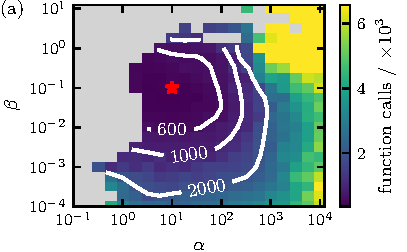
\includegraphics{paramtest-a.pdf}%
  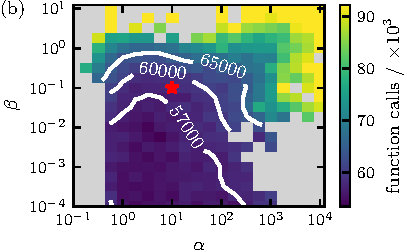
\includegraphics{paramtest-b.pdf}%
  \caption{\label{fig:bitss-paramtest}
    Speed of convergence of the BITSS method under different choices of parameters for (a) the seven-particle cluster, and (b) cylindrical buckling.
    The speed is given by the number of evaluations of the gradient until the two states are separated by less than a thousandth of the initial separation.
    The combinations that do not converge to the transition state are shown in grey.
    The chosen parameters are marked by a red star.
  }
\end{figure}

The parameters $\alpha = 10$ and $\beta = 0.1$ are chosen for converging quickly, while remaining far from the regions of non-convergence in both test cases.
Hence, this choice is likely to still succeed even if the boundaries of the non-convergence region shifts when using different systems.
However, these parameters may also be adapted to a specific system if desired.


\subsection{Method summary}
In summary, the BITSS method involves iteratively performing the following three steps:
\begin{enumerate}[noitemsep,nolistsep]
  \item Reduce the constrained separation, according to \cref{eq:bitss-diteration}.
  \item Minimise the potential of the pair of states, \cref{eq:bitss-e}.
  \item Recompute the constraint coefficients, $\kappa_e$ and $\kappa_d$, at regular intervals using \cref{eq:bitss-ke,eq:bitss-kd}.
\end{enumerate}
This process is completed once a suitable convergence criterion is reached.
This can either be based upon the separation between the states, the size of gradient at the midpoint between them, or the change in the position of the midpoint.

Using this approach, the typical trajectories of the states are demonstrated for a simple 2D potential in \cref{fig:bitss-toy2d}(a).
Initially, the lower energy state jumps up to satisfy the equal energy constraint and then moves to minimise the separation without increasing its energy.
Then, the two states converge directly towards one another, before being deflected towards the saddle in the ridge.
Consequently, if there are multiple possible pathways between two states, BITSS will be biased towards identifying those that are more direct or with lower energy.
Furthermore, the final two states are positioned either side of the transition state in the direction of the negative curvature eigenvector, $\bm{\hat{\tau}}$ (\cref{fig:bitss-toy2d}(c)).
So, BITSS automatically identifies the `reactive mode' and associated eigenvalue in addition to the transition state.
Once the transition state has been identified, it is possible to find the full minimum energy pathway by tracing the trajectory of downhill minimisations from the two final states, which are either side of the saddle.

\begin{figure}[htb]
  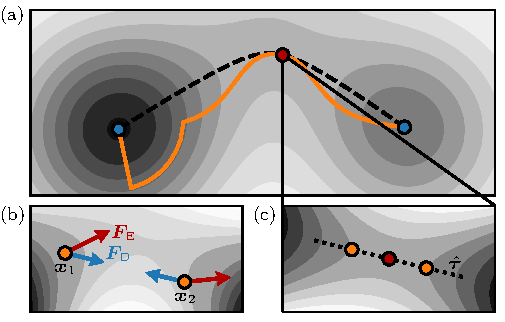
\includegraphics{toy2d.pdf}
  \caption{\label{fig:bitss-toy2d}
    Schematics of the BITSS method on a simple 2D potential with two minima.
    (a) The orange line shows the trajectories of the two states from the minima (blue) to the transition states (red) under the BITSS method.
        The minimum energy pathway is shown by the dashed line.
    (b) A snapshot of the BITSS minimisation showing the driving forces on each state due to the energy constraint, $\bm{F}_\mathrm{E}$, and distance constraint, $\bm{F}_\mathrm{D}$, with $E_1 < E_2$ and $d(\bm{x}_1,\bm{x}_2) > d_i$.
    (c) The final configuration of the BITSS method showing the two states in orange, the transition state in red, and the negative curvature eigenvector, $\bm{\hat{\tau}}$.
  }
\end{figure}

In the event that there are intermediate stable states, there will be a chain of multiple transition states between the two minima.
In this case, the equal-energy constraint will not prevent the states from passing over the lower energy transition states, so BITSS should converge to the transition state with the highest energy.
This enables the identification of the overall energy barrier, providing estimates about the overall ease of the transition, or the rate for chemical processes.
However, as demonstrated later in \cref{sec:bitss-multits}, if multiple transition states have very similar energies then a smaller distance reduction factor, $f$, may be necessary to ensure that it does indeed converge to the highest transition state.
Furthermore, if all of transition states or the full pathway are desired, BITSS can be continually repeated from one of the minima downhill from the located transition state and one of the initial minima until the initial minima are piece-wise connected by a full pathway.

\subsection{Changes for undefined gradients}
In order to use BITSS in situations where the gradients are unknown a couple of alterations to the method must be made.
First, the calculation of $\kappa_d$ in \cref{eq:bitss-kd} must be adapted to avoid the use of gradients.
This can be done by simply removing the first term and just using the second term in the equation.
Secondly, L-BFGS can no longer be used because it requires knowledge of the gradients.
We must instead use a minimiser that does not require a differentiable optimisation function, for which we use simulated annealing \cite{Kirkpatrick1983}.
This has a chance of randomly jumping one state over the dividing barrier, but we can reduce this probability by limiting the initial temperature and maximum random displacement.
We typically employ $T_0 = E_\mathrm{B} / 10$, and $d_\mathrm{max} = d(\bm{x}_1, \bm{x}_2) / 100$.


\section{Details of the test systems}\label{sec:bitss-systems}
To test the BITSS method several diverse systems are used which exhibit a broad range of energy landscapes.
These are described below, and further details of the potentials can be found in \cref{sec:ell-potentials}, including the full functions for their energy and gradient.

Firstly, the 2D potentials in \cref{fig:bitss-toy2d,fig:bitss-bracketing} use a sum of Gaussian potentials, \cref{eq:bitss-gaussianpeaks}, to create a landscape with two minima and a curved pathway between them.
\begin{equation}
  E(x,y) = \sum_i a_i \exp\!\left( - \frac{(x-b_{x,i})^2}{c_{x,i}} - \frac{(y-b_{y,i})^2}{c_{y,i}} \right)
  \label{eq:bitss-gaussianpeaks}
\end{equation}
The parameters for each figure are provided in \cref{tab:toy2dparams,tab:bracketingparams}.

\begin{table}[ht]
  \begin{tabularx}{0.5\textwidth}{CCCCC}
    \hline\hline
    $a$ & $b_x$ & $b_y$ & $c_x$ & $c_y$ \\
    \hline
    -3  & -1.4  &   0   &   1   &   1   \\
    -2  &  1.4  &   0   &   1   &   1   \\
    -1  &  0.07 &   1   &   1   &   1   \\
    \hline\hline
  \end{tabularx}
  \caption{\label{tab:toy2dparams}
    Parameters for the Gaussians to produce the potential used in \cref{fig:bitss-toy2d}.
  }
\end{table}

\begin{table}[ht]
  \begin{tabularx}{0.5\textwidth}{CCCCC}
    \hline\hline
    $a$  & $b_x$ & $b_y$ & $c_x$ & $c_y$ \\
    \hline
    -1   &   0   &   0   &  10   &  10   \\
     1   &   0   &   0   &   1   &   1   \\
     5   &   2   &   0   &   1   &  0.1  \\
    -1   &   1   &   1   &  0.1  &  0.1  \\
    -1   &   1   &  -1   &  0.1  &  0.1  \\
    0.01 &   0   &   0   &   1   &   1   \\
    0.5  &  -2   &   0   &   1   &   1   \\
    \hline\hline
  \end{tabularx}
  \caption{\label{tab:bracketingparams}
    Parameters for the Gaussians to produce the potential used in \cref{fig:bitss-bracketing}.
  }
\end{table}

The next system is a two-dimensional cluster of seven particles, with 14 degrees of freedom representing the particle coordinates.
A Lennard-Jones potential is used for the interaction between each pair of particles.
This is frequently used as a test system for studying transition rates \cite{Wales2002,Passerone2001}.
The cluster has a global minimum when the particles are arranged in a hexagon, and it undergoes a transition to a second minimum when a pair of the outer particles slide past one of the other particles, as shown in \cref{fig:bitss-testsystems}(a).

The third test case is the buckling of a thin cylindrical shell under axial compression.
For this, the ends of the cylinder are compressed towards one another by 0.14\% and then fixed in place.
The characteristic transition in \cref{fig:bitss-testsystems}(b) shows the formation of a stable dimple from an initially unbuckled cylinder.
This transition is essential to capture and predict mechanical failure under strain \cite{Panter2019,Virot2017}.
This is modelled using a 2D triangular mesh to represent the surface of the cylinder, with \num{35400} degrees of freedom for the node coordinates in three-dimensional space.
The elastic energy is calculated using a bar-and-hinge model.
This treats all the bonds in the mesh as elastic springs and connects all adjacent pairs of triangles with elastic hinges in order to calculate the stretching and bending energies, respectively.

The final system is the droplet on a striped surface, with \num{40000} degrees of freedom representing the local fluid compositions at each site of the discretised domain.
The regions on the surface are hydrophilic and hydrophobic, with contact angles of $\theta_a=60\si{\degree}$ and $\theta_b=110\si{\degree}$, respectively.
In this example, the transition involves the movement of the droplet from being centred upon one of the hydrophilic regions, to straddling across two of them, as shown in \cref{fig:bitss-testsystems}(c).
Droplet transitions on patterned surfaces such as this are vital to understand as powerful bio-inspired liquid manipulation strategies \cite{Kusumaatmaja2006,Brown2016}.
The system is modelled on a $200\times200$ 2D grid (and $400\times400$ in \cref{sec:bitss-adaptive}) with a phase-field model \cite{Panter2019a}.
This uses an order parameter to represent the phase of the fluid (liquid or gas) at each point on the grid, and it varies smoothly, resulting in a diffuse interface between the phases.
This interface width is set to a value of 2.5 lattice units.
The total volume of the droplet is also constrained to ensure that it does not fully evaporate, using an energy penalty for any variation from the target volume.
Because the order parameter only varies when it is at the interface of the droplet, the transitions follow highly non-linear pathways across the model's configuration space.
Therefore, it is a useful test for how BITSS behaves for complex pathways.

\begin{figure}[htb]
  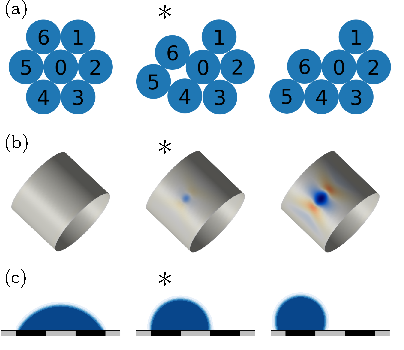
\includegraphics{testsystems.pdf}
  \caption{\label{fig:bitss-testsystems}
    Three of the transitions used to test the BITSS method.
    These are: (a) a Lennard-Jones seven-particle cluster, (b) cylindrical shell buckling, and (c) wetting of a chemically-striped surface.
    The configurations shown correspond to the two minimum energy states and the transition state, marked by an asterisk.
  }
\end{figure}


\section{Results and Discussion}
\subsection{Comparison with other bracketing methods}\label{sec:bitss-bracketing}
The BITSS potential in \cref{eq:bitss-e} and iterative steps above offer key advantages over existing bracketing methods that also use two states to locate the transition state.
For instance, in the ridge method \cite{Ionova1993}, the two images are initially chosen to bracket the largest energy point on an interpolated path between the two endpoints.
However, this is not guaranteed to be on the ridge containing the transition state, and specialist methods are required to avoid high-energy local maxima, or when the initial path contains multiple candidate maxima.
In another example, the double ended surface walking method \cite{Zhang2013} requires Gaussian bias potentials to be added at each iteration to force two dimers to climb uphill in the landscape.
For high numbers of degrees of freedom and many iterations, this becomes very computationally expensive.

The two methods most similar to BITSS are the DHS \cite{Dewar1984} and step and slide \cite{Miron2001} methods.
In the step and slide method, the separation between two images is minimised while their energy is fixed (iteratively increasing the energy up to the transition state).
Conversely in the DHS method, the energy of an image is minimised while the image separation is fixed (iteratively decreasing the separation and changing the frozen image up to the transition state).
To illustrate how BITSS is superior compared to these methods, we consider the hooked 2d potential in \cref{fig:bitss-bracketing}.
For this potential the energies of the images ascend higher than that of the transition state and consequently both of these methods fail to converge to the saddle point regardless of the parameters that are used.
The step and slide method fails in this situation because it always expects that the energy of the two states is below the saddle point if they have not converged, so it has no means of descending down the ridge.
For DHS, the images reach a certain point at which one state can pass over the ridge by minimising its energy.
At this point DHS will fail even if the distance is reduced very slowly.
In contrast, the BITSS method is successful for this potential.
This is because the combination of distance and energy constraints allow BITSS to approach a transition state from both below and above (by sliding down a ridge).

\begin{figure}[htb]
  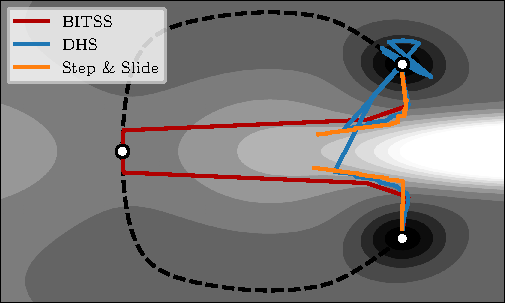
\includegraphics{bracketing.pdf}
  \caption{\label{fig:bitss-bracketing}
    Trajectories of the bracketing methods on a hooked potential with a single saddle point.
    The minimum energy pathway is shown by the dashed line.
  }
\end{figure}

Furthermore, using both an energy and distance constraint with BITSS provides improved efficiency over these methods which each use just one of the constraints.
In the case of DHS, fixing one state in place and optimising the other means that the amount that the separation is reduced must be much smaller than BITSS to ensure that it does not pass over the ridge.
Meanwhile, in step and slide, it is difficult to obtain a reasonable energy increment when the two states are far from the transition state, leading to a larger than necessary number of iterations.
Also, restricting the minimisation to a constant energy surface can result in a considerably more complex method, as the states must be constantly projected back onto this surface.


\subsection{Comparison with chain-of-states methods}
In contrast to BITSS, chain-of-states methods do not typically find transition states directly.
Instead, they are designed to find the full pathway (or an approximation thereof), and a secondary method can then be used to refine to the transition state.
As we will demonstrate, this strategy is successful for simple, linear pathways, but faces two key challenges when the pathway is highly non-linear.
Firstly, for such complex pathways, a large number of states are required to sufficiently approximate the minimum energy pathway.
The second is that choosing a suitable initial interpolation can be problematic to achieve.
BITSS can be advantageous in both these regards, as only two states are evolved, regardless of the pathway complexity, and no initial interpolation is required.

Here we compare the speeds of convergence of BITSS to two widely used approaches for finding transition states that employ chain-of-states methods: climbing image nudged elastic band (CINEB) \cite{Henkelman2000a}, and DNEB with hybrid eigenvector following (DNEB-HEVF) \cite{Cerjan1981}.
Three diverse systems are used for this comparison, the seven-particle cluster, cylindrical buckling, and wetting of a droplet on a striped surface.
For the latter, the high non-linearity of the pathway causes the chain-of-states methods to fail to find the correct pathway if they use a simple linear interpolation.
Instead, the position of a semi-circular droplet is interpolated between the two final positions.

These methods use NEB and DNEB which are described in \cref{sec:lm-neb}.
Put simply, they involve minimising the total energy of a chain of states that are connected by elastic springs to keep them equally spaced along the transition pathway.
The optimal values for these spring constants are system dependent.
They are chosen such that they keep the states equidistant without overwhelming the gradients arising from the potential energy landscapes under consideration.
We employ $10^{-1}$ for the Lennard-Jones particle cluster, $10^{-2}$ for the cylindrical buckling example, and $10^{-6}$ for the striped wetting system.
We also fix the two end-points at the minima, so the number of states that are minimised is two fewer than the number of states in the chain.

CINEB modifies NEB by altering the behaviour of the state with the highest energy.
The direction of minimisation on this state is inverted along the pathway direction, effectively converting the saddle point into a local minimum.
Alternatively, DNEB-HEVF involves first minimising the chain of states until a convergence criterion is met, and then performing hybrid eigenvector following from the highest energy state, moving uphill along the smallest eigenvector of the Hessian until it reaches the transition state.
For completeness, we also combine hybrid eigenvector following with BITSS and include the results in the convergence comparison.

When using hybrid eigenvector following, we need to set out criteria to determine when the double-ended method has sufficiently converged, at which point the eigenvector following method begins.
For BITSS, the criterion is when the average of the two states changes by less than a tenth of the reduction in the separation given by \cref{eq:bitss-diteration} during a BITSS step.
For DNEB, the root-mean-square of the total energy gradient of the chain of states is used with a convergence criterion of $10^{-3}$ for the particle cluster and cylindrical buckling systems, and $10^{-5}$ for the striped wetting.
We employ the hybrid eigenvector following method implemented in the program OPTIM \cite{OPTIM}.

It is also possible to use the string method with a climbing image \cite{E2007} or eigenvector following \cite{Zimmerman2013}; although, in this case, the results are expected to be similar to the nudged elastic band methods.
We note that our aim in this section is to observe how the BITSS method behaves for different systems, rather than providing a comprehensive comparison of the currently available methods, which has been performed in other works \cite{Koslover2007,Sheppard2008}.

\begin{table*}[tb]
  \begin{tabularx}{\textwidth}{@{}C @{} C@{}C @{} C@{}C@{}C @{} C@{}C@{}C @{}} % Remove column separators to prevent it being too wide
    \hline\hline
    \tworow{System} & \tworow{BITSS} &
      \tworow{\begin{tabular}[c]{@{}c@{}}BITSS-\\HEVF\end{tabular}} &
      \multicolumn{3}{c}{DNEB-HEVF} & \multicolumn{3}{c}{CINEB} \\
    \cmidrule(lr){4-6}\cmidrule(lr){7-9}
             &             &             & 3           & 5           &  20          & 3   & 5          & 20          \\
    \hline
    LJ-7     & 148         & 144         & 135         & 138         &  361         & 30  & 153        & 1692        \\
    Buckling & \num{12866} & \num{14446} & \num{73694} & \num{7315}  &  \num{12094} & --- & \num{8352} & \num{77904} \\
    Wetting  & \num{12100} & \num{17262} & \num{17840} & \num{17721} &  \num{48286} & --- & ---        & ---         \\
    \hline\hline
  \end{tabularx}
  \caption{\label{tab:speed}
    Number of potential gradient calculations required to reach the transition state for the three comparison examples.
    The climbing image nudged elastic band (CINEB) and DNEB with hybrid eigenvector following (DNEB-HEVF) methods have been run for different numbers of images.
    Convergence is determined to be when the root-mean-square of the gradient at the estimate for the transition state is less than $10^{-4}$.
    The fields left blank indicate that the method has not converged to the correct transition state.
  }
\end{table*}

The results for the three systems are shown in \cref{tab:speed}.
First, we note that for all three systems, using hybrid eigenvector following does not significantly improve the speed of BITSS.
Indeed, for buckling and especially wetting, HEVF is detrimental to performance.
Next, it is interesting to compare each method's performance between simple and complex pathways.
In contrast to the wetting transition's highly non-linear pathway, the pathways of the LJ-7 rearrangement and the buckling system can be simply tracked following a gradual variation in the order parameters.
For LJ-7, this is the translation of atoms 5 and 6, and for buckling, this is the radial displacement of the centre of the dimple \cite{Panter2019}.
For these simpler pathways, BITSS is generally slower, but for the complex pathway, BITSS is faster.
Moreover, we see that for the wetting example, CINEB does not converge to the transition state because the estimated tangent vector is highly inaccurate due to the non-linearity of the pathway.

For situations where memory is limited, it is important to minimise the number of images used.
However, efficiently finding the TS is challenging for both CINEB and DNEB-HEVF if too few images are used, as observed for the cylindrical buckling with three images.
BITSS, on the other hand, converges using only two images.


\subsection{Adaptive discretisation}\label{sec:bitss-adaptive}
\begin{figure}[tb]
  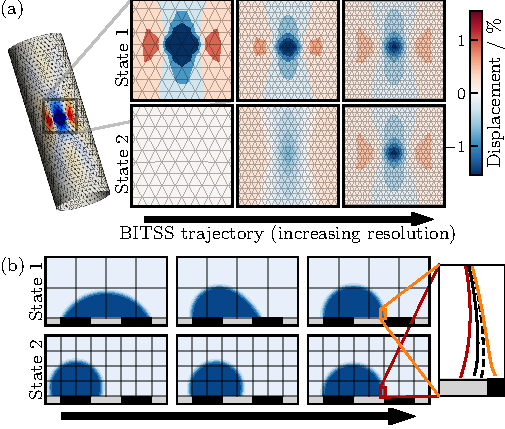
\includegraphics{adaptivemesh.pdf}
  \caption{\label{fig:bitss-adaptivemesh}
    Demonstration of BITSS addressing the challenges associated with adaptive remeshing.
    (a) Snapshots of the BITSS method for the buckling of a cylinder with a changing mesh.
        The radial displacement relative to the unbuckled cylinder is shown, as well as the underlying triangular mesh.
    (b) Snapshots for the striped wetting example with different resolutions for the two states.
        Each grid cell denotes $50\times50$ lattice nodes.
        The zoomed axis shows the difference in the fluid interface between the two final states, as well as the approximated transition state (solid black line).
        This is compared to the transition state found using a high resolution (dashed line).
  }
\end{figure}

Adaptive remeshing and coarse-graining are widely used techniques that we can utilise to further increase the efficiency of BITSS.
These techniques cause issues for most existing double-ended methods because the coupled states may end up with different degrees of freedom.
However, in BITSS the only direct coupling is in the distance measure, $d(\bm{x}_1,\bm{x}_2)$, which is relatively easy to adapt.
Here we will demonstrate the feasibility of adaptive remeshing by considering two issues separately: a changing discretisaton, and different discretisations on the two states.

To test the discretisation changing we use the cylindrical buckling example and increase the resolution each time the separation is halved.
In total the number of triangles around the cylinder is increased from 40 to 100, corresponding to an increase from \num{1760} to \num{11000} degrees of freedom.
To determine the three-dimensional coordinate of each new grid point, a linear interpolation from the previous coordinates is performed based upon the positions of the unbuckled meshes.
The results for this in \cref{fig:bitss-adaptivemesh}(a) demonstrate that BITSS is indeed able to handle the discretisation and number of degrees of freedom changing as the method runs.
Therefore, BITSS is able to converge to the transition state so long as the remeshing is not so significant as to shift a state into the basin of attraction of the other minimum.

In the second test, shown in \cref{fig:bitss-adaptivemesh}(b), we demonstrate the use of different meshes for the two states in the striped wetting example.
In this case, the distance measure is adapted by mapping the higher resolution state onto the other mesh and then computing the Euclidean distance.
However, for some applications a simpler measure may be sufficient, such as the difference between average values of the system.
Using this approach, BITSS is able to closely approach the transition state.
The precision of this convergence is now limited by the transition state energy differing slightly on each grid, but this effect will be reduced when using a higher resolution or an adaptive method where the grids themselves converge.


\subsection{Complex landscapes}
\begin{figure}[tb]
  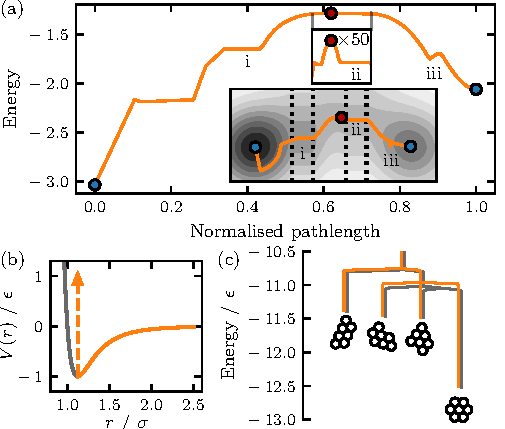
\includegraphics{flatdiscontinuous.pdf}
  \caption{\label{fig:bitss-flatdiscontinuous}
    Demonstration of BITSS applied to flat and discontinuous potentials.
    (a) Energy profile of the BITSS pathway on a 2D potential with flat regions.
        Blue and red dots denote the minima and transition state, respectively.
        Points of interest are labelled by i--iii (see text).
        Top inset: A zoomed in view around the transition state.
        Bottom inset: The pathway taken, with the edges of the flat regions marked by dashed lines.
    (b) The discontinuous hard-core pair potential used in the seven-particle cluster (orange).
        The standard Lennard-Jones potential is also shown in grey.
    (c) Disconnectivity graphs of the energy landscapes for the seven-particle cluster with the two potentials.
        The two graphs are offset for visibility.
  }
\end{figure}

The final challenges we will address are those related to complex landscapes that prove challenging for previous algorithms.
The first is the presence of flat regions in the landscape.
\Cref{fig:bitss-flatdiscontinuous}(a) shows BITSS applied to a 2D landscape with two such regions (i \& ii) that are flat in the $x$-direction.
We see BITSS is able to successfully converge past these flat regions, even with one very close to the transition state (ii).
In these regions there are no driving forces due to the potential and the energy constraint, which use purely local information about the gradient.
However, the distance constraint continues to pull the states together, preventing them from getting stuck.
When only a single state has a zero-gradient mode then the other is likely to slide down the potential slightly (iii), but the two states still remain either side of the dividing ridge and so the result is unaffected.

An additional consideration is the case where the potential energy surface is flat at the top of the pathway.
There are two possibilities here, one is that the potential is flat in a direction perpendicular to the tangent of the pathway, such that the ridge is level.
In this case BITSS is unaffected and it will be able to converge to some point along the ridge.
An example of this is the free global rotation and translation of the Lennard-Jones cluster in \cref{fig:bitss-testsystems}(a).
The other possibility is that the flat mode is in the direction of the pathway.
In this case there is no single transition state along the pathway, but instead a region.
BITSS would be ill suited in this situation because the equal-energy constraint would not prevent the images from passing over the saddle and falling to a minimum.

Finally, we investigate the application of BITSS to systems with undefined gradients, such as when the landscape is discontinuous.
To account for this, the equations for the coefficients must be adapted to not depend upon the gradients, and a gradient-free minimiser (simulated annealing) is used.
These changes are detailed in the methods section.
This has been tested using a 7-particle cluster with a hard-core Lennard-Jones pair-potential, shown in \cref{fig:bitss-flatdiscontinuous}(b), which results in a discontinuous landscape.
Using the gradient-free approach, BITSS is able to successfully find the transition states, allowing us to plot the disconnectivity graph of the system, shown in \cref{fig:bitss-flatdiscontinuous}(c).
Compared with the results for the standard Lennard-Jones cluster, the energies of the minima are largely unchanged, but the energies of the transition states are found to be slightly higher.
This indicates that the particles in the Lennard-Jones cluster cut the corner slightly as they transition, whereas this is not possible using the discontinuous potential, resulting in higher energies.
Despite this gradient-free method being feasible, it is worth noting that a gradient-based approach is significantly more efficient, and so should be preferred if possible.


\subsection{Multiple transition states}\label{sec:bitss-multits}
Here we test how the BITSS method performs when there are multiple transition states in the pathway between the two starting minima.
For this we use a 2D potential, shown in \cref{fig:bitss-multits}(a), with a pathway that follows two connected $135^\circ$ circular arcs.
The energy is given by the squared distance from this path, plus two Gaussian barriers resulting in transition states A and B, with energies $E_\text{A}$ and $E_\text{B}$.
We then vary $E_\text{B}$ between 0 and $E_\text{A}$, and the size of the distance reduction factor, $f$, to see if BITSS successfully converges to the higher transition state A.
For each pair of parameters we perform 5 runs with slight variations in the starting positions, with the results in \cref{fig:bitss-multits}(b) showing the points at which all 5 runs converge to the higher TS, A.

We see that if the difference between the two barriers is sufficiently large ($\gtrsim 10\%$) then BITSS always converges to the higher transition state.
However, as the difference decreases it starts to sometimes converge to the lower transition state if the separation is decreased quickly.
Therefore, to ensure that BITSS always converges to the higher energy transition state it may be necessary to restrict the separation step size.

Although the equal-energy constraint should cause the states to converge to A, this is not always the case because the discrete steps in the minimisation can cause the left image to jump over A before the other image passes B.
If the minimisation is fast and takes large steps then the chance for this to occur is increased.
Therefore, systems with complex, high-dimensional landscapes can probably successfully locate the highest transition state for larger values of $f$ and smaller height differences than simpler systems such as this 2D example.

\begin{figure}[htb]
  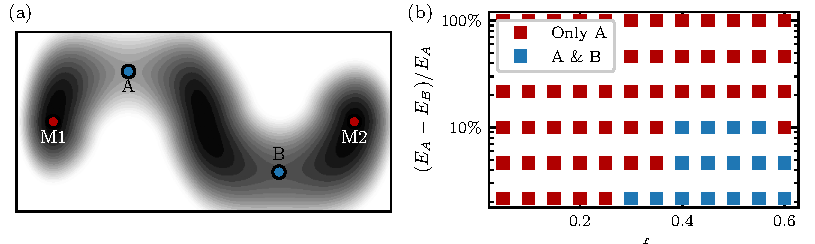
\includegraphics{multits.pdf}
  \caption{\label{fig:bitss-multits}
    (a) The potential used in the multiple TS test.
    M1 and M2 denote the two starting minima, and A and B are the two transition states.
    The energy of the barrier to B, $E_\text{B}$, is varied between 0 and $E_\text{A}$.
    (b) The results for the parameters under which BITSS reliably converges to A, and the points at which it sometimes converges to B.
    The x-axis is the BITSS distance reduction factor, $f$, and the y-axis is the relative difference between the two barrier heights.
  }
\end{figure}


\section{Conclusion}
Overall, we have developed the binary image transition state search (BITSS) algorithm for the efficient location of transition states in traditionally challenging landscapes.
This has distinct advantages for complex pathways owing to the lack of a required initial pathway estimate, as well as the identification of the transition state that provides the overall energy barrier in multi-step pathways.
From the speed analysis, we find that the combination of chain-of-states methods with single-ended transition state search methods provides good performance for near-linear pathways, such as for the Lennard-Jones cluster and cylindrical buckling.
However, for highly complex and non-linear pathways, as exhibited by the striped wetting example, BITSS is superior.
Indeed, the demonstrated speed and memory-efficiency will be key as we move towards studying larger and more complex systems using BITSS.

A second source of efficiency in the BITSS method comes from the ability to adaptively change the degrees of freedom as the algorithm proceeds.
We demonstrated how transition states could be found by both increasing the resolution upon convergence, and coupling systems with different discretisations.
The ease of coupling two copies of a system and adaptive remeshing, now leads to the possibility of incorporating BITSS into existing open-source optimisation methods, such as surface evolver \cite{Brakke1992} or finite element methods \cite{Kolev2021}, to provide important energy barrier functionality.

We also showed how BITSS can be used to survey discontinuous energy landscapes, demonstrated for a system of attractive hard-core particles.
This opens up possibilities for studying a broad range of systems previously out of reach of conventional landscape methods, but where transition information is valuable.
These include systems with very short range interactions, such as in colloidal clusters, or hard contact forces, such as in the folding of elastic materials, or locomotion and environmental interaction in robotics.

The distance metric between the two BITSS images is interesting to analyse further.
One question that emerges is whether transition states can be located by coupling two images through a small number of collective properties, rather than the total distance between all degrees of freedom in the system.
A second question concerns landscapes with multiple competing pathways between states.
In such cases, it may be possible to access transition states different from the most direct one by using a biased distance metric.
A further investigation that is now open to pursue is when discontinuities in the landscape occur at `stationary points' (now properly referred to as critical points).
In this case, a transition state can no longer be defined by its Hessian eigenvalues, but instead is more broadly defined as a region of locally minimal energy that separates two basins of attraction to minima.
Overall, it will be interesting to explore how BITSS enables access to even more challenging landscapes, and those not yet amenable to traditional landscape exploration techniques.

\begin{table}[]
  \begin{tabularx}{\textwidth}{>{\hsize=.5\hsize\linewidth=\hsize}C >{\hsize=.75\hsize\linewidth=\hsize}C >{\hsize=2\hsize\linewidth=\hsize}C >{\hsize=.75\hsize\linewidth=\hsize}C}
    \hline\hline
    Topic & Symbol & Parameter description & Value \\
    \hline
    \multirow{4}{*}{\rotatebox[origin=c]{90}{BITSS}}
            & $\alpha$ & Energy constraint strength & 10 \\
            & $\beta$  & Distance constraint error  & 0.1 \\
            & $f$      & Distance reduction factor  & 0.5 \\    
            & ---      & Coefficient recalculation regularity & 100 iterations \\    
    \hline
    \multirow{6}{*}{\rotatebox[origin=c]{90}{Buckling}}
            & ---            & Cylinder radius     & 50 \\
            & ---            & Cylinder length     & 80 \\
            & ---            & Mesh resolution     & 1.57 \\
            & ---            & Compressive strain  & 0.14\% \\
            & $k^\mathrm{S}$ & Stretching rigidity & 100 \\
            & $k^\mathrm{B}$ & Bending rigidity    & 1 \\
    \hline
    \multirow{8}{*}{\rotatebox[origin=c]{90}{Wetting}}
            & ---            & $x$ grid size                 & 200 \\
            & ---            & $y$ grid size                 & 200 \\
            & $\theta_a$     & Hydrophilic contact angle     & 60\si{\degree} \\
            & $\theta_b$     & Hydrophobic contact angle     & 110\si{\degree} \\
            & $\alpha_{12}$  & Interfacial width             & 1.77 \\
            & $\gamma_{12}$  & Surface tension               & 0.943 \\
            & $V_0$          & Droplet volume                & 4375 \\
            & $k_\mathrm{V}$ & Volume constraint coefficient & $10^4$ \\
    \hline
    \multirow{3}{*}{\rotatebox[origin=c]{90}{NEB}}
            & $k$ & NEB spring constant (LJ-7)     & 0.1 \\
            & $k$ & NEB spring constant (Buckling) & 0.01 \\
            & $k$ & NEB spring constant (Wetting)  & $10^{-6}$ \\
    \hline\hline
  \end{tabularx}
  \caption{\label{tab:bitss-params}
    Values of the parameters that are used throughout this chapter, unless otherwise specified.
    Some of the parameters for the buckling and wetting examples are described in the following chapter in \cref{sec:ell-potentials}.
  }
\end{table}

  \chapter{Energy Landscape Software Library}
\label{ch:software}
\graphicspath{{software/fig/}}
In this chapter, we discuss the aims and structure of the energy landscape library `ELLib', which has been developed in order to study large and versatile systems.
We detail the various potentials and methods that have been included in the library and how they have parallelised.
Finally, there is a demonstration of the library being applied to a structural optimisation problem.

The software library and the program used for the structural optimisation are both accessible in the supplementary materials, detailed in \cref{ch:appendix}.
Alternatively, the most up-to-date version of `ELLib' is available on GitHub at the link: \url{https://github.com/sjavis/ellib}.
This chapter provides details about how it can be used and will be further developed into comprehensive documentation in the near future.


\section{Software structure}
The energy landscape software is contained within an object-oriented C++ library that can be imported and run inside a user script or as a part of another program.
It has been designed in a modular manner so that different methods and applications can be easily interchanged and new methods can be implemented without difficulty.

At the core of almost all energy landscape methods is some form of energy minimisation, often with modifications, therefore ELLib contains a sub-library specifically for the minimisation methods.
Outside of this are the landscape exploration methods which make use of the minimisation, such as pathway and transition state search.
However, there is not always a clear division between the minimisation methods and the landscape methods.
For example, the genetic algorithm is a minimisation method but is not contained within the sub-library.
This distinction is made according to whether the method involves the minimisation of just a single state or multiple states, and whether further minimisation steps are involved within the method.

The minimisation sub-library is split into several core components.
Firstly, there is a class called \code{Potential}.
This provides the interface for calculating the energy and gradient for a given set of coordinates, and includes any potential specific parameters.
A \code{Potential} object can be created using functions for the energy and gradient, or using a predefined subclass.
The \code{State} class is used to create systems consisting of a potential and a set of coordinates.
These \code{State} objects are what the landscape and minimisation methods operate upon, and can be used to easily obtain the coordinates, energy, or gradient.
Each state can be parallelised onto multiple processors.
This uses a \code{Communicator} object that abstracts away the parallelisation using MPI, the details for which are given in \cref{sec:ell-parallel} below.
The final key component is the \code{Minimiser} class.
This provides the framework for the methods to minimise a single state.

A typical user script would likely use the energy minimisation methods in the following way:
\begin{itemize}
  \item Read in or initialise any required data.
  \item Create a \code{Potential} object using a predefined potential or make their own.
  \item Modify any potential parameters.
  \item Create a \code{State} object using the potential and some initial system coordinates.
  \item Create a \code{Minimiser} object, choosing the specific minimiser to use.
  \item Modify the minimisation parameters.
  \item Minimise the state.
  \item Final data analysis / output data.
\end{itemize}
A typical energy landscape user script may look like:
\begin{itemize}
  \item Set up data
  \item Create a \code{Potential} object and modify any parameters.
  \item Optionally, create a \code{Minimiser} object.
  \item Initialise a landscape method with the potential and minimiser and choose parameters.
  \item Run the landscape method.
  \item Final data analysis / output data.
\end{itemize}
Users may also combine multiple methods into a single script or use them as part of a larger program.


\section{Parallelisation}\label{sec:ell-parallel}
A primary aim of the software is to be able to utilise computational clusters for high performance computing in order to speed up large-scale systems.
Therefore, the code is designed to be parallelised using MPI (message passing interface), which distributes the memory across the computational processors and uses messages to pass necessary data among them.
This has been implemented in such a way as to abstract away the details of the parallelisation.
This enables users who are either developing new methods and potentials or primarily interested in applications to make use of the parallelisation with minimal effort or knowledge of MPI.

The parallelisation is performed on each \code{State} object.
By default each state is split among all of the processors, but specific processors may also be assigned to a given state when it is created.
The state's coordinates are split into blocks, one for each processor, which are then stored in a vector locally.
Any coordinates that the processor requires for computing the energy and gradient of its block are then stored at the end of this vector (the halo coordinates).
The updating of these halo regions and all other communication between the processors is handled by an internal \code{Communicator} object.
\code{State} offers functions to either calculate the energy and gradient contributions specific to each processor's block (\code{blockEnergy} and \code{blockGradient}), or the total energy and gradient (\code{energy} and \code{gradient}) which uses MPI communication in the background.
Likewise, the \code{blockCoords} functions can be used to read and assign the local coordinate vector, and \code{coords} can be used to read and assign the whole system coordinates.

In order for a specific potential to make use of the software's parallel framework it must be defined in such a way that the halo coordinates can be determined automatically.
To do this, the calculation of the energy and gradient are split into separate elements that each rely only upon a small number of degrees of freedom.
These elements also include a label for the type and any parameters specific to that element.
The potential must then have an \code{elementEnergyGradient} function defined that will compute the contributions to the energy and gradient for each individual element.
For some potentials it may not be possible to split it neatly into separate elements.
If this is the case, then there is a backup \code{blockEnergyGradient} potential that can be defined.
The state's \code{Communicator} object is passed to this function, which can be used to manually communicate between the processors.

The \code{Communicator} object itself is initialised automatically when a State is created.
This will first split the system coordinates into the blocks for each processor.
Currently there is no attempt to optimise this, it requires that the user define the coordinates in a logical order so that the halo regions are kept small.
There is potential scope to improve this in the future so that the order of coordinates is changed to reduce the halo regions.
Next, each element is assigned to a processor based upon which block contains the most of its degrees of freedom.
Any of this element's coordinates that are contained on other blocks are therefore in the halo region.
Once this is done, new MPI data types are created that will send the required data to update the halos of the other processors.
In order to use this, a \code{communicate} function is defined which will update the halo of whatever vector is passed to it, typically, the coordinates or gradient vector.
The \code{Communicator} also has several other useful functions, such as \code{assignBlock} and \code{assignProc}, which take a vector with the total number of degrees of freedom and return a vector of the local block, or the block and the halo, respectively.
Furthermore, there are additional functions included, such as \code{sum} and \code{dotProduct}, that first perform operations on vectors locally before summing the result across the processors used in this Communicator object.



\section{Potentials}\label{sec:ell-potentials}
An underlying system potential is necessary in order to study an energy landscape.
In the software library, these can be created using the \code{Potential} class or a subclass.
This potential can be defined by the user by providing \code{energy} and \code{gradient} functions, or a single function to compute both, \code{energyGradient}.
If instead, it is to be run in parallel then the \code{elementEnergyGradient} and \code{blockEnergyGradient} functions should be used, as described in the previous section.
If the potential also needs to set up parameters, then there is an \code{init} function, which is called when the potential is used to create \code{State} object.

The user may also make use one of several predefined potentials: \code{Lj2d}, \code{Lj3d}, \code{BarAndHinge}, \code{PFWetting}. Each of these potentials is described below.


\subsection{Lennard-Jones}
A Lennard-Jones particulate model has been implemented for both 2D and 3D, which can be accessed using \code{Lj2d} and \code{Lj3d}.
For a set of particles with positions ${\bm{x}_1, \ldots, \bm{x}_N}$ the model gives an energy of
\begin{equation}
  E(\bm{x}_i) = \sum_{i, j \ne i} 4 \epsilon \left[ \left(\frac{\sigma}{r_{ij}}\right)^{12} - \left(\frac{\sigma}{r_{ij}}\right)^{6} \right] \quad \text{where} \quad r_{ij} = \sqrt{\sum_k (x_{i,k} - x_{j,k})^2}.
  \label{eq:ell-lj}
\end{equation}
The parameters $\epsilon$ and $\sigma$ are the inter-particle potential well depth and the particle size, respectively.
These can be set in the code using the \code{epsilon} and \code{sigma} parameters, each beginning with a value of one.
The gradient of the energy with respect to each degree of freedom is then given by,
\begin{equation}
  \frac{\partial E}{\partial x_{i,k}} = 24 \epsilon \sum_{j \ne i} (x_{i,k} - x_{j,k}) \left( \frac{\sigma^{6}}{r_{ij}^{8}} - \frac{2\sigma^{12}}{r_{ij}^{14}} \right).
\end{equation}

At present this potential cannot be run in parallel, as Lennard-Jones systems are not the focus of this PhD work.
In future parallelisation could be implemented in order to study large clusters with short range interactions.
However, this would require the particles to be redistributed among the processors according to their location, which is beyond the current limits of the software.


\subsection{Bar and Hinge Triangulated Surface Model}\label{sec:ell-bah}
The software contains a bar-and-hinge model to simulate thin elastic surfaces (\code{Bar\-And\-Hinge}).
This represents the surface as a triangular mesh, within which, each bond is an elastic spring, and each pair of adjacent triangles is connected by an elastic hinge.
The total elastic energy is, therefore,
\begin{equation}
  E = \sum_i \frac{k^\text{S}_i}{2} (r_i - r_{0i})^2 + \sum_j \frac{k^\text{B}_j}{2} (\theta_j - \theta_{0j})^2,
\end{equation}
where the first sum gives the stretching energy due to each bond $i$, with length $r_i$, equilibrium length $r_{0i}$, and stretching rigidity $k^\text{S}_i$.
The second sum provides the bending energy, where $\theta_j$ is the dihedral angle, $\theta_{0j}$ is the equilibrium angle, and $k^\text{B}_j$ is the bending rigidity of hinge $j$.
In the software $k^\text{S}$ and $k^\text{B}$ values can be set using the \code{setRigidity} function.
It is also possible to set the equilibrium lengths and angles, but otherwise they will be calculated from the initial configuration of the mesh.
The triangulation itself is applied using \code{setTriangulation}.
This takes a list of the three node indices for each triangle.
These must all be listed in the same order, either clockwise or anticlockwise, to ensure that the surface is properly oriented and so that the dihedral angles can be evaluated across the full $2\pi$ range.

\begin{figure}[htb]
  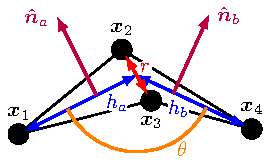
\includegraphics{BAHschematic.pdf}
  \caption{\label{fig:ell-BAHschematic}
    Schematic of the bar and hinge model showing the relevant parameters for a single hinge element.
    $h_i$ and $\bm{\hat{n}}_i$ denote the height and unit normal of each triangle respectively.
  }
\end{figure}

The expressions for the gradient of the energy can be obtained by considering the stretching and bending energies of an individual bond and hinge.
For simplicity, the indices for the bond and hinge are ignored.
Using the variables shown in the schematic in \cref{fig:ell-BAHschematic}, the gradient of the stretching energy of the bond between $\bm{x}_2$ and $\bm{x}_3$ is given by
\begin{equation}
  \frac{\partial E^\text{S}}{\partial \bm{x}_2} = - \frac{\partial E^\text{S}}{\partial \bm{x}_3} = k^\text{S} (r - r_0) (\bm{x_2} - \bm{x_3}).
\end{equation}
The gradients of the bending energy of the hinge are
\begin{align}
  \frac{\partial E^\text{B}}{\partial \bm{x}_1} &= k^\text{B} (\theta - \theta_0) \frac{\bm{\hat{n}}_a}{h_a}, \\
  \frac{\partial E^\text{B}}{\partial \bm{x}_2} &= - k^\text{B} (\theta - \theta_0) \left[\frac{\bm{\hat{n}}_a}{h_a} + \frac{\bm{\hat{n}}_a + \bm{\hat{n}}_b}{r}\right],
\end{align}
\begin{align}
  \frac{\partial E^\text{B}}{\partial \bm{x}_3} &= - k^\text{B} (\theta - \theta_0) \left[\frac{\bm{\hat{n}}_b}{h_b} + \frac{\bm{\hat{n}}_a + \bm{\hat{n}}_b}{r}\right], \\
  \frac{\partial E^\text{B}}{\partial \bm{x}_4} &= k^\text{B} (\theta - \theta_0) \frac{\bm{\hat{n}}_b}{h_b}.
\end{align}

These models have been widely applied to study origami structures \cite{Liu2017a,Gillman2018,Zhou2023}, where the triangular mesh is made to match the geometry of the crease pattern.
Alternatively, it can also be used to model continuous elastic surfaces by choosing the spring constants in such a way that they accurately represent the elastic moduli in the continuum limit.
In which case, the spring coefficients are given by \cite{Gelder1998,Seung1988,Grinspun2006},
\begin{gather}
  k_\text{S} = Yt \cdot \frac{A_\text{sum}}{r_0^2}, \\
  k_\text{B} = \frac{Yt^3}{12(1-\nu^2)} \cdot \frac{r_0^2}{A_\text{sum}},
\end{gather}
where $Y$ is the Young's modulus, $t$ is the thickness of the surface, and $\nu$ is the Poisson's ratio.
The value $A_\text{sum}$ is the total area of the adjacent triangles at equilibrium, of which there will be one for bonds on the boundary, and two for the others.
This method is used if the rigidities have not been directly set, and the \code{thickness} parameter is provided.
This can take a different value for each node of the mesh in order to create a varying thickness.
In this case an average is taken for each bond and hinge.

This model is particularly useful for its simplicity and speed, however it has some limitations on its accuracy compared to real structures.
Firstly, because it is a 2D surface, the thickness is assumed to be much smaller than the dimensions along the surface itself.
This is particularly important since the one-dimensional folding of adjacent triangles cannot accurately model the effect of twisting, but this will be negligible as long as the thickness is sufficiently small.
This is because any twisting of a thin surface requires some in-plane stretching, the energy of which scales proportionally to the thickness, $t$, while twisting energy scales as $t^3$.
Similarly, it cannot model the energy due to Gaussian curvature, the product of the two principal curvatures.
However, the high resistance to stretching makes this negligible in most circumstances, and, if the boundary is fixed or the surface is closed, the total energy due to the Gaussian curvature is topologically constant according to the Gauss-Bonnet theorem \cite{Rueda-Contreras2021}, so it may be safely ignored.
Finally, another limitation of the model is that the Poisson ratio under stretching cannot freely be tuned.
Instead, it depends upon the geometry of the mesh.
For example, if an equilateral triangular mesh is used then the Poisson ratio will be 1/3, regardless of the spring constants that are applied \cite{Gelder1998}.
These limitations mean that the model is primarily of use to study elasticity problems where bending is the dominant effect.

An additional energy contribution is possible by incorporating an external force with the \code{force} parameter.
This can be a uniform force to model gravity, or a magnetic field; or applied inhomogeneously across the structure such as to initialise random structures.
It is also possible to include interactions with a substrate using \code{setWall}, which turns on a Lennard-Jones 3-9 potential, which is obtained by considering an interaction between a particle and an infinite wall of particles that interact by the standard Lennard-Jones potential, \cref{eq:ell-lj}.
\begin{equation}
  E(h) = \epsilon \left( \frac{2}{15}\left(\frac{\sigma}{h-h_0}\right)^9 - \left(\frac{\sigma}{h-h_0}\right)^3 \right),
\end{equation}
where the height above the wall, $h$, has been shifted by $h_0$ to ensure that the energy is minimal at $h=0$.
The Lennard-Jones parameters $\sigma$ and $\epsilon$ are initially set to $10^{-12}$ and $10^{-5}$, which tend to give results that correspond to levels of adhesion observed in experiments.
But the precise adhesion energy, controlled by $\epsilon$, will depend upon system size and so should be adjusted for different applications.
The adhesion arises because the potential is attractive for $h>0$, but if this is not desired, it can be switched of, in which case the potential is cut off at $h=0$ and shifted so that $E(0)=0$.

This potential uses the software's parallel framework by splitting the contributions to the energy into energy elements.
The stretching energy uses one element for each pair of particles, and the bending energy has one element for the four particles in pair of triangles.
If the force and substrate interactions are switched on, they each have one element per particle.


\subsection{Phase Field Model}
In order to model multicomponent fluid systems a phase field model has been implemented, \code{PFWetting}.
This potential has been implemented with two variants: a binary fluid and an $N$-fluid version, which can be accessed by modifying the \code{nFluid} parameter.
This method uses a square grid (resolution size $\delta$) where each node is marked as either solid or a fluid using \code{setSolid}.
If a fluid node is adjacent to a solid node then the solid surface passes through the center of the node, and the volume $V$ and surface area $A$ take different values from the bulk.
Each fluid has a concentration, $C_i$, for each fluid $i$ (for the $N$-fluid variant) or an order parameter, $\phi = C_1 - C_2$ for the binary model.
These concentrations take bulk values of 0 or 1 depending on if the fluid is located at that position, and smoothly vary, resulting in diffuse fluid interfaces.

This potential has four or five contributions to the overall energy depending upon whether it is using the binary or $N$-fluid model.
One sets the bulk fluid values, $E^\text{B}$, and another includes the interfacial energy of the fluids, $E^\text{I}$.
If the $N$-fluid model is used, there is also a soft energy constraint to ensure that the total concentration is the same everywhere, $E^\text{D}$.
Next, there is a fluid-solid interaction, $E^\text{S}$.
Then, finally, there is either an energy penalty to set a constant volume across the system, $E^\text{V}$, or the energy due to the pressure of the system, $E^\text{P}$.

The $E^\text{B}$, $E^\text{I}$, and $E^\text{D}$ terms each apply to the whole of the fluid domain.
Therefore, they are split into single elements for each fluid node in the system so that the potential can be computed in parallel.
The energies of these discrete elements are then given by,
\begin{equation}
  E^\text{B} =
  \begin{cases}
    \frac{\kappa}{16} (\phi + 1)^2 (\phi - 1)^2 V & \text{binary},\\
    \sum_{i=1}^{N} \frac{\kappa_i}{2} C_i^2 (C_i - 1)^2 V & \text{$N$-fluid},
  \end{cases}
  \label{eq:ell-PFEB}
\end{equation}
\begin{equation}
  E^\text{I} =
  \begin{cases}
    \frac{\kappa'}{4} (\grad \phi)^2 V & \text{binary},\\
    \sum_{i=1}^{N} \frac{\kappa'_i}{2} (\grad C_i)^2 V & \text{$N$-fluid},
  \end{cases}
  \label{eq:ell-PFEI}
\end{equation}
\begin{equation}
  E^\text{D} =
  \begin{cases}
    0 & \text{binary},\\
    k^\text{V} \left( 1 - \sum_{i=1}^{N} C_i \right)^2 V & \text{$N$-fluid}.
  \end{cases}
  \label{eq:ell-PFED}
\end{equation}
\Cref{eq:ell-PFEB} uses a double well potential to ensure that the energy is minimised when the fluid concentrations are 0 or 1.
\Cref{eq:ell-PFEI} penalises any fluid interfaces where the gradient of the concentrations / order parameters are non-zero.
\Cref{eq:ell-PFED} ensures that the sum of the concentrations is equal to one by using a large constraint coefficient $k^\text{V}$.
The parameters $\kappa_i$ and $\kappa'_i$ are related to the interfacial tensions, $\gamma_{ij}$, and widths, $\alpha_{ij}$.
This can be determined by finding the fluid concentration function that minimises the energy given by the continuous analogue of \cref{eq:ell-PFEB,eq:ell-PFEI}, giving the following relations,
\begin{gather}
  \gamma_{ij} = \frac{\sqrt{\kappa_i+\kappa_j} \sqrt{\kappa'_i+\kappa'_j}}{6},\\
  \alpha_{ij} = \sqrt{\frac{\kappa'_i+\kappa'_j}{\kappa_i+\kappa_j}}.
\end{gather}
They are assigned by the \code{setSurfaceTension} and \code{set\-Interface\-Width} functions, and used to calculate $\kappa_i$ and $\kappa'_i$.
However, if four or more fluids are used, the full set of surface tensions cannot be matched because there are not enough parameters in the model.
Alternative models that allow all surface tensions to be prescribed are available in the literature, such as \cite{Dong2018}.

Each of these energy elements includes the neighbouring nodes in order to calculate the gradients in \cref{eq:ell-PFEI}.
Generally these use central difference, however forward difference is used if one side is a solid node.
For example, the $x$-gradient of $\phi$ at a point where $x=x_0$ is
\begin{equation}
  \frac{\partial \phi}{\partial x} =
  \begin{cases}
    \frac{\phi(x_0+\delta) - \phi(x_0-\delta)} {2\delta} & \text{for bulk fluid},\\
    \frac{\phi(x_0+\delta) - \phi(x_0)} {\delta}         & \text{if solid at $x_0-\delta$},\\
    \frac{\phi(x_0) - \phi(x_0-\delta)} {\delta}         & \text{if solid at $x_0+\delta$}.\\
  \end{cases}
\end{equation}
The equations for the energy gradients at each element are therefore given by
\begin{align}
  \frac{\partial E^\text{B}}{\partial \phi} = \frac{\kappa}{4} \phi (\phi^2 - 1) V \qquad& \text{binary},\\
  \frac{\partial E^\text{B}}{\partial C_i} = \sum_{i=1}^{N} \frac{\kappa_i}{2} (2C_i^3 - 3C_i^2 + C_i) V \qquad& \text{$N$-fluid}.
\end{align}

The interaction between the fluid and solid is designed to apply partial wetting behaviour, such that the fluid interface meets the solid surface at a specific contact angle, $\theta$.
This contact angle can be defined by a function across the domain using \code{setContactAngle}.
The interaction uses a cubic wetting potential, where the gradient is zero at the bulk fluid concentrations in order to avoid enrichment of the fluid concentration at the surface.
This energy relies only upon the local fluid values at the surface, so the energy is split into one element per surface node with
\begin{equation}
  E^\text{S} = \frac{1}{\sqrt{2}} \cos{\theta} \left( \frac{\phi^3}{3} - \phi - \frac{2}{3} \right) A.
\end{equation}

Finally the pressure and volume energies are given by,
\begin{gather}
  E^\text{P} = p V_\text{tot},\\
  E^\text{V} = k_\text{V} (V_\text{tot} - V_0)^2,
\end{gather}
where $p$ and $V_0$ are the chosen pressure and volume, and $V_\text{tot}$ is the total volume of the fluid.
Unlike the energy contributions, the calculation of $V_\text{tot}$ relies upon the whole system, so it cannot be assigned to separate energy elements and requires special treatment using the \code{blockEnergyGradient} function.
Therefore, the fluid volume is first calculated on each block and then added up across the processors, reducing the overhead required for MPI.



\section{Implementation of minimisation methods}
The \code{Minimiser} class contains the framework for optimising a single state to a (usually local) minimum in the energy landscape.
Therefore, it does not encompass ensemble minimisation methods, such as Genetic Algorithm, which will be discussed in the next section.
The methods that have been implemented are:
\begin{itemize}
  \item Gradient descent (\code{GradDescent})
  \item L-BFGS (\code{Lbfgs})
  \item FIRE (\code{Fire})
  \item Simulated annealing (\code{Anneal})
\end{itemize}


These methods are themselves subclasses of \code{Minimiser} and implement functions that are called during a minimisation.
The first is an \code{init} function that can be used if any set up is required at the start, including the instantiation of parameters.
Then the main loop is run, during which the \code{iteration} function is called which contains the main part of the methods.
At the end of each iteration a \code{checkConvergence} function detects if it has reached the minimum, at which point the method ends.
A user defined function may also be passed into the minimisation that is called at the start of each iteration to modify system parameters.
This provides flexibility to the user and could be used, for instance, to steadily perturb the system during the start of the minimisation, or to save the trajectory of the minimisation.

\code{Minimiser} also has parameters generic to most or all of its subclasses.
Namely, the maximum number of iterations and which line search method should be used, if at all.
Currently, backtracking line search is included, which ensures that the energy decreases sufficiently to satisfy the Armijo rule, \cref{eq:lm-ls-armijo}, with $c_1=0.5$, or optionally, that the energy never increases more than a chosen amount.

\subsection{Gradient descent}
The gradient descent implementation has one additional parameter \code{alpha}, which is the step size factor, $\alpha_i$, in \cref{eq:lm-graddescent}.
This has a default value of $0.1$, although the actual step size will be determined using a line search.
So, unless it is turned off, the value of \code{alpha} is not hugely important.
In order to check for convergence, the root mean square of the gradient, $\abs{\grad E} / \sqrt{N}$, where $N$ is the number of degrees of freedom, is compared to the \code{convergence} parameter that is chosen for the \code{State} object.
This same criterion is also used for both L-BFGS and FIRE.

The gradient descent algorithm is also very amenable to parallelisation by distributing the degrees of freedom between processors.
This is because communication between the processors are only required at three points: to communicate the gradient to the halo nodes, computing the magnitude of the gradient for the root mean square, and calculating the energy for the line search.
The latter may require multiple communications, depending upon the number of iterations, but if no line search is used then just the two communications are necessary.

\subsection{L-BFGS}
As for the implementation of L-BFGS, there are two additional parameters.
The first is the number of steps to store to calculate the search direction, $m$, which has a default value of five.
Secondly, \code{maxStep} can be used to restrict the step size in each iteration, such that, if the step is greater than this, it is rescaled to the maximum value.
This can be useful, for example, to ensure that the minimisation is smooth when the trajectory is used to approximate an MEP.
If this value is not manually set, then no restriction is made.

Currently, if L-BFGS is run in parallel, then only the calculations of the gradient and line search are split among the processors, while the calculation of the search direction is instead performed in serial.
This is because $2m+2$ dot products are required when calculating \cref{eq:lm-lbfgs-q0,eq:lm-lbfgs-q,eq:lm-lbfgs-z0,eq:lm-lbfgs-z}, and each would require a separate communication.
Therefore, the search direction is calculated in serial by collecting the whole of the gradient on each processor in an attempt to reduce the number of MPI communications.

\subsection{FIRE}
The \code{Fire} object has a parameter \code{dtMax}, which is the maximum timestep that is allowed when updating the velocity and the position.
Ideally, an appropriate value should be assigned by the user.
However, if none are provided, then a reasonable value will be estimated using the energy gradient at the start of the initialisation,
\begin{equation}
  \Delta t_\text{max} = \frac{1}{10 \sqrt{\abs{\grad E}}}.
\end{equation}
This will result in a step size that is independent of the scale of the energy, so, if the gradients are very high it will not cause very large step sizes.
The step size would instead be on the order of $0.1$, which may not be accurate for particularly large or small system sizes.
In the unusual circumstance that the gradient is initially zero, \code{dtMax} is simply set to one.
Since FIRE is an inertial optimisation method that uses a continually updated velocity, the line search is off by default.
However, it can be switched on, in which case the importance of the timestep is reduced.

In contrast to L-BFGS, FIRE does not require so many communications between processor nodes, and so is efficient for parallelisation.
Aside from communicating to update the halo nodes, the only other communication that is required is to calculate the magnitudes of the gradient and the velocity, and their dot product.
Therefore the method never requires collecting all degrees of freedom on a single processor.

\subsection{Simulated Annealing}
To use simulated annealing an \code{Anneal} object can be created using two parameters: \code{displacement} and \code{tempInit}.
Suitable values for these cannot be easily guessed, so the user is required to provide them.
The former is used in calculating the random trial state for each iteration.
For each degree of freedom a perturbation is picked from a uniform distribution where the maximum value is given by \code{displacement}.
The second parameter \code{tempInit} describes the initial temperature, which should be high enough to allow the system to adequately explore the energy landscape.
The precise function describing how the temperature decreases over time may be set by the user using the \code{coolingSchedule} parameter, but the default function uses linear multiplicative cooling \cite{Junn2017}, such that, at iteration $i$, the temperature is
\begin{equation}
  T(i) = \frac{T_0}{1 + ki},
\end{equation}
where $T_0$ is the initial temperature, and $k$ is the cooling rate, which can be adjusted via the parameter \code{coolingRate} which has a default value of 1.

Because simulated annealing is not a gradient-based minimiser and it is attempting to find the global minimum rather than local minima, convergence should not be determined using the root mean square of the gradient.
Instead, the state is determined to be converged once the trial state has been rejected more than a certain number of iterations in a row, which is given by the \code{maxRejections} parameter.
This is initially set to zero, in which case the method is allowed to continue until it reaches the maximum number of iterations.

Simulated annealing is performed almost completely in parallel.
The only communications required are to sum up the total energy of the state, to communicate the random perturbations to the halo coordinates, and to share the same random test value so that all processors agree on whether to accept or reject the step.



\section{Implementation of energy landscape methods}
The main ELLib library contains the more general energy landscape methods that typically make use of the minimisation algorithms in order to find transition states, pathways, and in the search for minima.
Because they cover a variety of methods, they do not follow any rigid structure, unlike the minimisation methods.
Each method is implemented in a class which can be used by creating an object for the method, modifying any parameters, and then calling a \code{run} function.
This function outputs the result for the method, whether that be a global minimum configuration, transition state, or pathway.
Each class may also have functions for obtaining other information from the method.

The currently implemented methods are the genetic algorithm for finding global minima, the BITSS method for locating transition states, and NEB to find pathways.
In the future we hope to expand this to include other methods, such as basin hopping, eigenvector-following, and the string method.


\subsection{Genetic Algorithm}
The genetic algorithm is implemented in the \code{GenAlg} class.
This takes a \code{Potential} object that is be used to generate a population of states.
The size of this population is given by \code{popSize}, and the total number of generations, \code{maxIter}.
Each of these are initially set to 100.

There are two possibilities for initialising the population.
Firstly, a function may be provided by the user to individually generate states (assiged using \code{stateGen}).
Alternatively, \code{bounds} can be set to the upper and lower bounds for each degree of freedom.
The coordinates for the states are then randomly generated between these bounds.
If neither of these are set then there is no way of determining suitable coordinates for the states, so the method will not run.

In order to create a new generation, the parents can be selected using one of two methods, either roulette selection (the default), or simply choosing the most fit.
This is set by the \code{selectionMethod} parameter, with the number of parents chosen as fraction of the population according to \code{selectionRate}.
Elitist selection is also possible by setting \code{numElites} to be the number of the best states that should be passed directly to the next generation.
The remaining children are then created using uniform crossover between pairs of parents.
Each of the child's coordinates may then be mutated with a probability given by \code{mutationRate}.
This mutation is chosen from a uniform distribution with a standard deviation chosen by the \code{perturbation} parameter.
If this is not set, but the bounds are, then the standard deviation is 1\% of the total allowed range.

The genetic algorithm implementation also has a couple of other useful features.
Firstly, it can also be run as a Lamarckian hybrid approach by passing a \code{Minimiser} object to use for the local search.
This allows it to more quickly identify and explore local minima in the landscape.
Secondly, a generic user-defined function can be called in each generation to access and modify the population.
This can be used, for example, to output the fittest state from each generation.

The standard behaviour is to continue until the full number of generations has been reached, but there are two possible methods for stopping early if it is deemed to have converged.
The first is a user-defined energy limit, such that if a state is found with a lower energy it will stop.
This could be useful if the precise global minimum is not needed and all that is desired is a low energy solution.
The second method halts the method if it has gone a certain number of generations without seeing any improvement in the fittest individual.
These two methods and their criteria can be applied using the \code{setConvergence} function.

The method by which the genetic algorithm is parallelised depends on the number of processors relative to the size of the population.
If the population size is greater than or equal to the number of processors then each state is run on just a single processor.
This is particularly efficient because the processors only need to communicate when setting each new generation, while the energy of each state is computed in serial.
On the other hand, if there are more processors, then each state is distributed among two or more processors.
This may be useful if the potential is particularly complex or a hybrid method is being used.
This parallelisation is most efficient when the population size is a multiple / factor of the number of processors.
Otherwise, some processors will be assigned a larger share of the work, and the others will spend time idle.

\subsection{BITSS}
The \code{Bitss} class provides the implementation of the BITSS method, and is initialised using two states and a minimiser.
These two states provide the initial coordinates for the method, so they are typically selected to be the minima.
The \code{Bitss} class creates a new \code{State} object and an associated \code{BitssPotential}.
These wrap around the two individual states in order to calculate the full energy of the pair of states, including the constraints.

The most significant parameter for BITSS is the fraction to reduce the distance for each iteration.
This is given by \code{distStep} with a value of 0.5, but this may be too rapid for some applications, and should be changed accordingly.
Typically, the method should run until convergence or failure, but \code{maxIter} can be set to halt the method after a large number of iterations, with an initial value of 100.
If \code{distStep} is reduced significantly then this will likely need to be increased.
To calculate the separation between the states the Euclidean distance is often used, but the user is free to use any metric.
This can be done by passing functions for the distance and its gradient to the \code{distFunc} parameter.

The constraint coefficients are recalculated throughout each minimisation according to the \code{coefIter} parameter, which is initially every 100 iterations.
During this recalculation the energy barrier is estimated using a linear interpolation, but for some applications this may be many orders of magnitude too large when the states are far from TS.
To prevent this from causing an issue, the \code{maxBarrier} parameter may be set to a reasonable value.
It is also possible to alter the $\alpha$ and $\beta$ parameters from \cref{eq:bitss-ke,eq:bitss-kd}, using \code{alpha} and \code{beta}, but they can usually be left at their recommended values of 10 and 0.1, respectively.
To prevent issues associated with recalculating the coefficients, it is recommended to switch off the line search for the minimisation.
Furthermore, if no minimiser is provided then it defaults to L-BFGS with the line search automatically switched off.

The convergence to the TS can be based on one of five methods.
Two of these are based upon the separation constraint reaching a chosen size, whether that be the actual distance, or the distance relative to the initial separation.
The next criteria are based upon the estimate of the TS.
The third criterion relates to the root mean square of the gradient at the estimate, while the fourth uses the change of the estimate from one iteration to the next.
Finally, the uncertainty of the TS energy can be used.
This is calculated as the difference between the energy of the TS estimate, $E_\text{TS}$, and the pair of states, $E_i$, relative to its height above the initial state energies, $E_{i,0}$,
\begin{equation}
  \epsilon_E = \frac {E_\text{TS} - \langle E_1, E_2 \rangle} {E_\text{TS} - \langle E_{1,0}, E_{2,0} \rangle},
\end{equation}
where $\langle\cdots\rangle$ denotes the average.
Each of these methods can be set using the \code{set\-Convergence\-Method} function, which is initially set to a relative distance criteria of 1\%.

The coordinates of the TS are output by the \code{run}, but other information can also be extracted.
The final two states can be obtained using the \code{getPair} and \code{getPairCoords} functions, which return two \code{State} objects or vectors, respectively.
Meanwhile, the \code{getTS} and \code{getTSCoords} functions give the state and coordinates of the TS estimate midway between the pair.
\code{Bitss} can also report if it believes it has not successfully found the TS if the \code{getFailed} function is called.
This is based upon any of three conditions: if the final state did not properly converge, if $\langle E_1, E_2 \rangle < \max(E_{1,0}, E_{2,0})$, or if $E_\text{TS} < \langle E_1, E_2 \rangle$.

The BITSS method can be run in parallel to distribute the calculation of the energies and gradients of the individual states, but the energy contributions of the constraints are computed in serial.
This is because the total energy needs to be known for the energy constraint, and the full set of coordinates are needed to calculate the separation between the two states.
However, the effect of this is relatively minor because the calculation of the underlying potential tends to be much more costly.

% \subsection{Climbing Image}

\subsection{Nudged elastic band (NEB)}
The \code{Neb} class encompasses several variations of the NEB method, including a hybrid climbing image method and DNEB.
The latter of which may also be accessed using the \code{Dneb} wrapper class.
There are two ways that the method may be initialised, either using a set of coordinates for the initial chain, or by passing the end points and the number of states (including the end points), in which case the chain is set by a linear interpolation.

Similar to BITSS, the NEB implementation uses a single \code{State} object with \code{NebPotential} which calculates the total energy of the elastic band.
This delegates the computation of the single state energies to a set of \code{State} objects for each image along the chain.
This main \code{State} is then minimised to find the pathway.
Because NEB and DNEB modify the gradient of the energy, the minimisation should, again, not use a line search, and the default L-BFGS minimiser has it switched off by default.

The elastic spring constant, $k$ in \cref{eq:lm-neb-energy}, can be set using the \code{kSpring} parameter, which is initially set to one.
This should not be too large or too small because it may cause the potential or equal spacing constraint to be washed out and the method may take longer to converge.
The tangent vectors used to project the components of the forces are obtained using the bisection method, described by \cref{eq:lm-neb-taubisect}.

To utilise a hybrid climbing image method the \code{setHybrid} function may be called.
This is also used to set the \code{hybridIter} variable, which activates the climbing image at a chosen iteration, allowing the the chain to first approximate the pathway.
After this, at each iteration, the state with the highest energy is selected and its driving force is replaced by the climbing image force, \cref{eq:lm-ci-force}.

The \code{run} function performs the initialisation and optimisation of the chain and outputs the coordinates along the pathway.
Subsequent outputs can be acquired using \code{getChain}, \code{getCoords}, and \code{getEnergies}.
These methods provide the final list of \code{State} objects, the list of coordinates, and the list of energies, respectively.

The method allows the chain of states to be distributed among the available processors so that the calculations of the single state energies and gradient are performed in parallel.
These are either allocated with multiple states per processor or multiple processors per state, using the same approach as the genetic algorithm.
The results from the individual states are then broadcast to all processors so that the total energy and gradient can be computed serially.
Although the full energy and gradient could possibly be calculated in parallel, this would significantly complicate the method, and much like BITSS, the main computational cost is usually associated with the single state energy calculations.

% \subsection{Benchmarking}
% \subsubsection{Minimisation}
% \subsubsection{Transition state search}

% \subsection{Parallelisation}
% In order to study how the methods scale under parallelisation, 2D wetting simulations are performed using the \code{PFWetting} potential and their runtimes are recorded.
% A $90\times90$ system size is used for this with a solid surface at the bottom, which has alternating hydrophilic and hydrophobic regions with contact angles of $60^\circ$ and $120^\circ$, respectively.
% The total volume of the liquid is constrained to that of a semi-circular drop with radius of 30 in lattice units, which is used to initialise the minimisation tests.
% The various system parameters are: \code{interfaceSize}$=1$, \code{surfaceTension}$=1$, \code{volConst}$=10^4$, and a root-mean-square gradient convergence criteria of $10^{-4}$.
% The minima and transition state for this system are shown in \cref{fig:ell-parallel}(a).

% \begin{figure}[htb]
%   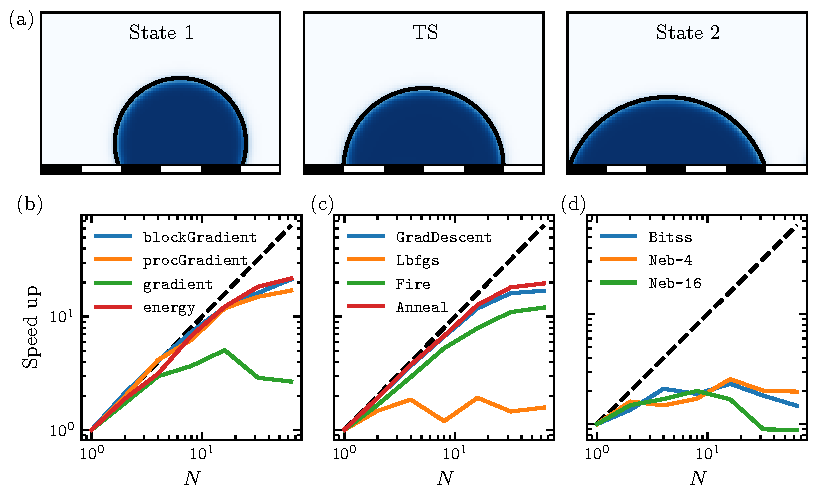
\includegraphics{parallel.pdf}
%   \caption{\label{fig:ell-parallel}
%     (a) The stable states and transition state for the parallelisation test system.
%         The top third of the simulation height has been removed.
%         Black regions indicate hydrophilic sections of the solid, and the white regions are hydrophobic.
%     (b-d) Comparison showing how much the runtime is reduced with different numbers of processors, $N$, compared to a single processor for each method.
%           The dashed line shows the optimal speed up (equal to the number of processors).
%     (b) Energy and gradient calculation methods.
%     (c) Minimisation methods.
%     (d) Energy landscape methods.
%   }
% \end{figure}

% First, various energy and gradient functions are tested by randomly altering the local coordinates and then computing the function \num{100000} times.
% These each perform different types of MPI communication, so it is a useful indication of how significant each becomes as the number of processors are increased.
% Specifically, \code{energy} sums a single value across the processors, \code{gradient} collects all of the degrees of freedom onto a single processor, \code{procGradient} communicates the halo regions, and \code{blockGradient} performs no communication at all.
% The results, in \cref{fig:ell-parallel}(b), show a similar trend for all of the functions with the exception of \code{gradient}.
% These are not far from the ideal scaling behaviour, showing that they are well parallelised.
% Indeed, the drop-off at 32 and 64 processors also occurs in \code{blockGradient} even though there is no MPI communication.
% So, it must be primarily due to increased computation from the size of the halos becoming equivalent or larger than the main blocks, so a larger system size will give even more efficient scaling behaviour.
% On the other hand, the poor behaviour of \code{gradient} shows that gathering all of the degrees of freedom onto a single processor requires much more computational overhead, and leads to worse performance beyond a certain number of processors.
% Therefore, methods that rely upon \code{gradient} or otherwise gather all degrees of freedom will likely also see poor scaling behaviour.

% Next the minimisation methods are tested by initialising a semi-circular droplet in the middle of the solid and allowing it to converge.
% L-BFGS is by the far the fastest at this, converging in \num{7943} iterations, or about five and a half seconds using a single processor.
% Meanwhile, FIRE takes \num{749557} iterations (over 400 seconds) to converge to the same degree, while gradient descent and simulated annealing are still far from convergence after \num{1000000} iterations, at which point they are stopped.

% However, the results for the performance under an increasing number of processors, \cref{fig:ell-parallel}(c), are that opposite.
% Here, the slowest methods, gradient descent and simulated annealing, see the best scaling behaviour, with FIRE not far behind.
% This is because these methods only rely upon the \code{procGradient} function which scales efficiently, and their whole methods are parallelised.
% Whereas, L-BFGS only sees a moderate increase in speed because it uses the more costly \code{gradient} function and does not distribute the calculation of the step during each iteration.
% So, even though it is the fastest method, it will not be able to significantly benefit from parallelisation to simulate large-scale systems.

% By timing the sections of the L-BFGS algorithm we find that only about 70\% of the time is spent computating the potential when using a single processor.
% So under the current implementation it could only speed up by a maximum of about three times, even before considering the effect of MPI communication.
% Therefore, L-BFGS would considerably benefit from a true parallel implementation, such as described by Fei et al.\cite{Fei2014}.

% Next, the energy landscape methods are investigated.
% Namely, BITSS and NEB with 4 and 16 images along the chain.
% These are initialised using the two states shown in \cref{fig:ell-parallel}(a).
% BITSS is able to converge to the transition state in under 130 seconds on a single processor.
% However, NEB struggles for this system (as discussed in \cref{ch:bitss}), so it is simply run for \num{10000} iterations, which takes about 160 seconds for 4 images and \num{1200} seconds for 16 images.
% \Cref{fig:ell-parallel}(d) shows the results, in which, unfortunately neither method sees a significant increase in speed.
% This is because they each use L-BFGS for the minimisation, and, similarly, collect the full set of coordinates and perform a serial computation.

% Overall, future work should look at implementing a full parallel version of L-BFGS and the energy landscape methods, or identifying alternative methods that scale more efficiently.


\section{Demonstration: structural optimisation}\label{sec:ell-demo}
In this section the versatility of the software library will be demonstrated by optimising an elastic structure to maximise the energy barrier between two states, thereby identifying the structure for which these states are at their most stable.
The structure that will be investigated is a table-shaped buckled mesostructure that will be studied in further detail in the next chapter.
\Cref{fig:ell-structopt}(a) shows a schematic of this structure with the four parameters that will be optimised: the leg width, the thickness, and the outer and inner radii of the centre.
At the end of legs are bonding sites that are compressed by a 20\% strain and then fixed in place.
The structure will not restricted by a substrate, so may buckle down as well as up.
The two stable states, between which the barrier will be computed, are shown in \cref{fig:ell-structopt}(b).

The parameters are bounded during the optimisation to ensure that they remain realistic.
The thickness, for example, would likely continue to rise if left unrestricted.
Therefore, a maximum is placed to ensure that it does not become unreasonably large and respects the model's requirement that the thickness remains relatively small compared to the other dimensions of the structure.
The parameters are given relative to the total length of the structure, ignoring binding sites, which is given a size of 1.
It also depends upon the resolution of the mesh, which is made as close as possible to an equilateral triangular mesh with side lengths of 0.05.
These parameter bounds are listed in \cref{tab:ell-structbounds}.
The other fixed parameters are listed in \cref{tab:ell-params}.

\begin{table}[htb]
  \begin{tabularx}{0.5\textwidth}{ccc}
    \hline\hline
    Parameter      & Minimum & Maximum \\
    \hline
    $w$            & 0.0866$^a$ & 0.25 \\
    $t$            & 0       & 0.05 \\
    $r_\text{out}$ & 0       & 1/3 \\
    $r_\text{in}$  & 0       & $r_\text{out}$ \\
    \hline\hline
  \end{tabularx}
  \footnotesize{\\$^a$ This is two times the optimal triangular height.}
  \caption{\label{tab:ell-structbounds}
    The bounds on each of the four structural parameters.
  }
\end{table}

To perform this structural optimisation it is necessary to combine a variety of energy landscape methods.
First, energy minimisation is required to identify the two stable states for each set of parameters.
L-BFGS will be used for this.
Then, the transition state between the states will be identified using BITSS.
At this point the energies of the TS, $E_\text{TS}$, and minima, $E_{1/2}$, are known, so the energy barriers in each direction can be evaluated and added together to give the `total energy barrier',
\begin{equation}
  E_\text{B} = 2E_\text{TS} - E_1 - E_2.
  \label{eq:ell-totbarrier}
\end{equation}
To maximise this, the four structural parameters will be optimised using the genetic algorithm.
A script is written that carries out this procedure using ELLib, with its structure described here.

In order to be used with the genetic algorithm a \code{Potential} subclass is created, whose energy is the inverse of the barrier given in \cref{eq:ell-totbarrier}.
Therefore, minimising this energy will maximise the barrier.
The potential also takes a blank function for the gradient because the genetic algorithm does not require it.

The energy function takes four coordinates between 0 and 1, which it converts into the parameters using the bounds in \cref{tab:ell-structbounds}.
An external program is then called to generate a mesh based upon the parameters, using a Delaunay triangulation \cite{Rebay1993} to make the triangles as close to equilateral as possible.
Using this mesh, the thickness, and the \code{BarAndHinge} potential, an initial \code{State} object is created.
Two copies of this state are then minimised using \code{Lbfgs}, each with a function that is called for the first 500 iterations of the minimisation.
This function has two roles.
First, it slowly moves the binding sites in until they reach the final position.
Second, it applies forces to the structure to obtain the desired configuration.
After 500 iterations these are turned off to allow the structure to relax.
Once the states have converged, they are checked to ensure they converged correctly.
If not, the energy barrier is determined to be zero, and the function ends.
Otherwise, the two minimum states are passed to \code{Bitss} in order to find the TS.
At this point the barrier is evaluated using \cref{eq:ell-totbarrier}, and the function returning the inverse of this value.

Using this potential, the script creates a \code{GenAlg} object and sets the following parameters: $\code{popSize}=48$, $\code{maxIter}=20$, $\code{bounds}=[0,1]$, $\code{perturbation}=0.3$, $\code{mutationRate}=0.25$, $\code{selectionRate}=0.4$.
Additionally, it uses elitism to ensure the best structure is not lost, and it uses a function to save the population in each generation.
Finally, the genetic algorithm is run until the full 20 generations are complete.

\begin{figure}[htb]
  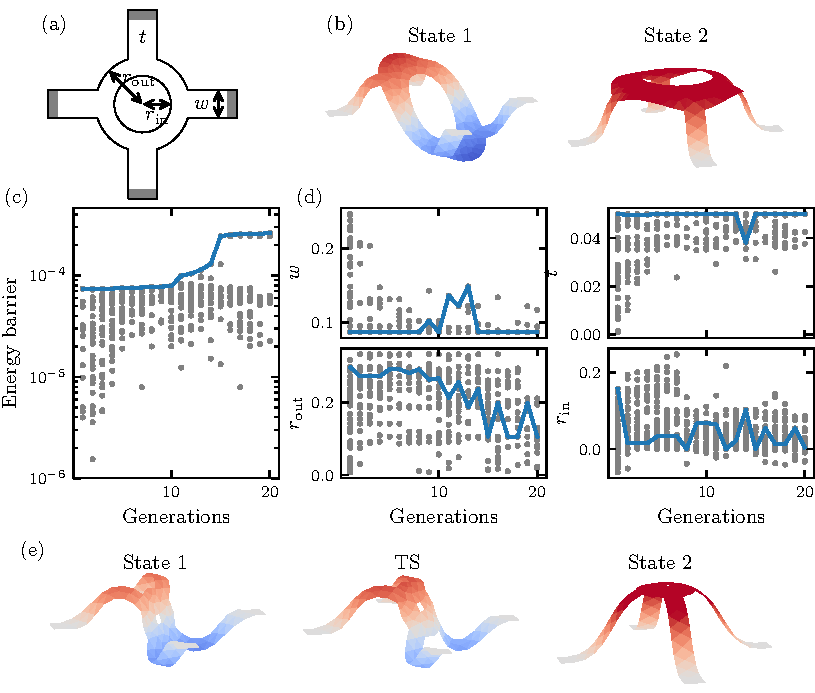
\includegraphics{structopt.pdf}
  \caption{\label{fig:ell-structopt}
    (a) Schematic of the structure showing the four parameters: leg width, $w$, thickness, $t$, outer radius, $r_\text{out}$, and inner radius, $r_\text{in}$.
        The fixed bonding sites are shown in grey.
    (b) The two minima for the structure with the highest barrier in the first generation.
        The colour represents the height above the horizontal plane, positive height in red, negative in blue.
    (c) The energy barrier for each individual in the population.
        The blue line follows the states with the highest barrier in each generation.
    (d) The values for each of the four parameters for each individual throughout the optimisation process.
        The parameters are scaled such that the total length of the structure, excluding bonding sites, is 1.
    (e) The minima and transition state for the most optimal state after 20 generations.
  }
\end{figure}

The results in \cref{fig:ell-structopt} show how the optimal structure evolves over time.
The leg width and thickness very quickly converge to their lower and upper bounds, respectively, and the inner radius also becomes small early on.
However, the outer radius takes more time to evolve, beginning with a large value, and only changing to a small radius around generation 15, at which point the maximum barrier correspondingly increases.
After 20 generations the optimal structure is: $w=0.0866$, $t=0.05$, $r_\text{out}=0.1145$, and $r_\text{in}=0.0137$.

These results demonstrate that a highly complex optimisation study is feasible using ELLib, and more generally, illustrates the flexibility of the library.

\begin{table}[]
  \begin{tabularx}{\textwidth}{>{\hsize=.5\hsize\linewidth=\hsize}C >{\hsize=.75\hsize\linewidth=\hsize}C >{\hsize=2\hsize\linewidth=\hsize}C >{\hsize=.75\hsize\linewidth=\hsize}C}
    \hline\hline
    Topic & Symbol & Parameter description & Value \\
    \hline
    \multirow{5}{*}{\rotatebox[origin=c]{90}{Structure}}
          & ---   & Compressive strain     & 20\% \\
          & ---   & Total structure length & 1 \\
          & ---   & Mesh resolution        & 0.05 \\
          & $Y$   & Young's modulus        & 1.4 \\
          & $\nu$ & Poisson ratio          & 0.3 \\
    \hline
    \multirow{5}{*}{\rotatebox[origin=c]{90}{BITSS}}
          & $\alpha$ & Energy constraint strength         & 10 \\
          & $\beta$  & Distance constraint error          & 0.1 \\
          & $f$      & Distance reduction factor          & 0.15 \\    
          & ---      & Coefficient calculation regularity & 100 iterations \\    
          & ---      & Max BITSS iterations               & 30 \\    
    \hline
    \multirow{5}{*}{\rotatebox[origin=c]{90}{\parbox{1.5cm}{\centering Genetic\\Algorithm}}}
          & ---      & Population size       & 48 \\
          & ---      & Number of generations & 20 \\
          & ---      & Mutation rate         & 0.25 \\    
          & ---      & Parent selection rate & 0.4 \\    
          & ---      & Pertubation size      & 30\% \\    
    \hline
    \hline\hline
  \end{tabularx}
  \caption{\label{tab:ell-params}
    Values of the parameters that are used in this section.
  }
\end{table}

  \chapter{3D Buckled Mesostructures}
\label{ch:mesostructures}
\graphicspath{{mesostructures/fig/}}

This chapter is based upon the joint work: Y. Li, S. J. Avis, J. Chen, G. Wu, T. Zhang, H. Kusumaatmaja, and X. Wang, ``Reconfiguration of multistable 3D ferromagnetic mesostructures guided by energy landscape surveys'', \emph{Extreme Mech. Lett.}, 48, 101428 (2021).

In particular, the experimental ferromagnetic structures are the work of Y. Li, while the simulations and energy landscape analysis are my own work.


\section{Introduction}

Reconfigurable three-dimensional structures that can actively change their geometries and thereby their functionalities upon external stimuli (like mechanical forces, magnetic fields, hydration, and temperature) \cite{Overvelde2017,Filipov2015,Wehner2016,Kim2018,Gladman2016,Xie2010} are promising for a diverse range of applications including deployable solar panels \cite{Thesiya2015}, metamaterials \cite{Fu2011,Wang2017,Lee2020}, phononics \cite{Babaee2016,Deng2020}, biomedical devices \cite{Damdam2019,Anderson2017}, robotics \cite{Plitea2013,Tang2019,Gorissen2020}, metasurfaces \cite{Liu2019a,Wang2016}, and many others.
The design of reconfigurable structures usually relies on structural instabilities \cite{Chen2012,Jiang2019,Zareei2020}, stimuli-responsive constituent materials (like swellable gels, shape memory polymers and magnetic materials) \cite{Gladman2016,Lendlein2005,Kim2012,Novelino2020,Liu2019b}, or their heterogeneous combinations \cite{Ding2017}.

As discussed in \cref{sec:es-mesostructures}, structural instabilities of simple 2D patterns under compression have been exploited to produce 3D buckled mesostructures, and can be used to realise a diverse range of complex 3D functional architectures and electronics \cite{Xu2015,Zhang2015,Wang2019a,Jang2017,Lee2018a}.
Through elastically deforming the assembly platform in different time sequences (i.e., loading-path control), the 3D structures have been shown to morph into different shapes \cite{Fu2018,Pang2020}.
In addition to mechanical deformation, reconfigurable structures can also be realised through active materials including ferromagnetic composites \cite{Kim2018,Kim2019,Hu2018,Boncheva2005}, hydrogels \cite{Gladman2016}, shape memory polymers (SMPs) \cite{Xie2010,Wang2019a}, liquid crystal elastomers (LCEs) \cite{White2015}, and electrochemically active materials \cite{Xia2019}, which can change their shape upon external stimuli.

In recent years, an emerging attractive strategy to realise robust reconfigurable structures is to encode multiple stable states by design that do not require persistent external stimuli \cite{Song2019,Yang2019,ODonnell2020,Li2020}.
Each of these stable states is a local minimum in a complex energy landscape, and therefore only a temporary external stimulus is needed to guide the structure from one state to another, after which it will remain in that state.

Despite intensive studies, a number of critical challenges remain, especially when asymmetric and complicated modes are involved in the architectural reconfiguration.
The first challenge is associated with the presence of multiple local minimum configurations, which could affect the stability of the targeted stable state under perturbations (e.g., environmental noises) or trap the structure in an intermediate state during the process of reconfiguration.
For example, it is recently recognised by researchers that hidden local minimum configurations can destroy the designed pathway of deploying origami structures \cite{Na2015,Silverberg2015}.
Thus, it is crucial to provide means of manipulating the energy well depth of targeted configurations and eliminating unfavorable local minima in the design of reconfigurable structures.

The second challenge stems from the complexity of the transition paths from one local minimum state to another, especially when the two states are separated by other stable and transition states \cite{Groh2019,Virot2017,Marthelot2017,Medina2020,Panter2019}.
A recent work \cite{Panter2019} shows that the transition from a uniformly deformed cylindrical shell to a 9-dimple buckled pattern needs to pass 7 local minimum configurations, which cannot be achieved by directly applying local probes to the shell.
Complicated transition paths among local minima are also found in mechanical metamaterials, which further provides new design parameters to program the deformed configurations of the structures \cite{Medina2020}.

Finally, it is also very challenging to realise remote, locally controlled, and rapid reconfiguration of the deformed, highly nonlinear structures \cite{Fu2018,Luo2019}.
These challenges call for a new means of systematically surveying the energy landscapes of the multistable structures to probe and tailor the energy barrier height among different local minima.

In this chapter, we develop a set of strategies to address these challenges and to guide the design of ferromagnetic 3D mesostructures, which are developed by our collaborators.
The use of ferromagnetic materials enables remote and rapid reconfiguration among different stable states via a portable magnet, eliminating the need for mechanical stages to apply controlled, global deformations to the substrate, as used in previous works \cite{Fu2018,Pang2020}.
Thus providing opportunities for remote, tetherless shape morphing, which is advantageous for many applications, especially those that require shape morphing in enclosed or delicate environments such as robotics and biomedical devices.

Theoretically, we employ a discrete shell model \cite{Seung1988,Grinspun2003} and path-finding algorithms \cite{Panter2019,E2007} to conduct fundamental studies on the complicated energy landscapes of the 3D ferromagnetic structures.
We construct design phase diagrams showing how the available stable states sensitively depend on the essential material and geometrical parameters of the elastic structures.
Furthermore, the minimum energy reconfiguration paths between the stable states and their energy barriers are identified using a combination of our developed BITSS method and the string method \cite{E2007}.
A salient advantage of our approach is that it allows the computation of reconfiguration paths following the minimum energy pathways (MEPs) systematically without the need to assume a predefined path for the structural transformation.

Our methodology is versatile and is applied to design and realise reconfigurable structures with a wide range of geometries, including ribbons and structures that resemble tables, baskets, flowers, boxes, single and double beams.
In all cases, the theoretically predicted and experimentally realised shapes and reconfiguration paths are in excellent agreement.
We also demonstrate reconfiguration of structures fabricated from non-active materials that are locally patterned with ferromagnetic films, which significantly expands the design space and material libraries for reconfigurable structures.

% Based upon these results, we highlight some proof- applications that have created by our experimental collaborators.
To further demonstrate the versatility of these reconfigurable 3D ferromagnetic structures, we highlight a number of applications that have been created by our experimental collaborators.
This includes a reconfigurable light emitting system, which illustrates the capacity to integrate other functional components into the 3D structures.
Finally, magnetically actuated particle delivery is shown, which utilises the different reconfigurational modes of a table structure.



\section{Results}

\subsection{Phase diagram of stable states for a table structure}

\Cref{fig:ms-1}(a) schematically illustrates the assembly process of a 3D structure from ferromagnetic composite thin films via compressive buckling, and the architectural reconfiguration of the structure via magnetic actuation.
The ferromagnetic composite is prepared by homogeneously embedding hard NdFeB (neodymium-iron-boron) microparticles into a soft elastomer, polydimethylsiloxane (PDMS).
These are then patterned into 2D layouts using a CO2 laser, followed by their magnetization using impulse magnetic fields (about 2.7 T).
They are then attached to a prestretched elastomeric substrate using a very thin layer of superglue to generate strong bonding at select location on the 2D patterns.
Releasing the prestrain in the substrate leads to compressive forces on the 2D ferromagnetic pattern at the bonding sites and geometrically transforms the pattern into a 3D structure.
We define the 2D layout to lie on the $x$-$y$ plane so that its normal vector is in the $z$ direction.

\begin{figure}[H]
  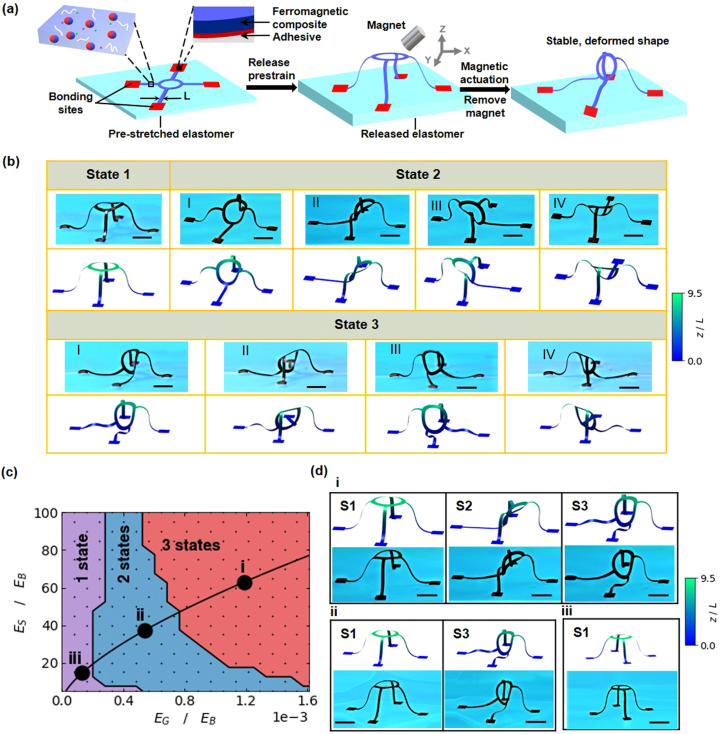
\includegraphics[width=\textwidth]{figure1.jpg}
  \caption{
    Multistability of magnetically reconfigurable 3D structures.
    (a) Schematic illustrating the assembly and reconfiguration of 3D ferromagnetic structures.
    (b) Experimental and computational results of multistable states in a 3D table structure.
    (c) Design phase diagram showing the number of distinct stable states based on the energy scales of the table structure.
        Representative examples in each regime with different values of $L$ are marked.
    (d) Experimental and computational results of the distinct stable states for the three representative examples marked in (c).
        S1-S3 refer to state 1-3, respectively.
    Scale bars, \SI{1}{\centi\meter}.
  }
  \label{fig:ms-1}
\end{figure}

To efficiently explore the possible stable states existing in the table structure, we simulate the structure using a simple discrete shell model.
The surface is discretised using a Delaunay triangulation \cite{Rebay1993}, with a target mesh size of a tenth of the ribbon width, and then the energy is calculated using the bar-and-hinge model discussed in \cref{sec:ell-bah}.
In these simulations, we assign the Young’s modulus of the ferromagnetic film to be $Y=\SI{1.4}{\mega\pascal}$ \cite{Kim2019} and use a thickness, $t=\SI{150}{\micro\meter}$.
The gravitational force is also included by setting the film density to its measured experimental value of $\rho = \SI{2.59}{\gram\per\centi\meter\cubed}$.
These parameters, and others used in this chapter, are listed in \cref{tab:or-params}.
Finally, we model the repulsive substrate interaction using a Lennard-Jones 3-9 potential with the attractive region removed.
Consequently, the model does not take into consideration the effect of adhesion which may become significant at small scales.

The stable states are obtained by minimizing the structures energy using the L-BFGS algorithm \cite{Nocedal1980,Liu1989}, which is highly efficient for minimization involving a large number of degrees of freedom.
The structures are buckled by steadily moving the binding sites from their positions in the flat precursor to their final positions over the first \num{10000} iterations.
While this buckling is taking place, the structure is split into a number of different regions and each is given a random force to enable the structure to take different configurations.
This process is repeated several hundreds of times to identify the different local minima in the energy landscape.

\Cref{fig:ms-1}(b) presents experimental and corresponding computational results of a 3D ferromagnetic table structure and its multiple stable states.
The table structure is oriented in a way such that gravity is perpendicular to the substrate (in the negative $z$ direction), which is the case for most of the structures in this study unless specified otherwise.

Three distinct states (state 1-3) with a total of nine configurations are discovered.
Magnetically deforming the assembled table structure via a portable disk magnet, with one leg becoming flat while the other three legs remain buckled, rapidly reconfigures the table structure from state 1 into a distinct stable state 2, with four different orientational configurations (state 2: shape I-IV).
Further magnetic actuation induces an additional leg of the table structure to become flat and results in the transition from state 2 into another stable state with four different orientations (state 3: shape I-IV).
In addition, unlike previously reported reconfigurable 3D structures that rely on persistent external stimuli to maintain their deformed shapes \cite{Kim2018,Gladman2016,White2015,Hajiesmaili2019}, the deformed configurations of the table structure shown here can well maintain their shapes after the applied magnetic field is removed, as they are locally stable configurations.
Computational modelling results of the configurations for the stable states and their different orientations via the discrete shell model are highly consistent with experiments, with the colour in the results denoting the displacement of the structure along the $z$ direction.

Using the combined experimental and computational strategy, we further study the effect of essential geometry and material properties on the entire spectrum of existing stable states, yielding the design phase diagram shown in \cref{fig:ms-1}(c).
The diagram illustrates the total number of stable states according to two dimensionless parameters that are determined from the ratios between three relevant energy scales – gravitational ($E_G$), stretching ($E_S$), and bending ($E_B$).
These energy scales can be expressed in terms of the material and geometric parameters of the 3D structure:
\begin{equation}
  E_G = \rho g L^3 t, \qquad E_S = Y L^2 t, \qquad E_B = \frac{Yt^3}{1-\nu^2},
\end{equation}
where $\rho$ is the material density, $Y$ is the Young’s modulus, $\nu$ is the Poisson ratio, $t$ is the film thickness, and $L$ represents the in-plane size of the structure (the width of table legs is used for this study).
The cubic term of $L$ in $E_G$ comes from the fact that the volume of the structure scales with $L^2$ and the displacement in the direction of gravity is proportional to $L$.

Three regimes in terms of the number of existing stable states can be identified in \cref{fig:ms-1}(c): (i) 3 distinct stable states, (ii) 2 distinct stable states, and (iii) 1 distinct stable state, which are controlled by two dimensionless variables $E_S/E_B = L^2(1-\nu^2)/t^2$ and $E_G/E_B = \rho g L^3 (1-\nu^2) / Yt^2$.
The variable $E_S/E_B$ characterises the bendability of the structure, with a larger value indicating that it is easier to generate bending deformation.
$E_G/E_B$ describes the competition between the gravitational and bending energies.
When $E_S/E_B$ and $E_G/E_B$ are relatively large, three distinct stable states as shown in \cref{fig:ms-1}(b) exist in regime i, with states 2 and 3 having 4 different orientations.
As the two dimensionless variables decrease, state 2 becomes unstable, resulting in two distinct stable states (states 1 and 3) for regime ii.
When $E_G/E_B$ is further reduced to an even smaller value, only the buckled-up state (state 1) is stable in regime iii.

To validate the phase diagram experimentally, we fabricate 3D ferromagnetic structures of the same film thickness ($t$) and material properties ($\rho$, $Y$, and $\nu$) but of different sizes ($L$), and magnetically reconfigure them into their multistable states.
\Cref{fig:ms-1}(d) (i-iii) demonstrates the number and configurations of the stable states for structures with $L = \SI{1.04}{\milli\meter}$, \SI{0.8}{\milli\meter}, and \SI{0.5}{\milli\meter}, respectively, which agree well with the prediction of the design phase diagram.
Please note that the overall in-plane dimensions of the structures are scaled proportionally with $L$ as it varies.

The diagram provides very important guidelines for achieving a well-controlled number of stable states or for removing undesired stable states in various applications by tuning the geometry and material properties.
For instance, if state 2 is undesired, the structure can be designed with $E_S/E_B$ and $E_G/E_B$ falling within regime ii, where only states 1 and 3 are stable.


\subsection{Reconfiguration pathways of a table structure}

Identifying the optimal transition pathways between the stable states of a 3D structure is critical for well-controlled, energy-efficient reconfigurations.
By using the table structure as an example, we further examine its energy landscape to identify the minimum energy pathways (MEPs) between metastable states, in which the maximum energy along the path occurs at a saddle point (the transition state).
However, the non-linear reconfigurations of the structure can thwart standard pathway methods unless they are initialised close to the correct path, and the large number of degrees of freedom used to model the structure can make the problem computationally intractable.
Instead, to locate the pathway efficiently, a combination of methods are used.
First, the transition state is located using the BITSS method, which does not require an initial pathway guess.
By minimising downhill from either side of the transition state with L-BFGS a pathway is generated, which is then refined using the string method (introduced in \cref{sec:lm-string}).

Our approach allows automatic and systematic computation of reconfiguration paths following the MEPs without the need to assume the pathways along which the structure morphs.
This is useful because the energy-efficient reconfiguration paths can be highly complex for 3D elastic structures, and it is not always possible to prescribe an expected pathway a priori, as typically adopted in previous works where energy barriers are calculated \cite{Fang2017,Fu2018,Virot2017,Shang2018}.

As shown in \cref{fig:ms-2}(a), we find the transition pathways to progress from state 3 to state 1 of the table structure can be broadly grouped into three regions: (I) two paths, 1 and 2, exist (red region); (II) two paths, 1 and 2*, exist (orange region); (III) only path 1 exists (yellow region).
The distinction between paths 2 and 2* is that the intermediate state 2 is no longer stable on the latter.
For illustration, we construct the design diagram by varying the in-plane size of the structures ($L$), while keeping their material properties ($\rho$, $Y$, and $\nu$) and film thickness ($t=\SI{125}{\micro\meter}$) constant.
The marked red and blue points correspond to those in the 3-state and 2-state regimes identified in the design diagram in \cref{fig:ms-1}(c), respectively.

For $L > \SI{0.89}{\milli\meter}$ (region I), two independent minimum energy pathways are found and illustrated in \cref{fig:ms-2}(b) for a representative table structure with $L = \SI{1.04}{\milli\meter}$.
The first (path 1) is a direct pathway with energy barrier $\upDelta E_1$, and the second (path 2), a path that passes through state 2 as an intermediary, with energy barriers $\upDelta E_2$ between states 3 and 2 and $\upDelta E_3$ between states 2 and 1.

\begin{figure}[H]
  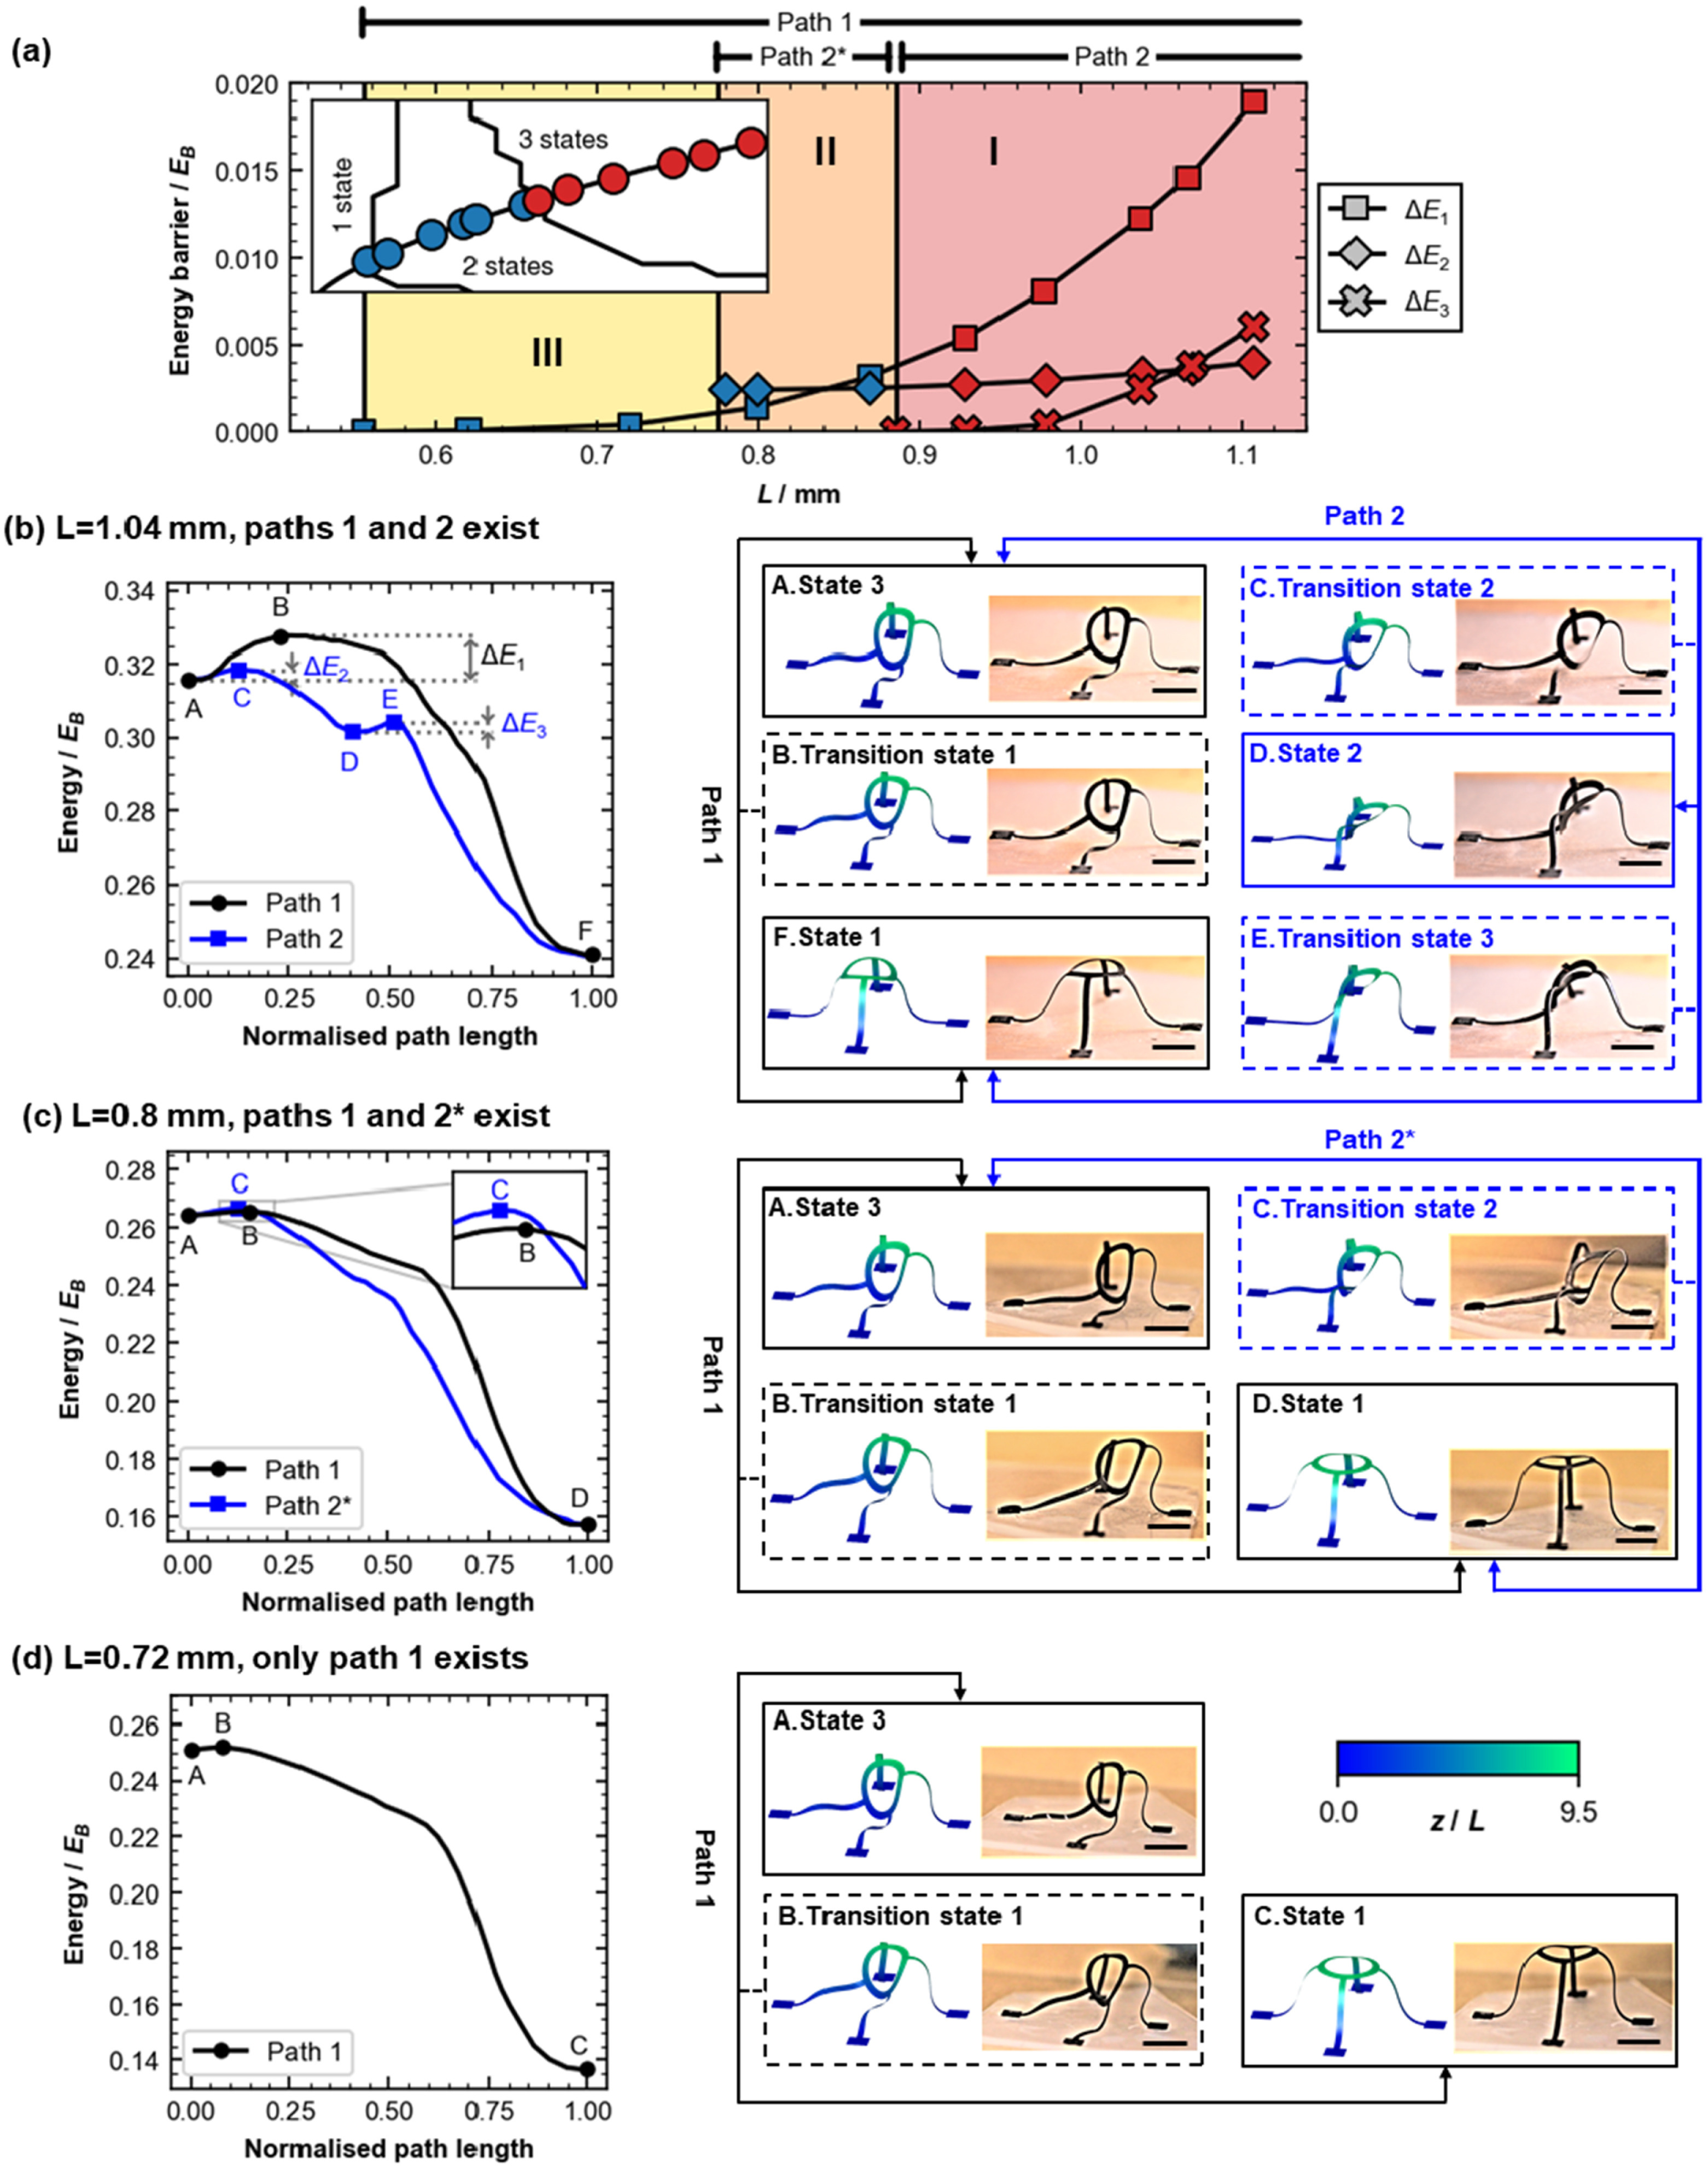
\includegraphics[width=\textwidth]{figure2.jpg}
  \caption{
    Energy barriers and reconfiguration pathways.
    (a) Variation of the energy barriers against $L$.
        Three regions (I-III) with different available pathways are highlighted.
        Inset: The locations within the design phase diagram.
    (b-d) Energy profiles and snapshots of stable and transition states for the pathways from state 3 to 1 with three values of $L$:
          (b) \SI{1.04}{\milli\meter}, (c) \SI{0.8}{\milli\meter}, and (d) \SI{0.72}{\milli\meter}.
          The energies are normalised by the bending energy.
          The definitions of the three energy barriers ($\upDelta E_1$, $\upDelta E_2$, $\upDelta E_3$) are shown in (b).
    Scale bars, \SI{1}{\centi\meter}.
  }
  \label{fig:ms-2}
\end{figure}

Snapshots of configurations along the pathways are captured in simulations and magnetic reconfiguration experiments and are shown in \cref{fig:ms-2}(b), with the complete structural transformation process and corresponding energy profiles simultaneously demonstrated in \cref{vid:pathA1,vid:pathA2}.

The energy barriers of the pathways demonstrate both the stability of the states and the ease of transitioning between them.
For example, the energy barrier to progress from state 3 to state 1 is much smaller than that from the inverse direction, thereby making state 1 more stable.
Comparing paths 1 and 2 also suggests that a smaller input energy is needed when reconfiguring the table structure along path 2 (passing two saddle points) than that along path 1.
However, the finite energy barrier $\upDelta E_3$ also indicates that the transition can be potentially trapped in state 2 if insufficient external energy is provided for reconfiguration.
In addition, reconfiguration along path 2 requires more efforts in manipulating the direction and the strength of external magnetic forces, compared to the direct pathway following path 1.

These complexities clearly show the importance of harnessing the energy landscape analysis for guiding the choice of transition paths based on specific applications and the nature of available external magnetic fields (or other external stimuli).
In addition, it is also worth noting that the pathways observed in experiments, where a portable magnet is utilised to reconfigure the structure from state 3 to state 1, are highly consistent with those from simulations, which indicates the high fidelity and reliability of the approach used in this study.
Moreover, the experimental reconfigurations can be completed within a few seconds (\cref{vid:pathA1,vid:pathA2}).
Such fast and remotely controlled transitions are desired for numerous applications, such as in soft robotics \cite{Tang2020,Alapan2020} and multifunctional metasurfaces \cite{Liu2019a,Wang2016}.

As we decrease $L$, all the energy barriers become smaller monotonically, as shown in \cref{fig:ms-2}(a).
At $L = \SI{0.89}{\milli\meter}$, the boundary between the 3-state and the 2-state regimes in the phase diagram of \cref{fig:ms-1}(c) is reached, where $\upDelta E_3$ reduces to zero, a signature that state 2 is no longer stable.
For $\SI{0.78}{\milli\meter} < L < \SI{0.89}{\milli\meter}$ (region II in \cref{fig:ms-2}(a)), there remains two distinct minimum energy pathways to transition from state 3 to state 1, even in the absence of a stable state 2.
The typical energy profiles for this range of $L$ values are illustrated in \cref{fig:ms-2}(c) for $L = \SI{0.80}{\milli\meter}$.
Snapshots of the configurations from simulations and experiments for $L = \SI{0.80}{\milli\meter}$ are further shown in \cref{fig:ms-2}(c), with reconfiguration along the full pathways provided in \cref{vid:pathB1,vid:pathB2}.
The shape evolution along the pathways remains qualitatively similar to that shown in \cref{fig:ms-2}(b).

Interestingly, we also find that there is a crossover in the preferred energy-efficient pathway at $L = \SI{0.84}{\milli\meter}$, where $\upDelta E_1 = \upDelta E_2$ in \cref{fig:ms-2}(a).
For a larger $L$ ($\SI{0.84}{\milli\meter} < L < \SI{0.89}{\milli\meter}$), path 2* is favorable because the corresponding energy barrier is smaller, while for a smaller $L$ ($\SI{0.78}{\milli\meter} < L < \SI{0.84}{\milli\meter}$), path 1 has a lower energy barrier and thereby is desired.

The preference for path 1 at smaller $L$ values is further accentuated by the loss of path 2* as a minimum energy pathway for $\SI{0.56}{\milli\meter} < L < \SI{0.78}{\milli\meter}$ (region III in \cref{fig:ms-2}(a)).
For this range of $L$ values, we are unable to identify path 2* in simulations, as indicated by the lack of data points in \cref{fig:ms-2}(a).
Furthermore, attempts to experimentally reconfigure along this pathway fail, with the structure instead following path 1.
Therefore, only path 1 remains.
The typical energy profile for the transition along path 1 in this range of $L$ values is shown in \cref{fig:ms-2}(d) for $L = \SI{0.72}{\milli\meter}$, with the corresponding snapshots of the reconfiguration and the full pathway given in \cref{fig:ms-2}(d) and \cref{vid:pathC1}, respectively.
State 3 itself becomes unstable when $L$ is further reduced below \SI{0.56}{\milli\meter}, where we enter the 1-state regime.
At this point the energy barrier $\upDelta E_1$ becomes zero, as seen in \cref{fig:ms-2}(a).

Taken together, these highly nonlinear behaviors observed for the transition pathways make the energy landscape analysis a necessary tool for an efficient and robust design of the multistable configurations and the transition paths among them, which has not been systematically studied before for continuous 3D mesostructures.


\begin{figure}[htb]
  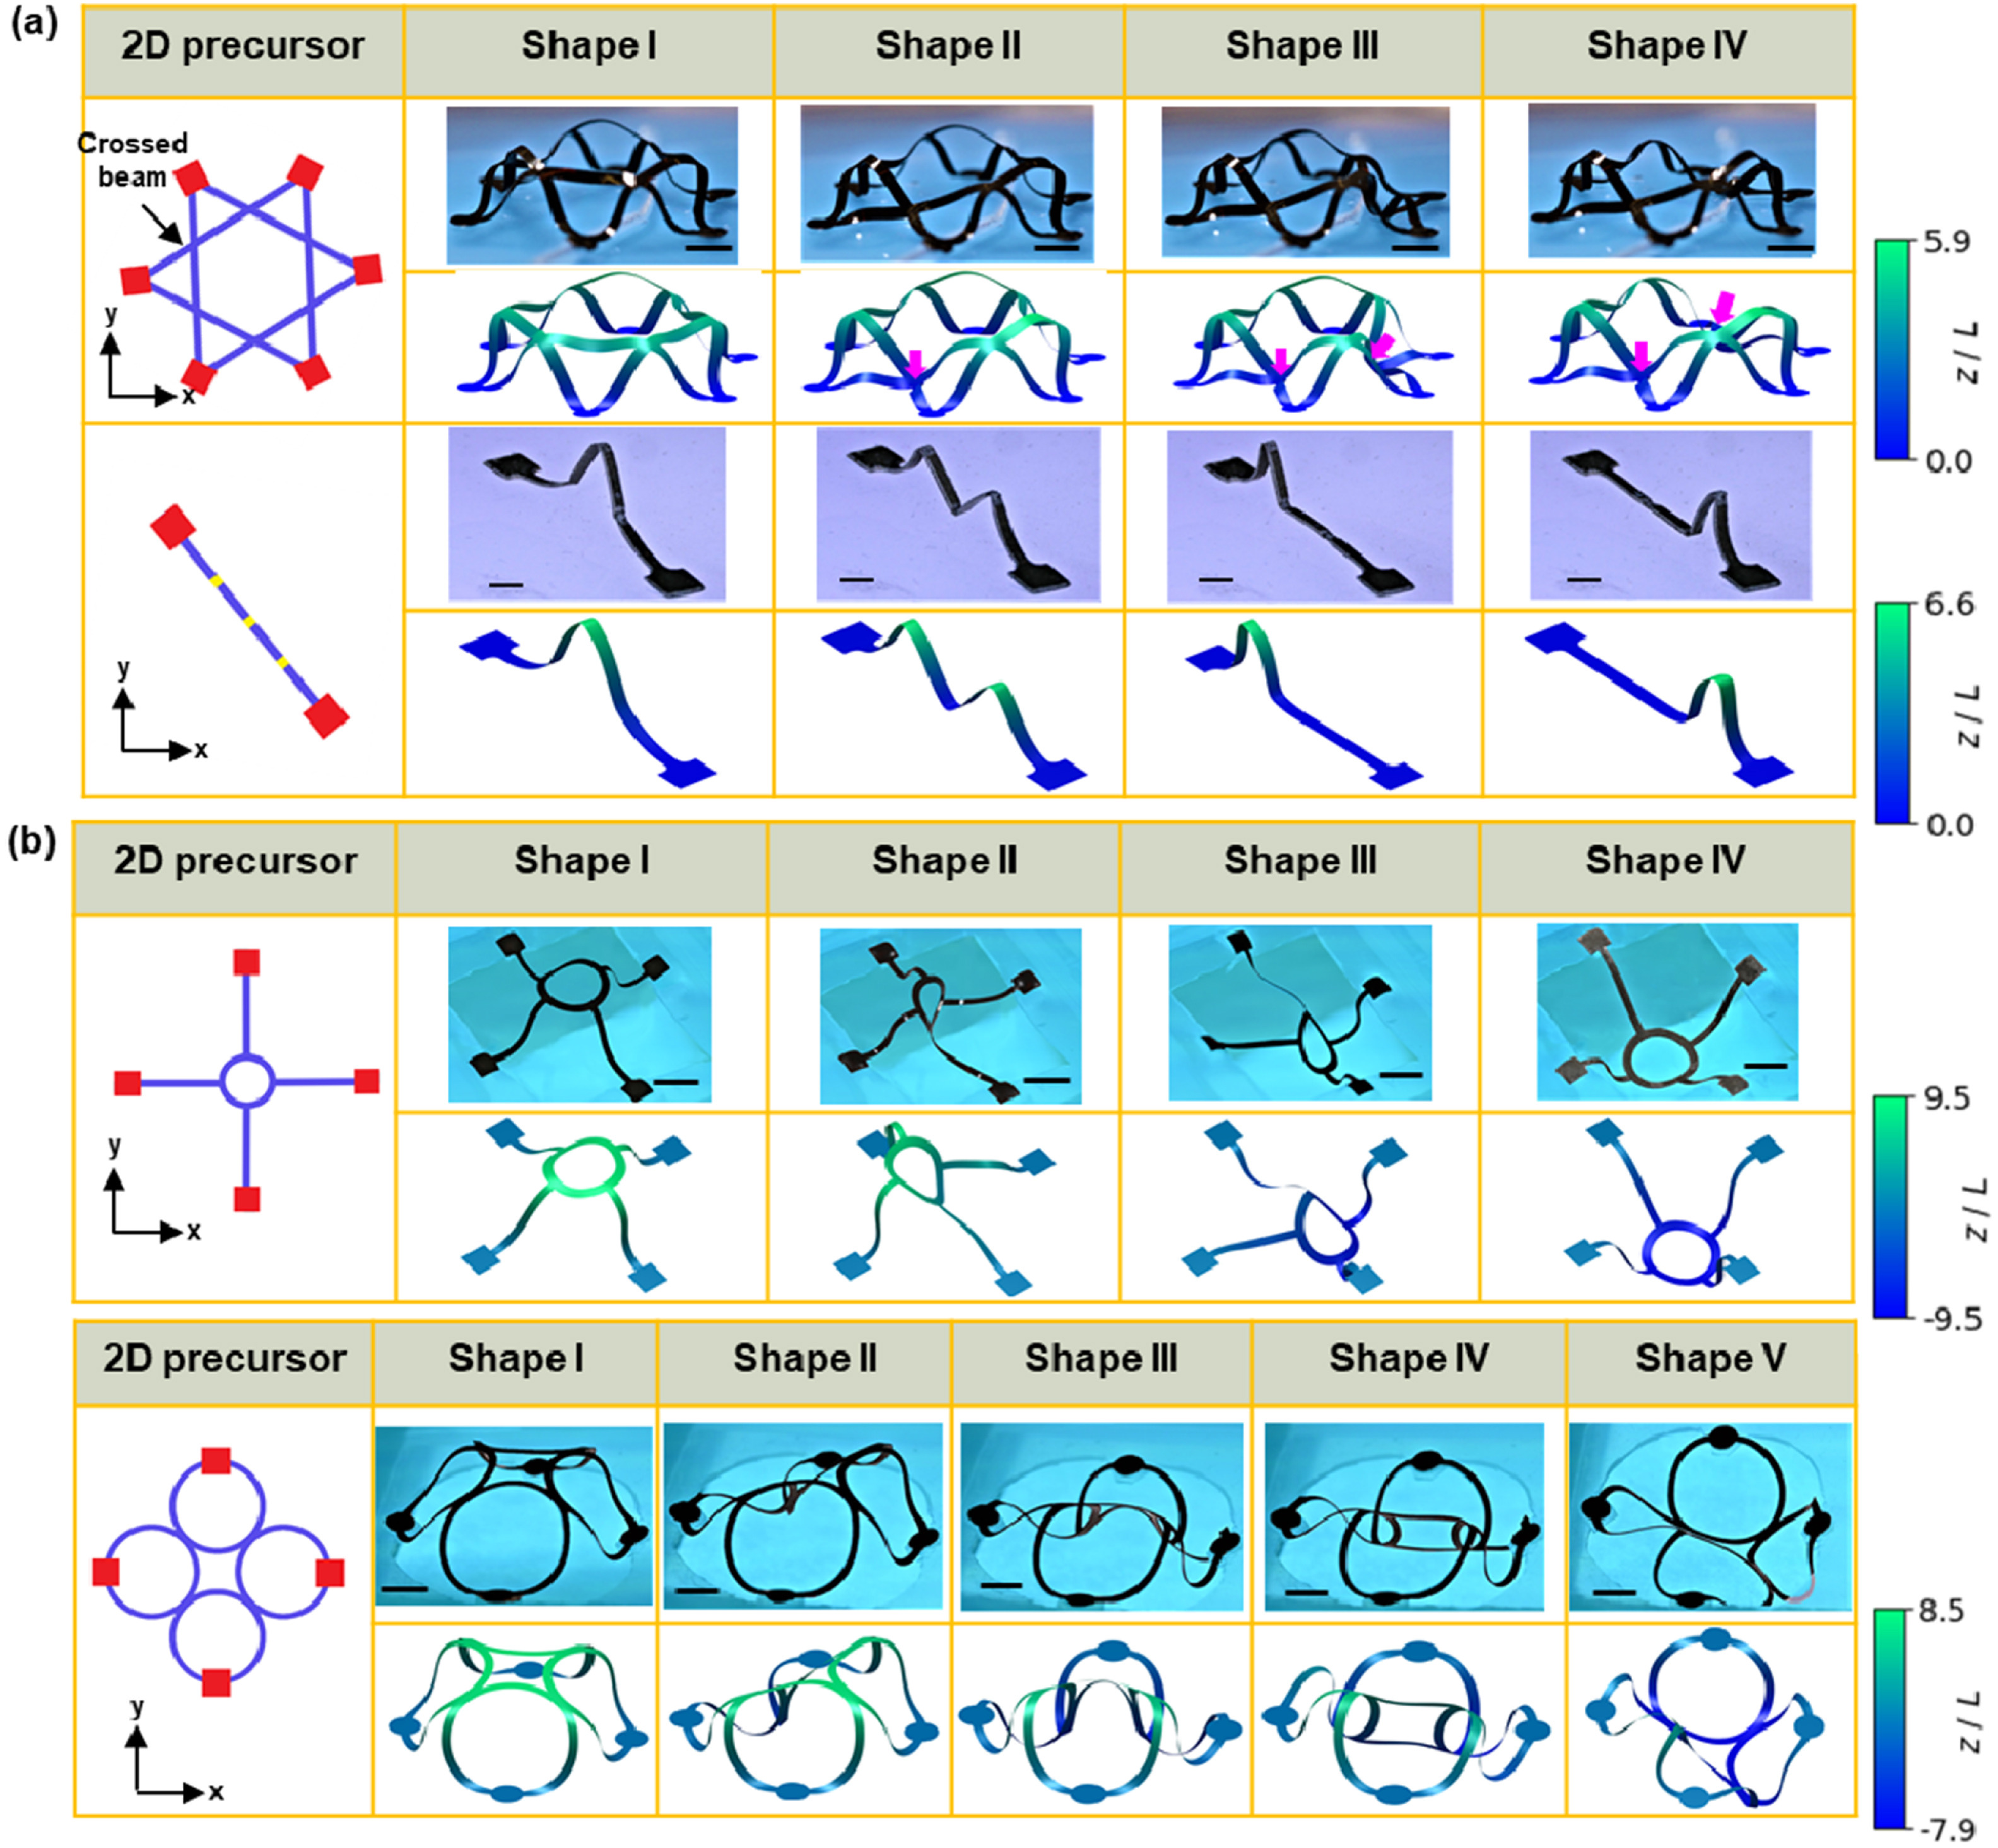
\includegraphics[width=\textwidth]{figure3.jpg}
  \caption{
    Diverse magnetically reconfigurable 3D structures.
    Optical images and computational modelling of multistable states for three types of structures:
    (a) 3D structures attached to a substrate.
        Pink arrows in the first structure indicate differences among the four shapes.
        Scale bars in the first and second structure are \SI{1}{\centi\meter} and \SI{2}{\milli\meter}, respectively.
    (b) 3D structures with the substrate underneath the structure removed.
        Scale bars, \SI{1}{\centi\meter}.
  }
  \label{fig:ms-3}
\end{figure}

\subsection{3D structures with diverse geometries}

The reconfiguration strategy and the energy landscape analysis described above are versatile and can be extended to different types of 3D structures in diverse geometries, as illustrated in \cref{fig:ms-3}.
\Cref{fig:ms-3}(a) shows an assembled ferromagnetic basket structure (shape I; film thickness: \SI{125}{\micro\meter}) and its multiple stable states (shapes II-IV) that can be achieved via magnetic control.
The pink arrows indicate differences among the four shapes.
In addition, by introducing creases to selective locations of a ribbon structure (crease thickness: \SI{70}{\micro\meter}; non-crease thickness: \SI{125}{\micro\meter}), we create a ferromagnetic origami structure, which is further tuned to display multiple stable configurations by using magnetic forces.

The elastomer substrate used for 3D assembly in \cref{fig:ms-1,fig:ms-2} provides essential support for the assembled 3D structures, but it also poses some limitations for the reconfiguration in the out of plane direction.
To allow more freedom for spatial reconfiguration, the substrate underneath the 3D table structure is removed, while the substrate adjacent to the bonding sites is maintained to support the 3D structure.
Such 3D structure on a hollow substrate allows bending up/down deformations across the plane of the substrate.
\Cref{fig:ms-3}(b) demonstrates a selection from a large variety of reconfigurable 3D structures on hollow substrates that have been investigated, including basket, single- and double-beam structures.

It is very interesting to note that the multistable configurations on hollow substates are sensitive to the orientation of the structures.
Take the table structure for example, when placed horizontally (i.e., the direction of gravity is perpendicular to the substrate), the structure only displays two stable states, buckled up and down.
However, when the table structure is placed vertically with the direction of gravity in the $x$ direction (\cref{fig:ms-3}(b)), in addition to the buckled up (Shape I) and down (Shape IV) states, it can deform into an asymmetric, twisted shape (Shape II), similar to state 3 of the table structure with an intact substrate.
This deformed shape can be further magnetically deformed into shape III, with the four bonding sites attached to the substrate and the rest of the structure self-supported in the air.

We also carry out energy landscape analysis for this structure, the details of which are presented in \cref{fig:ms-s6}.
Similar to the case with an intact substrate, we can distinguish several regimes with different numbers of stable states, depending on the three relevant energy scales: gravitational, stretching, and bending energies.

In addition, we quantitatively compare the dimensions of three representative 3D structures from experiments and modelling results and find negligible difference between them (\cref{tab:ms-comparison}), which further highlights the consistency between modelling and experimental results.

\begin{figure}[htb]
  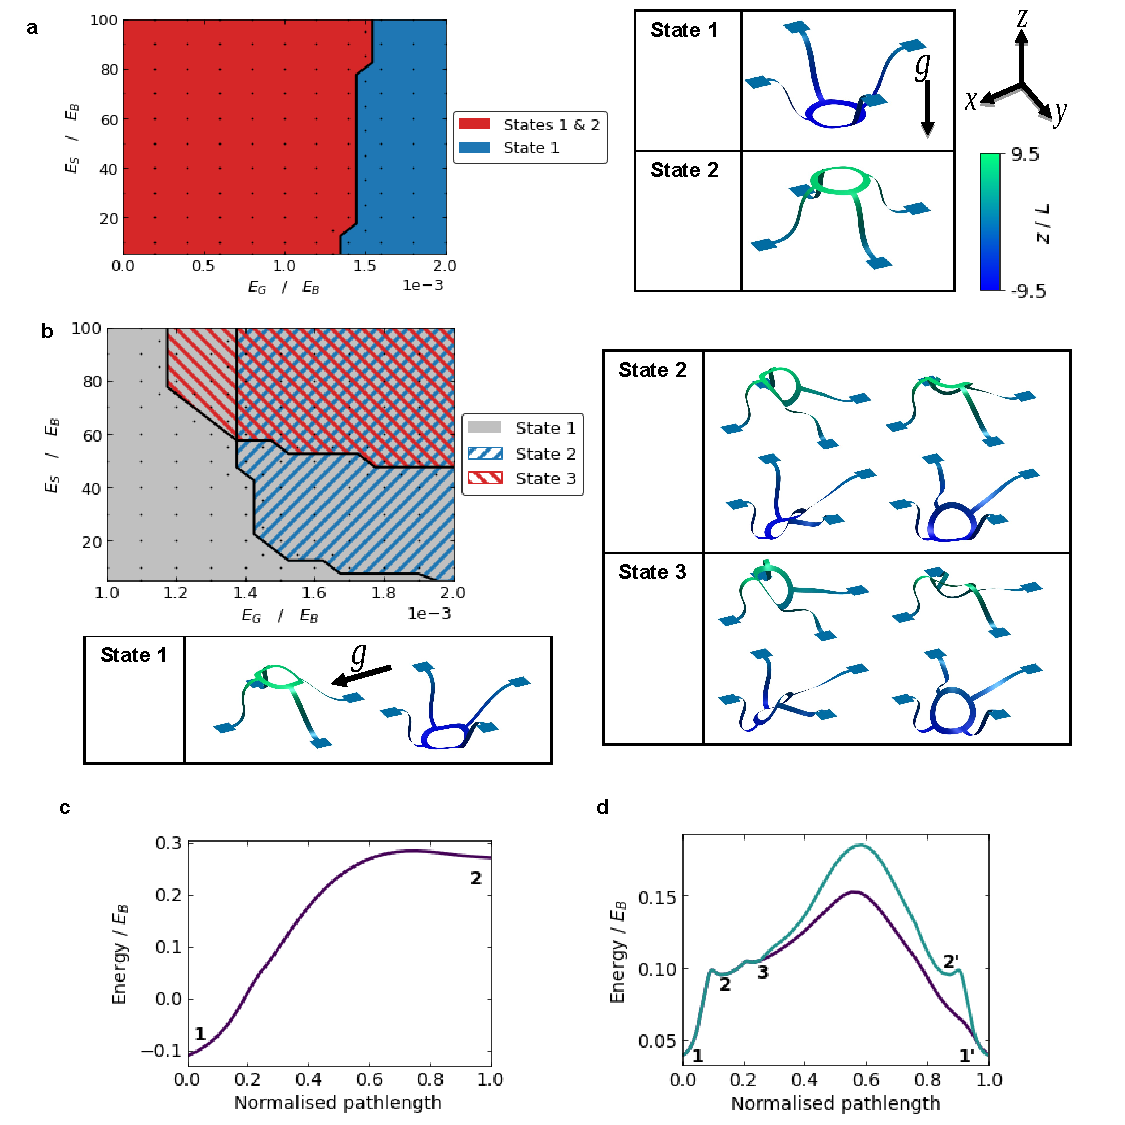
\includegraphics[width=\textwidth]{figureS6.pdf}
  \caption{
    (a-b) Phase diagrams of table structures on hollow substrates, with the direction of gravity in (a) the $z$-direction, (b) the $x$-direction.
          In panel (b), state I has two equivalent configurations, while both states II and III have four equivalent configurations.
    (c) Energy profile of the transition pathway from the buckled-down (state 1) to buckled-up (state 2) configurations when gravity is in the $z$-direction.
    (d) Energy profile of the transition pathway from the buckled-down (state 1) to buckled-up (state 1’) configurations when gravity is in the $x$-direction.
  }
  \label{fig:ms-s6}
\end{figure}

\begin{table}[htb]
  \setkeys{Gin}{width=\linewidth}
  \begin{tabularx}{\textwidth}{>{\centering}m{0.2\textwidth}CC >{\centering}m{0.2\textwidth}CC}
    \hline\hline
    \multicolumn{3}{c}{Experiment} & \multicolumn{3}{c}{Simulation} \\
    \cmidrule(lr){1-3}\cmidrule(lr){4-6}
    State & Width (mm) & Height (mm) & State & Width (mm) & Height (mm) \\
    \hline
    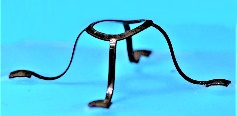
\includegraphics{comparison/experiment-1.png} & 32.2 & 9.2 &
    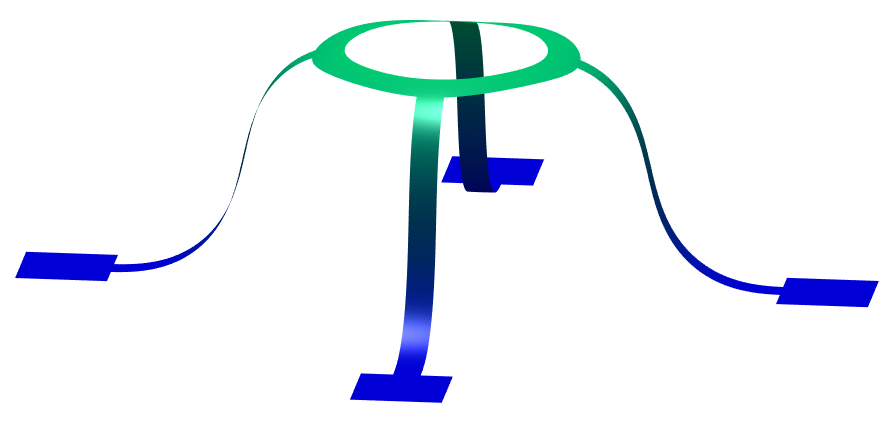
\includegraphics{comparison/simulation-1.png} & 33.5 & 9.0
    \\
    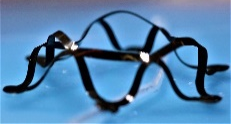
\includegraphics{comparison/experiment-2.png} & 37.6 & 10.7 &
    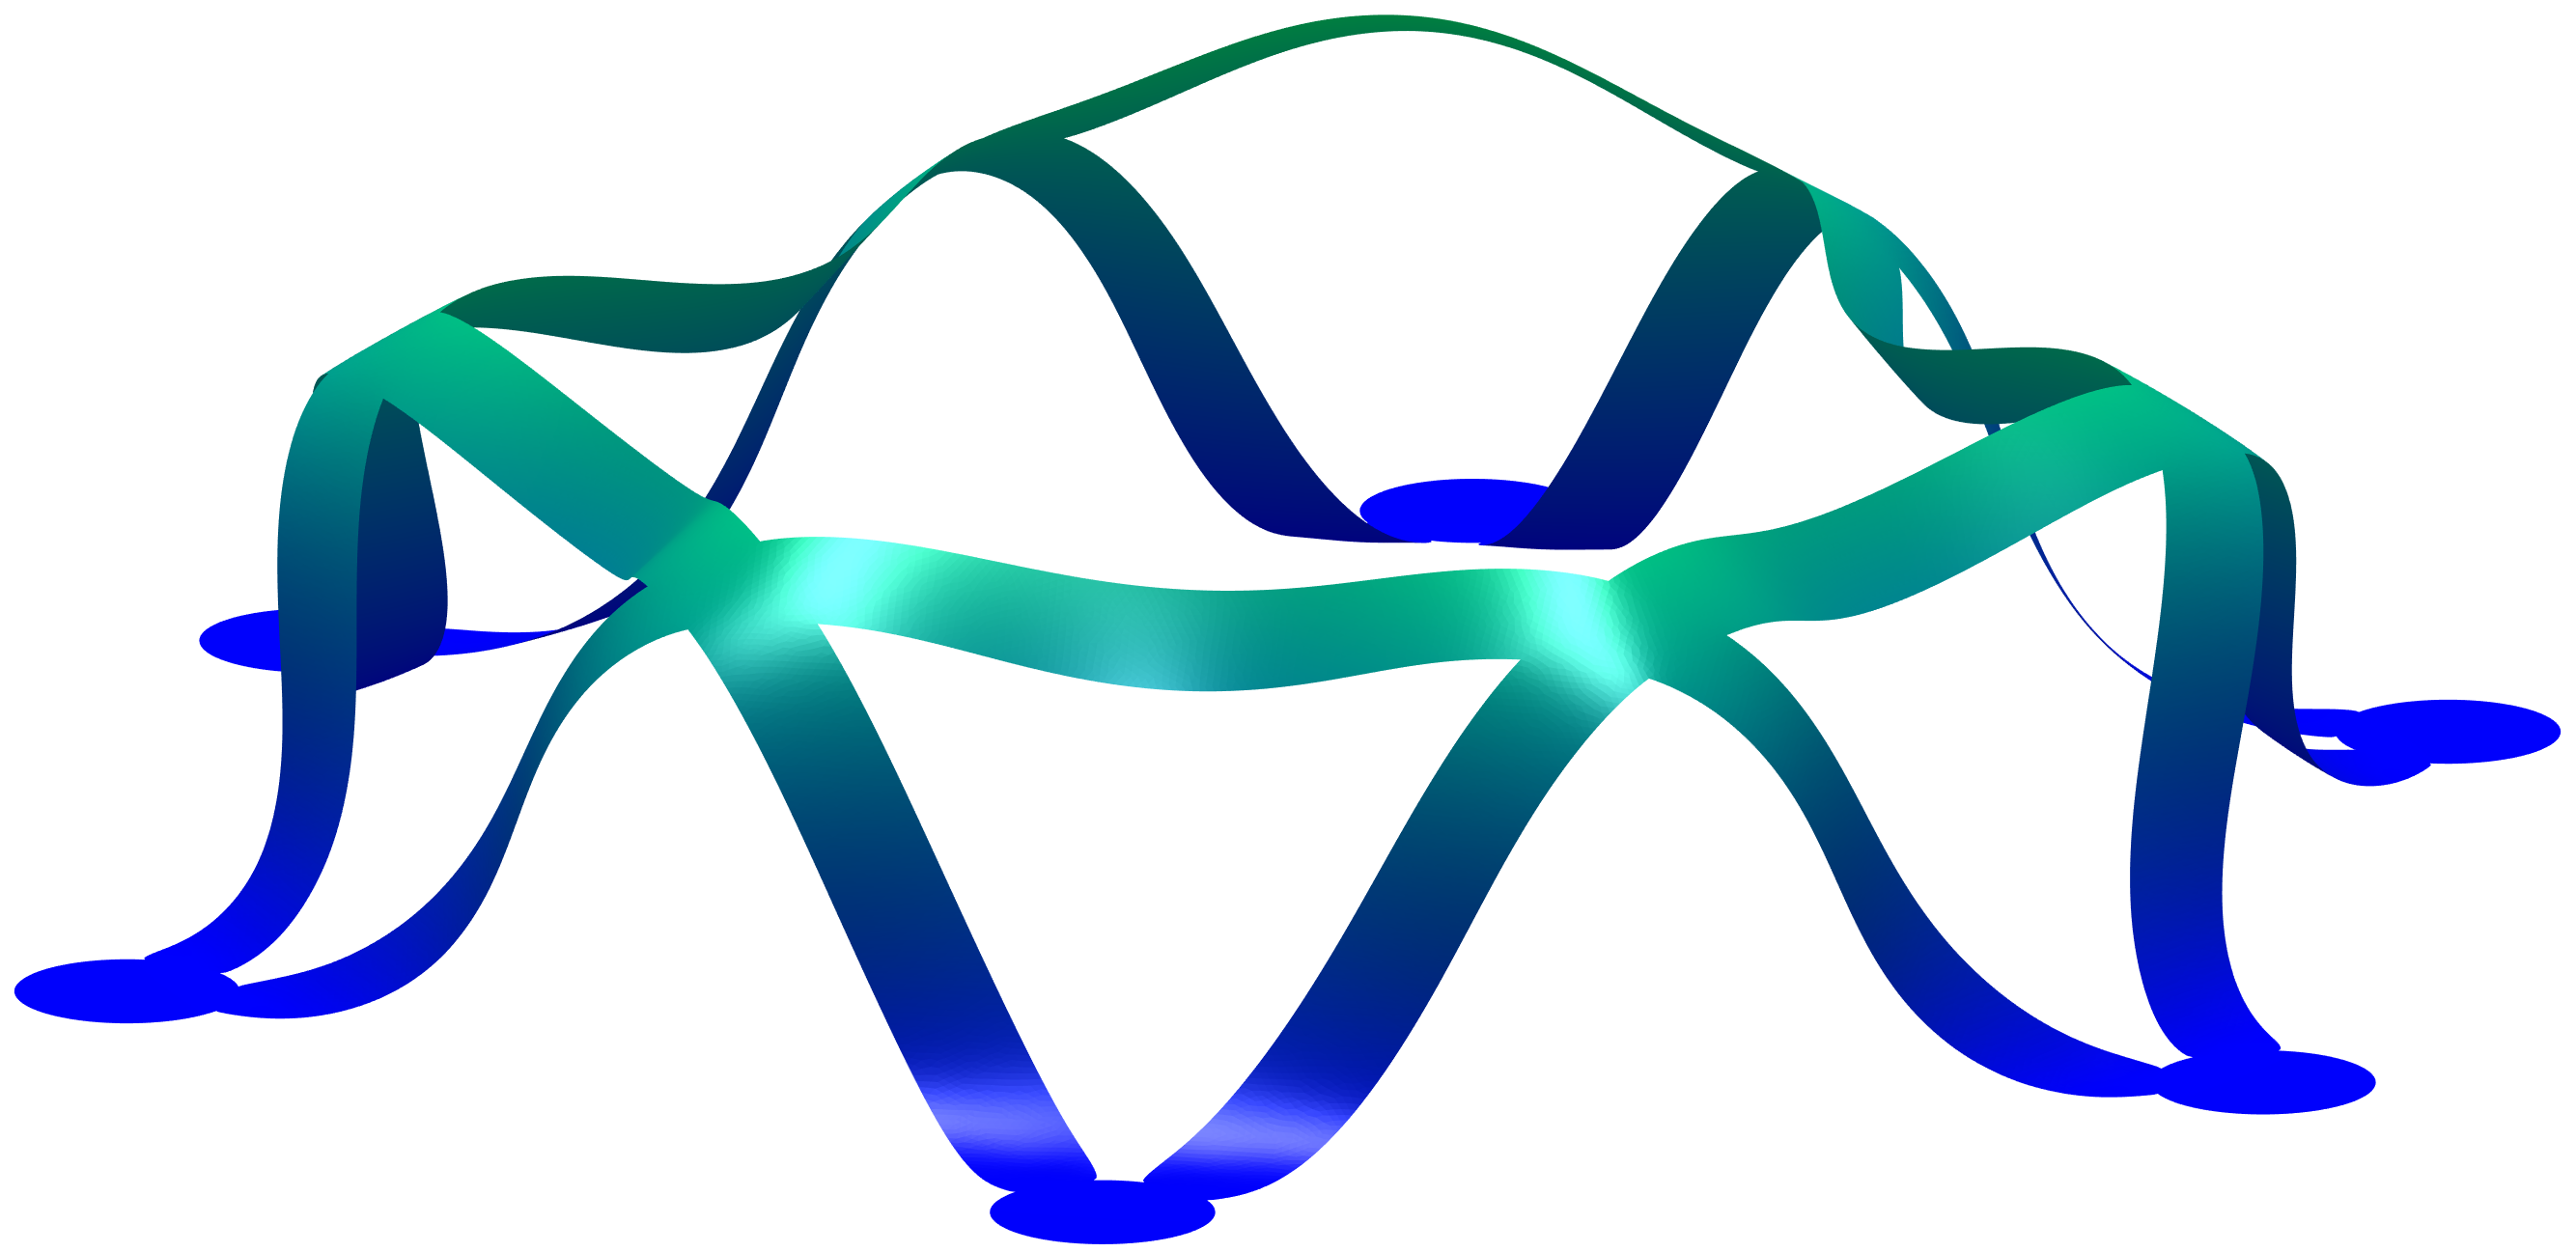
\includegraphics{comparison/simulation-2.png} & 38.0 & 10.9
    \\
    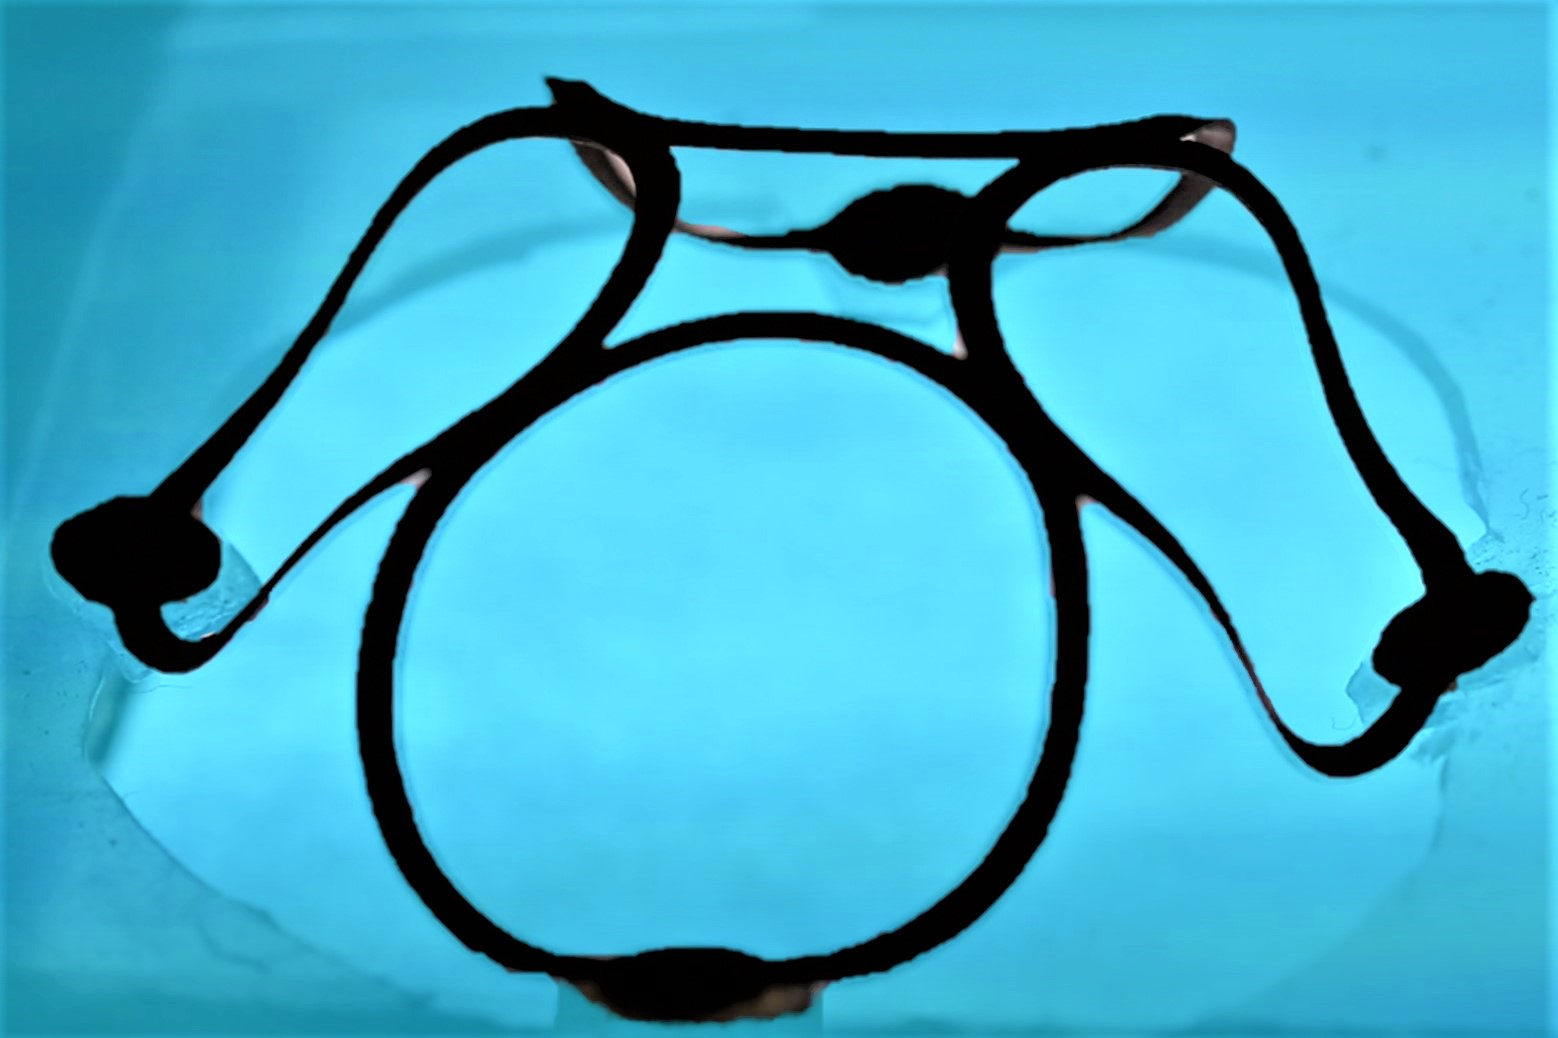
\includegraphics{comparison/experiment-3.png} & 31.5 & 10.1 &
    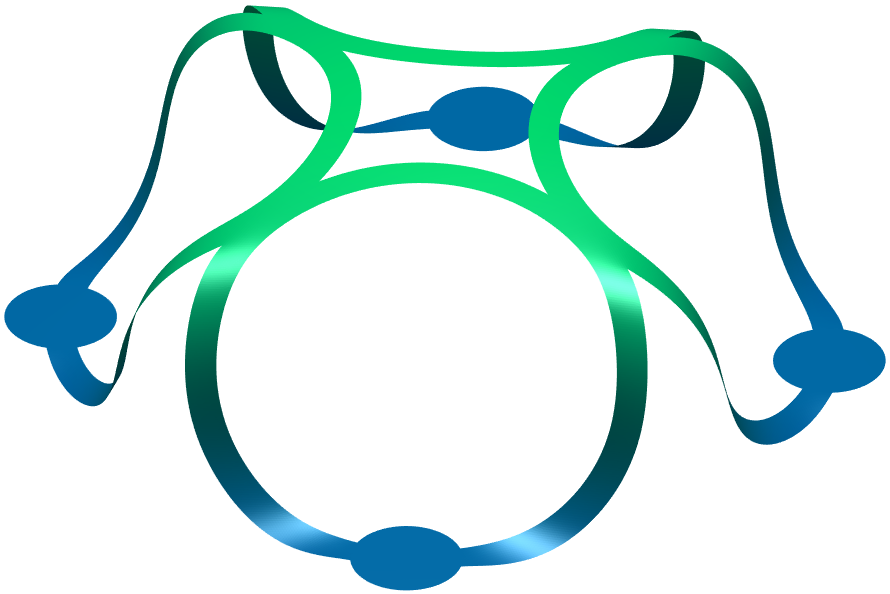
\includegraphics{comparison/simulation-3.png} & 31.9 & 9.9
    \\
    \hline\hline
  \end{tabularx}
  \caption{The dimension comparison of experimental 3D structures and simulated 3D structures.}
  \label{tab:ms-comparison}
\end{table}


\subsection{Hybrid ferromagnetic structures}

In addition to tuning the strength and the direction of external magnetic forces for reconfiguration, an alternative and potentially more versatile means to realise magnetically controlled reconfiguration is through manipulating the distribution of magnetic materials within 3D hybrid structures.
\Cref{fig:ms-4}(a) schematically illustrates the fabrication process of such structures by locally integrating laser-cut ferromagnetic composite film patches (\SI{125}{\micro\meter} thick) onto a thin layer of inactive materials (PDMS, \SI{180}{\micro\meter} thick) and compressively buckling the 2D hybrid pattern into a 3D structure.

Following this strategy, reconfigurable 3D hybrid structures that resemble tables and flowers are fabricated and magnetically tuned to display five stable configurations (Shape I-V) using a portable magnet.
The deformed shapes can well maintain their configuration after the magnetic force is removed, the capability of which is the same as structures composed of a single layer of ferromagnetic composites.

In addition, 3D hybrid structures can potentially allow more local magnetic control by varying the direction and the strength of the residual magnetic field in each ferromagnetic patch through magnetization in different directions and mixing different concentrations of magnetic particles in the composite film, respectively.
This could be combined with information from the energy landscape analysis in order to design the patches so the deformation in a magnetic field most accurately follows the MEP.
However, this analysis and the exploration of other composition materials for reconfigurable 3D hybrid structures are beyond the scope of the current work.

\begin{figure}[htb]
  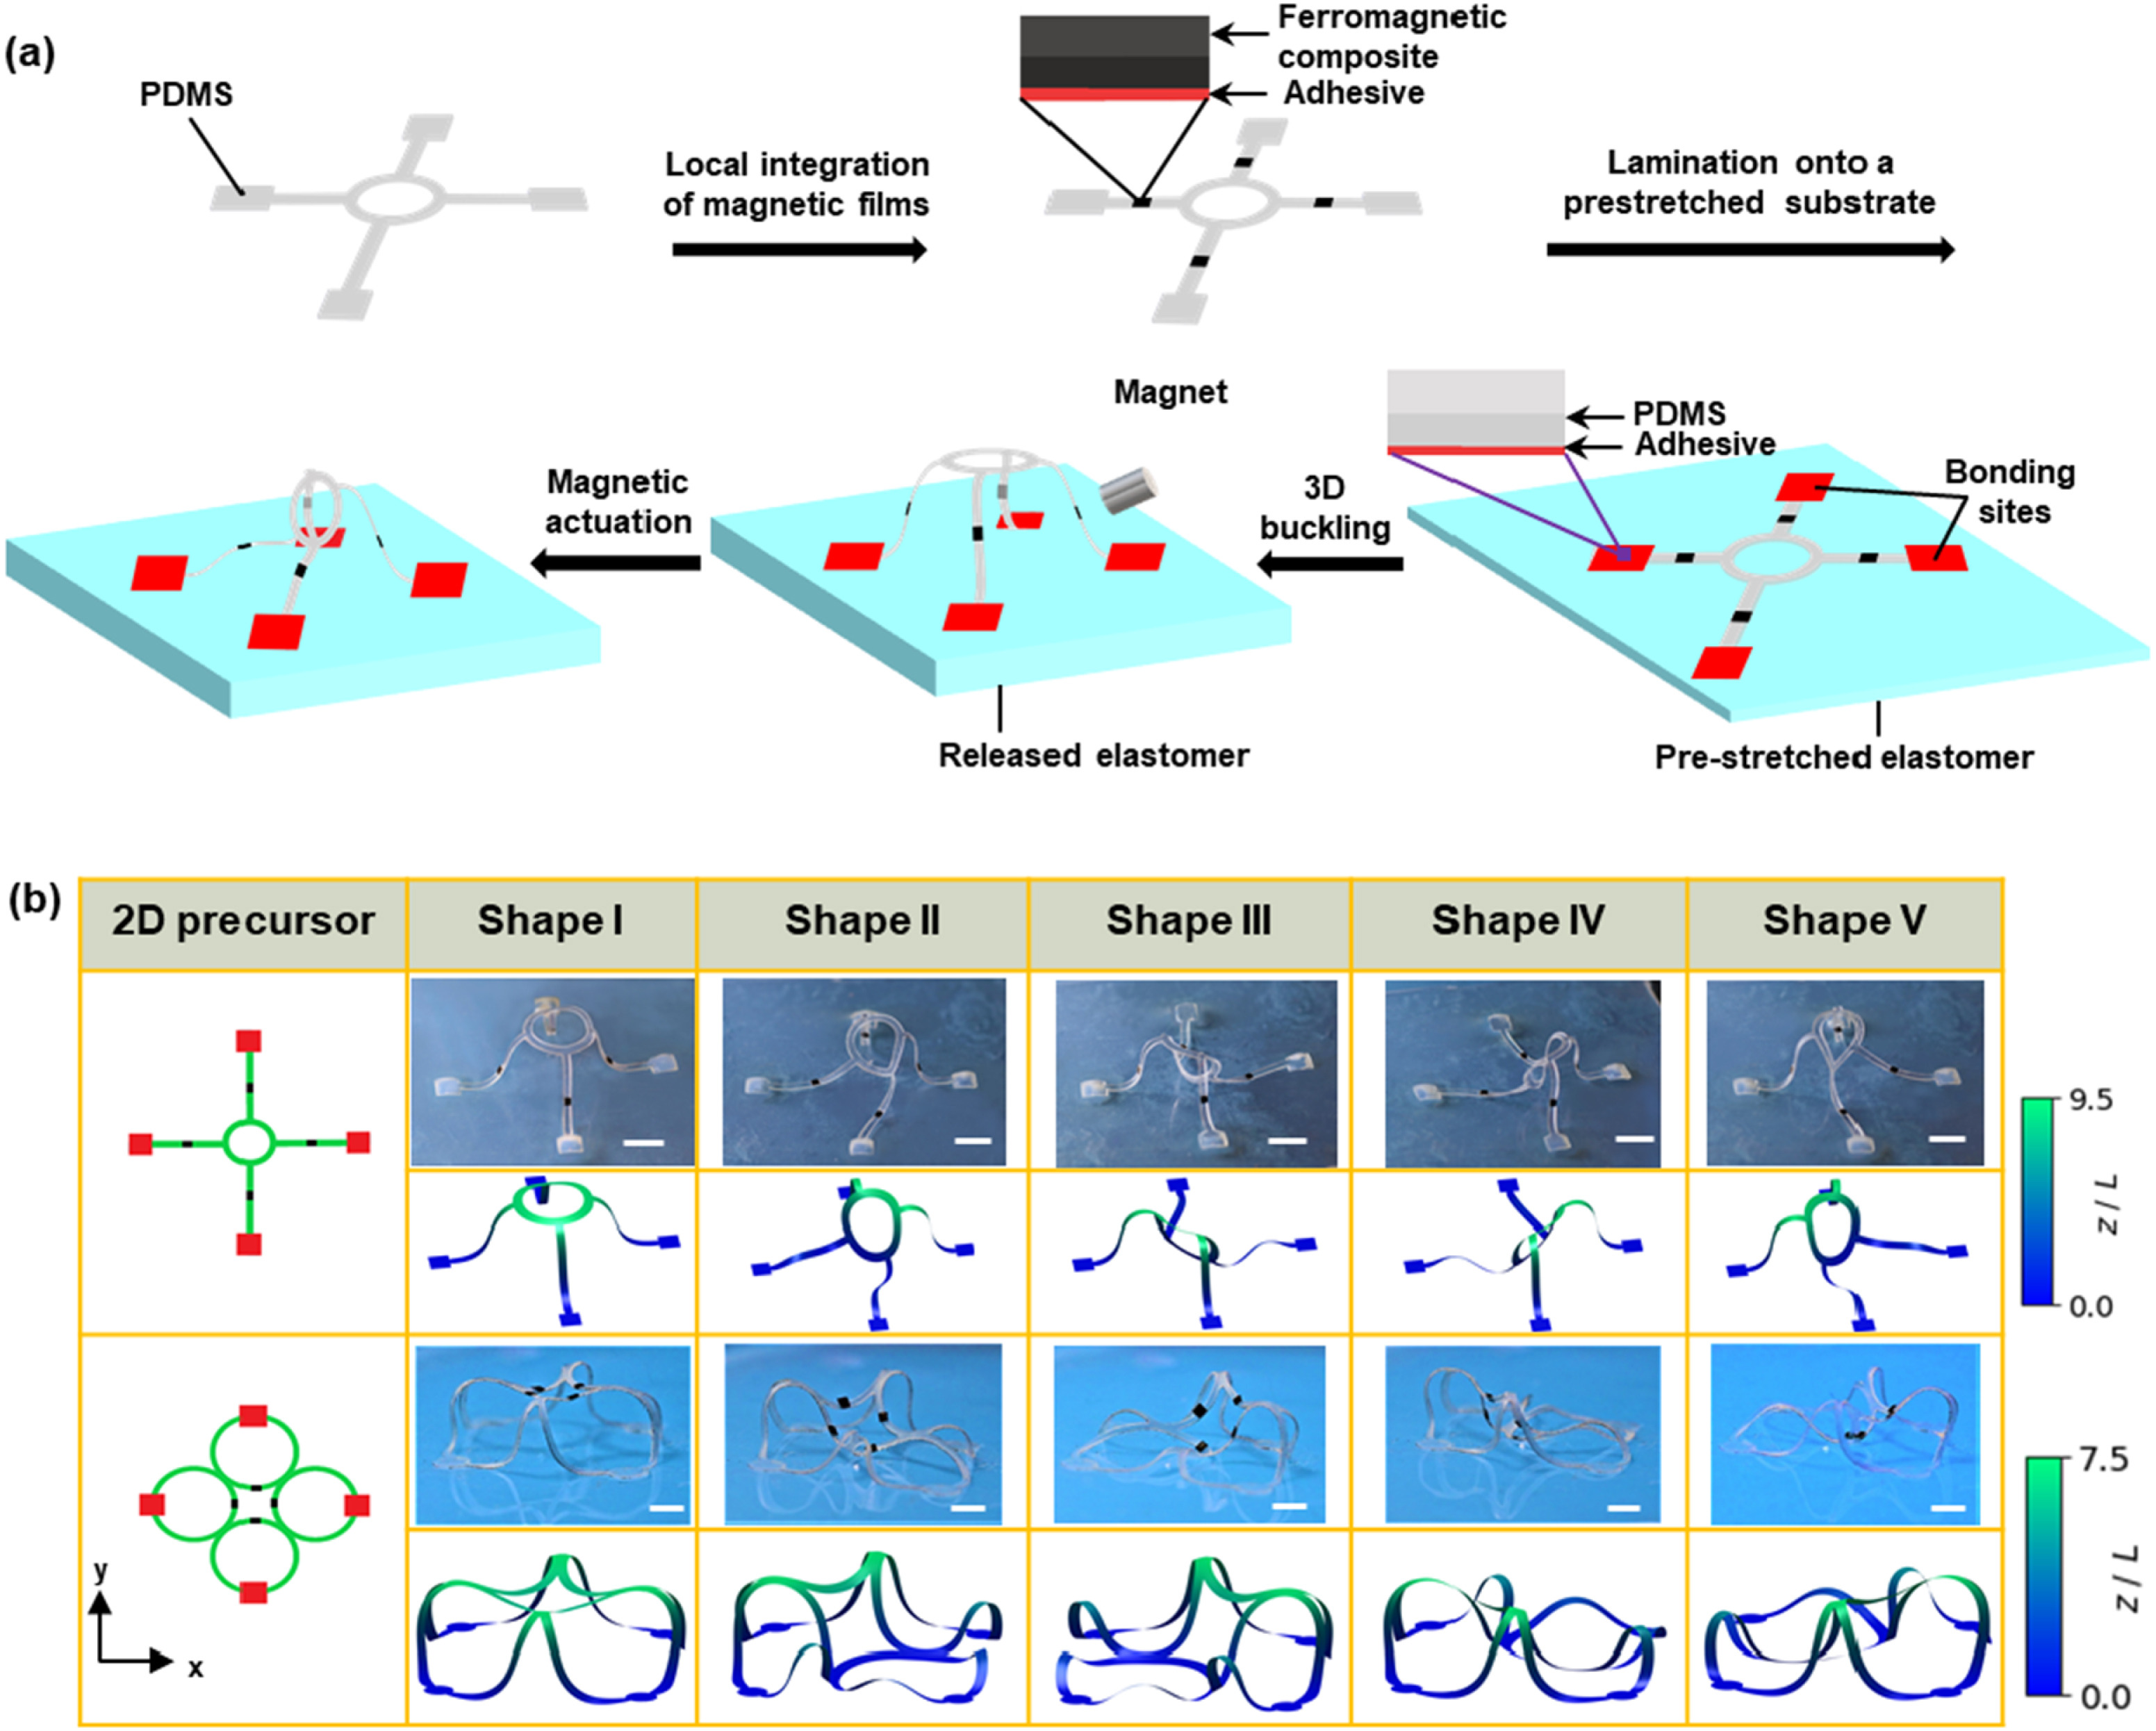
\includegraphics[width=\textwidth]{figure4.jpg}
  \caption{
    Locally tunable, heterogeneous 3D structures.
    (a) Schematic illustration of the fabrication process for locally controlled heterogeneous 3D ferromagnetic structures.
    (b) Optical images and computational modelling of multistable states for 3D structures composed of locally patterned ferromagnetic films on a thin layer of PDMS.
        Scale bars, \SI{1}{\centi\meter}.
  }
  \label{fig:ms-4}
\end{figure}


\subsection{Applications of reconfigurable 3D structures}
Using the techniques described above, our experimental collaborators have designed two proof-of-principle applications that demonstrate the potential offered by reconfigurable ferromagnetic mesostructures.

Firstly, functional materials and components may be integrated onto the 2D precursor, providing access to tunable 3D functional devices.
This is demonstrated using a reconfigurable light emitting system in \cref{fig:ms-5}(a).
Here, two light emitting diodes (LEDs) are integrated onto designated locations of a double-beam structure with copper thin films connected to the LED serving as contacts for LED activation.
The cross-links in the structure can be individually buckled using magnetic actuation, deforming the structure from shape I to II (or III).
This enables a firm contact between the LED on the structure with the copper contacts on the substrate, connecting to an external power supply and activating the LED.
The multistability of the structure then enables the LED to maintain its “on” status after the magnetic force is removed.
When the two beams are simultaneously deformed to form stable configuration IV using a magnet, both LEDs are turned on.
This simple example suggests a broad range of possibilities in other types of electronic and optoelectronic devices.

\begin{figure}[htb]
  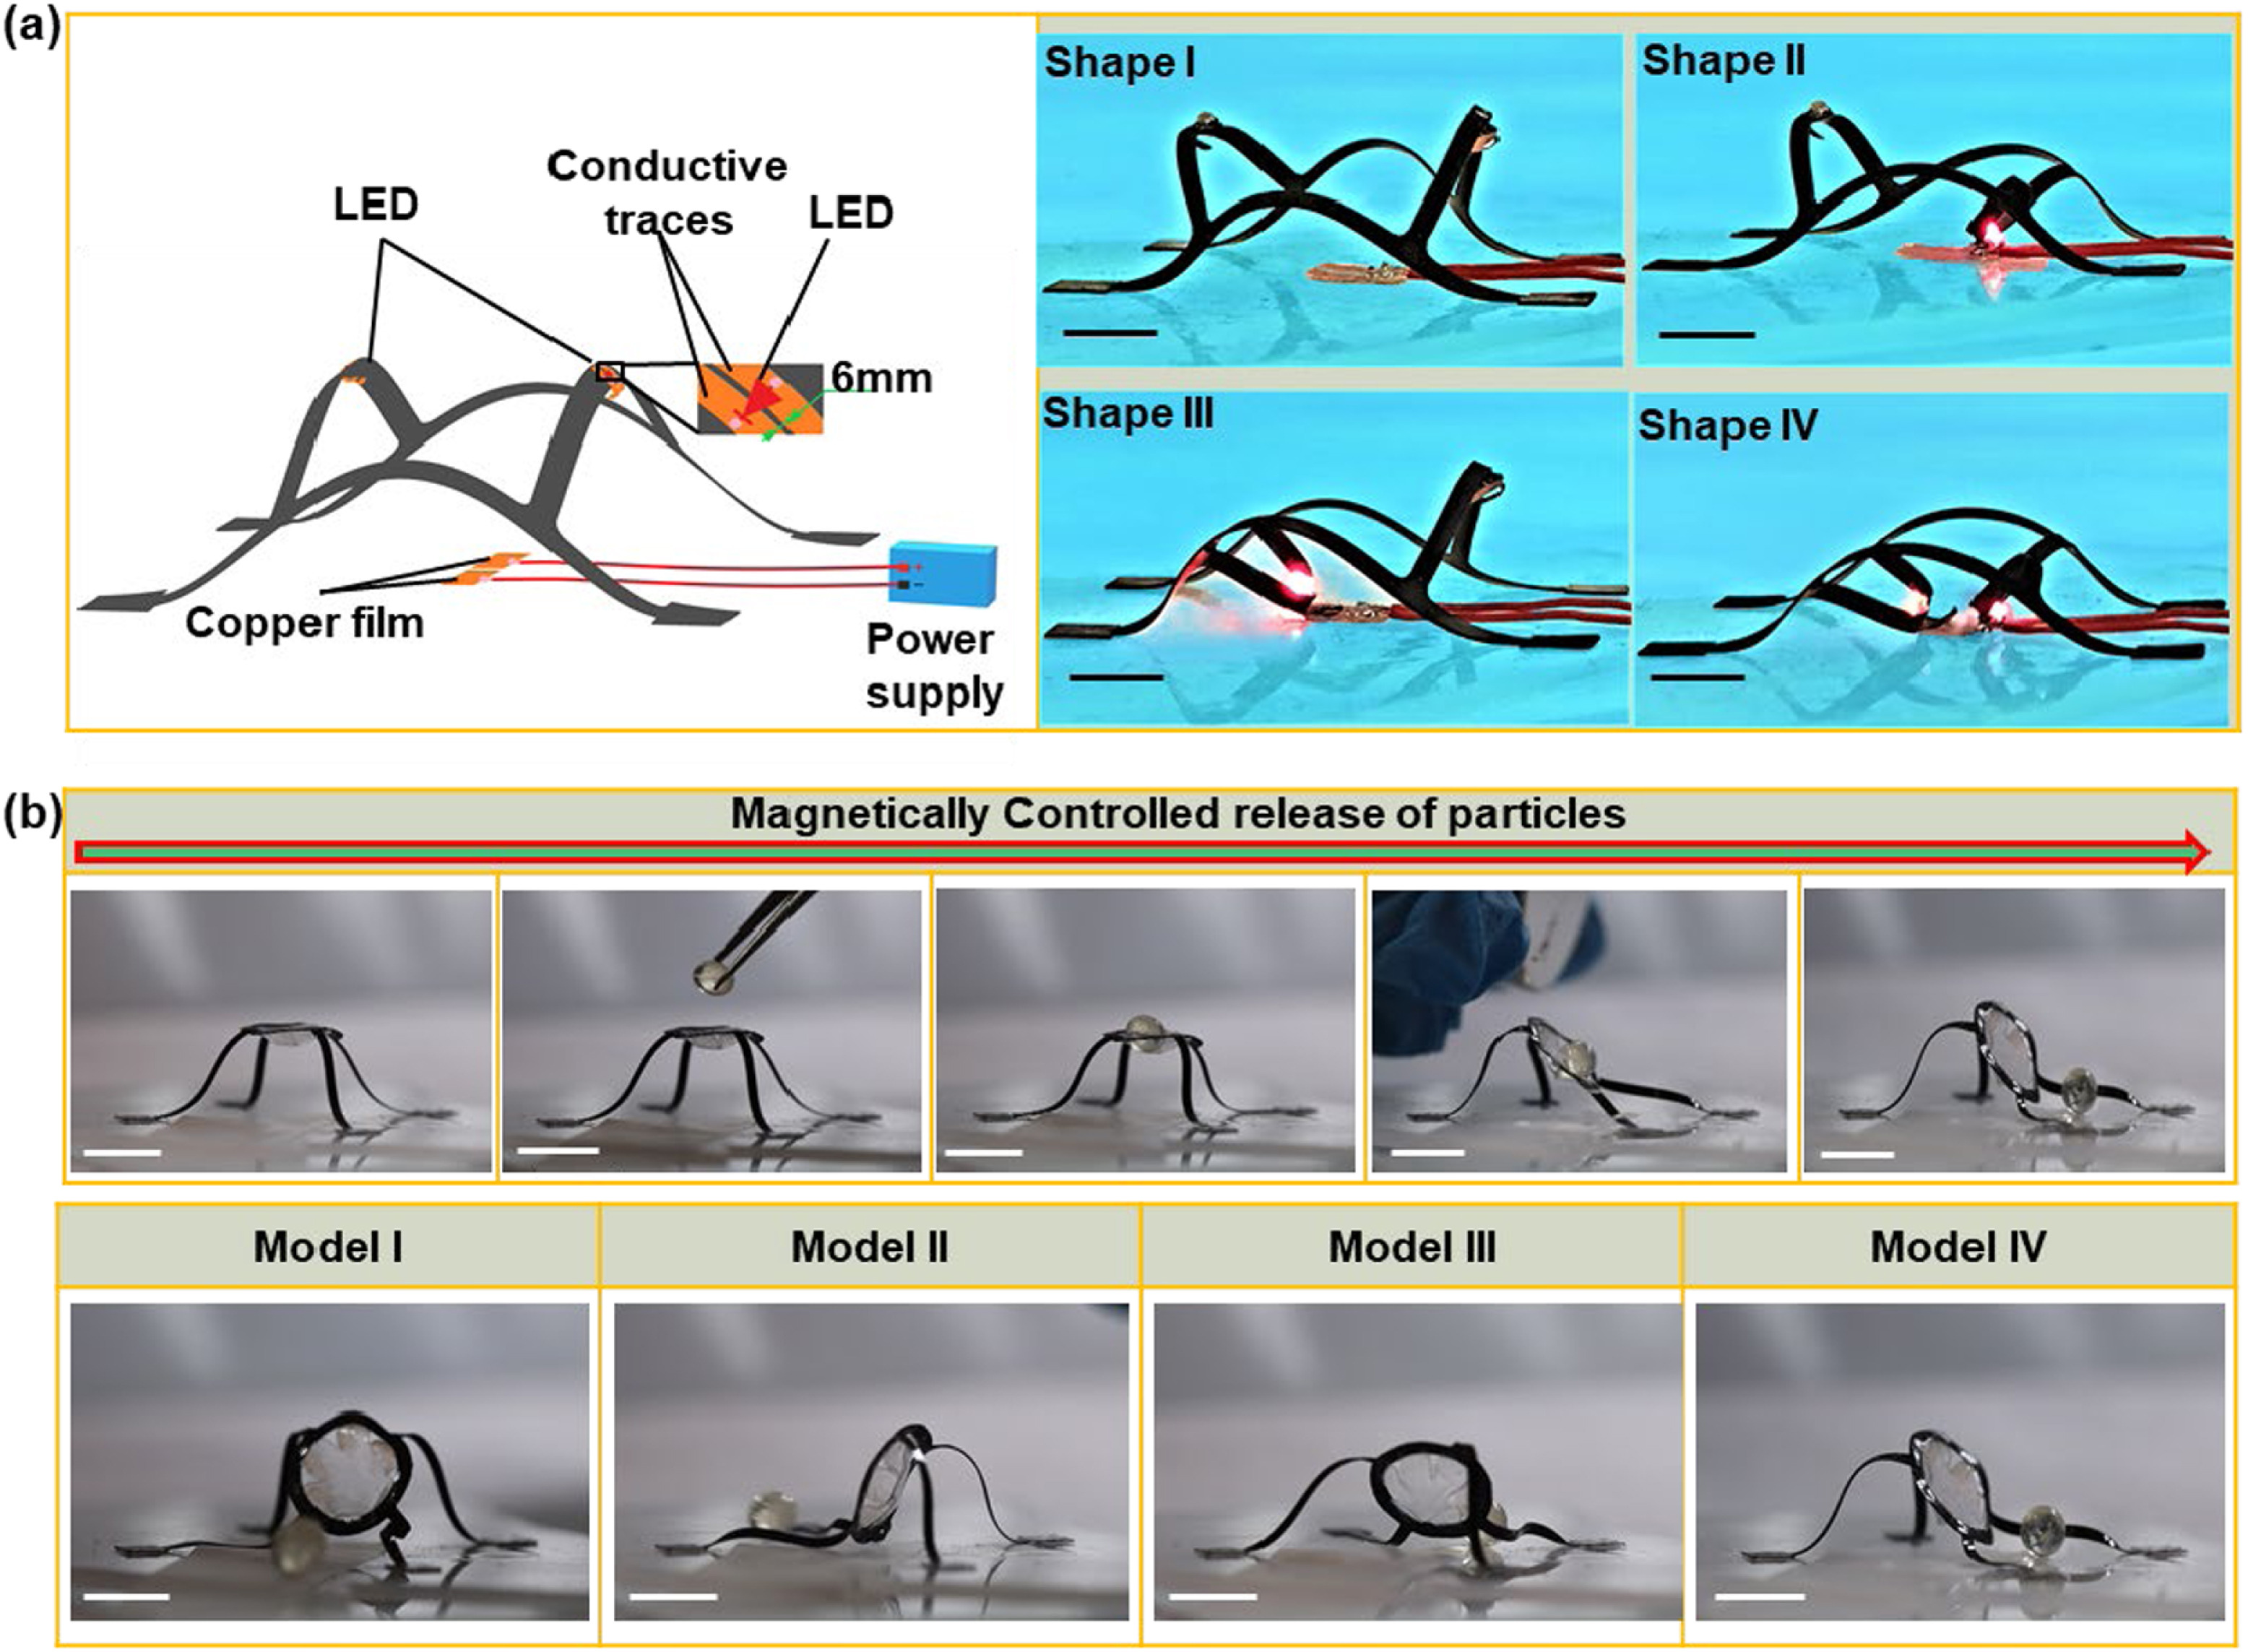
\includegraphics[width=\textwidth]{figure5.jpg}
  \caption{
    Applications of reconfigurable structures in on-demand 3D light emitting systems and controlled particle delivery.
    (a) Schematic illustration and optical images of a 3D light emitting system that can be reconfigured among its multistable states to switch the LEDs on and off.
    (b) Controlled release of particles in four different directions (Modes I-IV) enabled by four possible stable states of the table structure.
    Scale bars, \SI{1}{\centi\meter}.
  }
  \label{fig:ms-5}
\end{figure}

Based upon our investigations of the 3D table structure, a device is created for the delivery of particles in a well-controlled manner.
As shown in \cref{fig:ms-5}(b), a thin layer of pure PDMS film is placed in a concave shape in the centre of the table, in order to support a silica particle.
This film that supports the particle is insensitive to the applied magnetic field when the table structure is magnetically actuated, thereby exerting minimal influence on the reconfiguration of the whole structure.
The table structure itself is designed to be in the 2 state region of the phase diagram, \cref{fig:ms-1}(c), such that it exhibits one upright state and a second state in four different orientations (modes I-IV).
To trigger the delivery of the particle, a portable magnet is used to manipulate the structure into one of these different orientations, leading to well-controlled particle delivery in a chosen direction.
Therefore, such flexible, remotely reconfigurable structures could have a lot of potential applications in controlled delivery.



\section{Discussion}

To conclude, we have tightly integrated experiments and modelling to survey the energy landscapes of highly nonlinear 3D ferromagnetic structures for the development of reconfigurable systems.
Our systematic computational analysis predicts a design phase diagram for a targeted number of stable states by varying essential material properties and geometries.
It also allows us to systematically identify highly complex transition paths among the distinct stable states that minimise the energy barriers, without the need to prescribe an expected pathway for structural transformations a priori.
These predictions are thoroughly validated by our experiments of creating multistable 3D ferromagnetic structures and magnetically reconfiguring the structures among their multistable states following different pathways rapidly, in a remote, on-demand manner.

Using this strategy, a plethora of symmetric and asymmetric 3D mesostructures of diverse geometries are realised and reconfigured among their multistable states, including those that resemble ribbons, tables, baskets, flowers, boxes, single and double beams.
These versatile reconfigurable structures have a range of possible applications, illustrated by the integration of electronic components to create reconfigurable light-emitting functional devices, and a magnetically actuated table structure for particle delivery.

We believe our fundamental studies on the reconfigurational behaviours of 3D structures establish the foundations for a robust and reproducible modelling approach that may be applied more broadly to the design and development of diverse types of reconfigurable structures and systems.
This may include origami, kirigami and stimuli-responsive structures beyond magnetic actuation, where the exploration of energy landscapes could aid in understanding the reconfiguration and the tunability of multistable states.

It is also interesting to explore the integration of functional materials with locally patterned magnetic films of different magnetization directions \cite{Kim2018,Alapan2020}, and stiffness manipulation \cite{Zhai2020} to expand the design space of possible hybrid structures and to potentially enable multi-stimuli-responsive structures and soft machines.
We believe these studies will provide important insights for the design of reconfigurable structures and functional systems for wide-ranging applications, such as in deployable solar panels, phononics, morphable architected materials, and soft robotics.

\begin{table}[]
  \begin{tabularx}{\textwidth}{>{\hsize=.3\hsize\linewidth=\hsize}C >{\hsize=.55\hsize\linewidth=\hsize}C >{\hsize=2.1\hsize\linewidth=\hsize}C >{\hsize=1.05\hsize\linewidth=\hsize}C}
    \hline\hline
    Topic & Symbol & Parameter description & Value \\
    \hline
    \multirow{9}{*}{\rotatebox[origin=c]{90}{Structure}}
          & $L$            & Arm width              & 1.04 / 0.8 / \SI{0.5}{\milli\metre} \\
          & ---            & Arm length             & $12.5 L$ \\
          & $r_\text{out}$ & Outer ring radius      & $5 L$ \\
          & $r_\text{in}$  & Inner ring radius      & $3.75 L$ \\
          & ---            & Mesh resolution        & $0.1 L$ \\
          & $t$            & Thickness              & \SI{150}{\micro\metre} \\
          & $\rho$         & Density                & \SI{2.59}{\gram\per\centi\meter\cubed} \\
          & $Y$            & Young's modulus        & \SI{1.4}{\mega\pascal} \\
          & $\nu$          & Poisson ratio          & 0.3 \\
          & ---            & Compressive strain     & 0.3 \\
    \hline
    \multirow{4}{*}{\rotatebox[origin=c]{90}{L-BFGS}}
          & $m$      & Iteration memory             & 10 \\
          & ---      & Initialisation iterations    & \num{10000} \\
          & ---      & Initialisation force density & \SI{10}{\newton\per\meter\squared} \\
          & ---      & Gradient RMS convergence     & $10^{-10}$ \\
    \hline
    \multirow{6}{*}{\rotatebox[origin=c]{90}{Pathways}}
          & $\alpha$ & BITSS energy constraint strength    & 10 \\
          & $\beta$  & BITSS distance constraint error     & 0.1 \\
          & $f$      & BITSS distance reduction factor     & 0.5 \\    
          & ---      & BITSS coefficient regularity        & 100 iterations \\    
          & ---      & String reparametrisation regularity & 300 iterations \\
          & ---      & String number of images             & 20 \\
    \hline\hline
  \end{tabularx}
  \caption{\label{tab:ms-params}
    Values of the parameters that are used throughout this chapter, unless otherwise specified.
  }
\end{table}

  \chapter{Origami-inspired Mesostructures}
\label{ch:origami_ribbon}
\graphicspath{{origami_ribbon/fig/}}

This chapter is based upon the joint work: Y. Li, S. J. Avis, T. Zhang, H. Kusumaatmaja, and X. Wang, ``Tailoring the multistability of origami-inspired, buckled magnetic structures via compression and creasing'', \emph{Mater. Horiz.}, 8, 3324 (2021).

In particular, the experimental ferromagnetic structures are the work of Y. Li, while the simulations and energy landscape analysis are my own work.



\section{Introduction}

Origami, the ancient art of folding two-dimensional (2D) thin sheets along predefined creases to create three-dimensional (3D) objects\cite{Chen2015,Dudte2016,Ning2018}, has inspired the design of many engineering structures for a wide range of applications, including deployable systems\cite{Thesiya2015,Melancon2021,Liu2020}, self-folding machines\cite{Felton2014}, reconfigurable metamaterials\cite{Silverberg2014,Chen2021,Yang2019}, and DNA origami\cite{Hellmeier2021}.
For those applications, a key design feature of the structures is their ability to have multiple stable states as well as the tailoring of those states for tunability and adaptability.
Existing works so far have primarily focused on bistable systems for rigid origami patterns (like the Miura folding\cite{Miura1985} and its derivatives\cite{Filipov2015}) and deformable origami (like the twisted square pattern\cite{Silverberg2015}).
For example, Sadeghi and Li realised rapid and reversible folding by harnessing the asymmetric bistability of designed origami structures\cite{Sadeghi2020}.
Liu et al. demonstrated that a folded hypar origami, obtained by folding a piece of paper along concentric squares and their diagonals to arrive at a seemingly smooth saddle shape, exhibits bistability between two symmetric configurations\cite{Liu2019b}.
More recently, Melancon et al. realised pressure-deployable origami structures characterised by two stable configurations — one compact and one expanded – at the meter scale\cite{Melancon2021}.
Furthermore, Fang et al. showed that the potential energy landscapes of stacked Miura-ori and the Kresling-ori structures, and therefore their stability profiles and constitutive force–displacement relations, can be effectively tuned by embedded magnets\cite{Fang2019}.

In addition to multistability, reconfiguration among the different stable states of origami-inspired structures in a well-controlled manner is demanded in many engineering devices and structures.
Theoretical and experimental studies have been performed on reconfiguration paths in origami-inspired structures.
For example,  Zhai et al. created an origami-inspired mechanical metamaterial that can be deployed and collapsed along different configuration paths\cite{Zhai2018}.
Silverberg et al. showed that hidden degrees of freedom in square twist origami structures give rise to a critical transition from mono- to bi-stability\cite{Silverberg2015}.
Moreover, significant advances have been made to improve the tunability and adaptability of origami-inspired structures by incorporating stimuli-responsive materials, which provides opportunities for micro robotics, biomedical devices, and many others\cite{Jamal2013,Chen2020,Xu2017,Novelino2020,Xu2017a}.

Previous studies have laid solid foundations for the design and development of origami-inspired structures with bistability and tunability.
One of the remaining challenges in this field is to actively control the number of possible stable states and their reconfiguration paths.
Here we investigate this by extending our studies of mesostructures from the previous chapter to incorporate origami-inspired creases, which can increase the prevalence of multistable states.
There are innumerable structures that can be constructed from networks of creased ribbons, so we instead restrict our attention to the most simple structure, a single ribbon with multiple creases, to gain fundamental insights about the effect of creases on multistability.
However, the same approaches could also be applied to study other structures.

The two key parameters that we control are compressive strain and creasing in the ribbon, which are selected because they are easy to tune and very effective to alter the multistable behaviors of the structure for real applications.
We utilise a similar computational approach as the last chapter in order to construct phase diagrams showing how the available states sensitively depend on the compressive strain and the number of creases.
Then we generate the the reconfiguration pathways to understand the stability of the various states and how they can interchange upon applying an external magnetic force or varying the applied strain.

Finally, guided by this analysis, our collaborators have produced diverse complex origami-inspired structures, including structure arrays that be individually tuned based on the multistability of the structural unit and a biomimetic insect.



\section{Results and Discussion}

\subsection{Concept of origami-inspired, multistable magnetic structures}

\Cref{fig:or-1} schematically illustrates the experimental assembly process and reconfiguration of origami-inspired structures compressively buckled from ferromagnetic composites\cite{Wang2019a,Zhang2015,Liu2019}.
These are constructed using the approach described in \cref{ch:mesostructures}, however laser patterning is also used in order to create crease sections with a thickness that is 46.15\% of the non-crease regions.
Due to this reduced thickness, the crease regions act as flexible hinges that can bend into different states, affecting the potential multistable reconfigurations\cite{Tang2019}.

Under an external magnetic field generated by a manually manipulative magnet, the assembled origami-inspired structure can be reconfigured into up to four distinct stable states: state 1 (S1, one center peak), state 2 (S2, one side peak), state 3 (S3, two peaks), and state 4 (S4, twisted two peaks).
These are then able to remain stable after the removal of the applied magnetic field.

\begin{figure}
  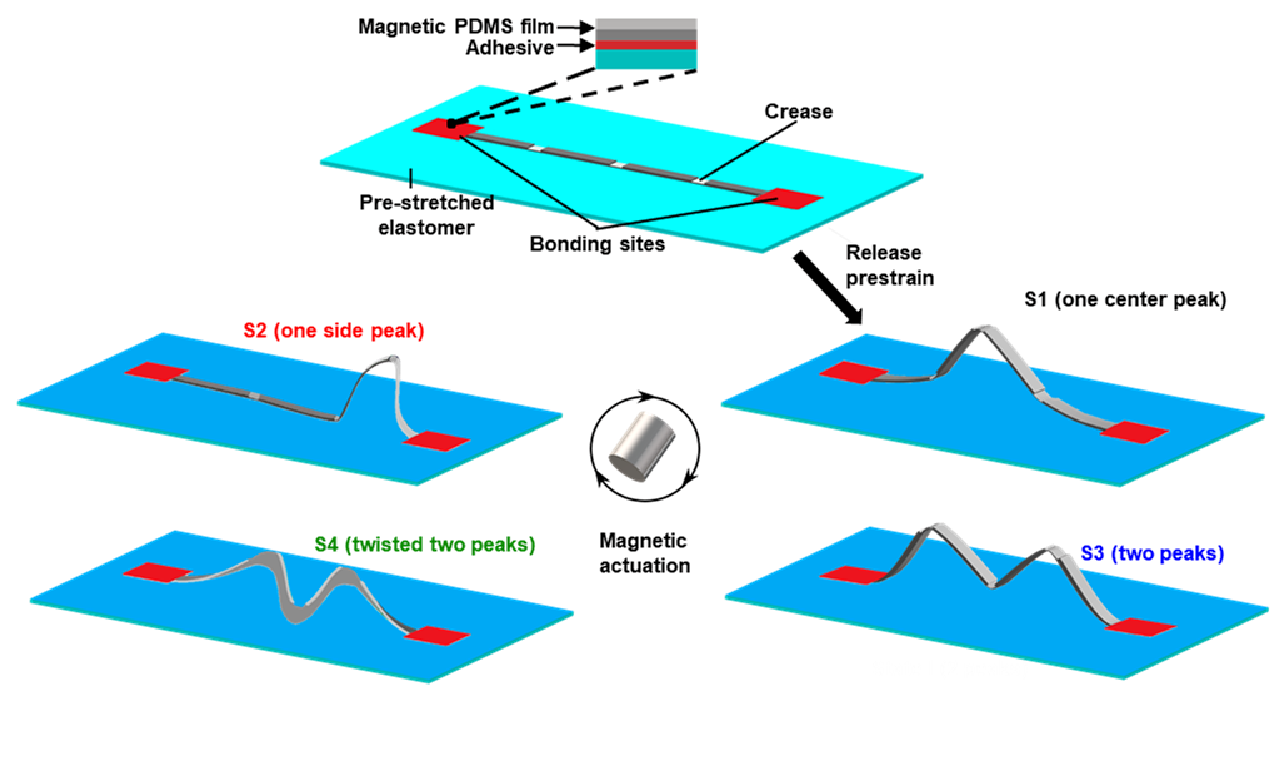
\includegraphics[width=\textwidth]{figure_1.pdf}
  \caption{
    Schematic illustration of the assembly and magnetic reconfiguration schemes of multistable origami-inspired ribbon structures.
  }
  \label{fig:or-1}
\end{figure}


\subsection{Phase diagram of stable states for origami-inspired structures}

We first study the effect of two essential parameters, the number of creases and compressive strains, on the number and configurations of stable states by using a ribbon structure as an example.
A phase diagram, indicating the stable states of the structure with up to seven creases and at strain levels of 0\%-40\%, is shown in \cref{fig:or-2}(a) and serves as a theoretical foundation for the multistability design.
The phase diagram is constructed computationally by identifying the local minima in the energy landscape of the structure under various conditions of strain levels and crease numbers.

As in \cref{ch:mesostructures}, we have used the discrete shell model, this time with two thicknesses: \SI{130}{\micro\meter} and \SI{60}{\micro\meter}, combined with a random search algorithm for energy minimisation.
At selected points (typically 5 different strain levels for each crease number) across the phase diagram, the structure is randomly initialised several hundreds of times and relaxed to the minima.
Once the qualitatively distinct configurations are identified, we systematically vary the compressive strain to observe the full range over which each state is stable.
It is worth noting that while it is difficult to guarantee that all possible stable states have been obtained, we are unable to find additional states when more points in the phase diagram are sampled.
Hence, we consider the identified stable states to be representative in this study.

\begin{figure}
  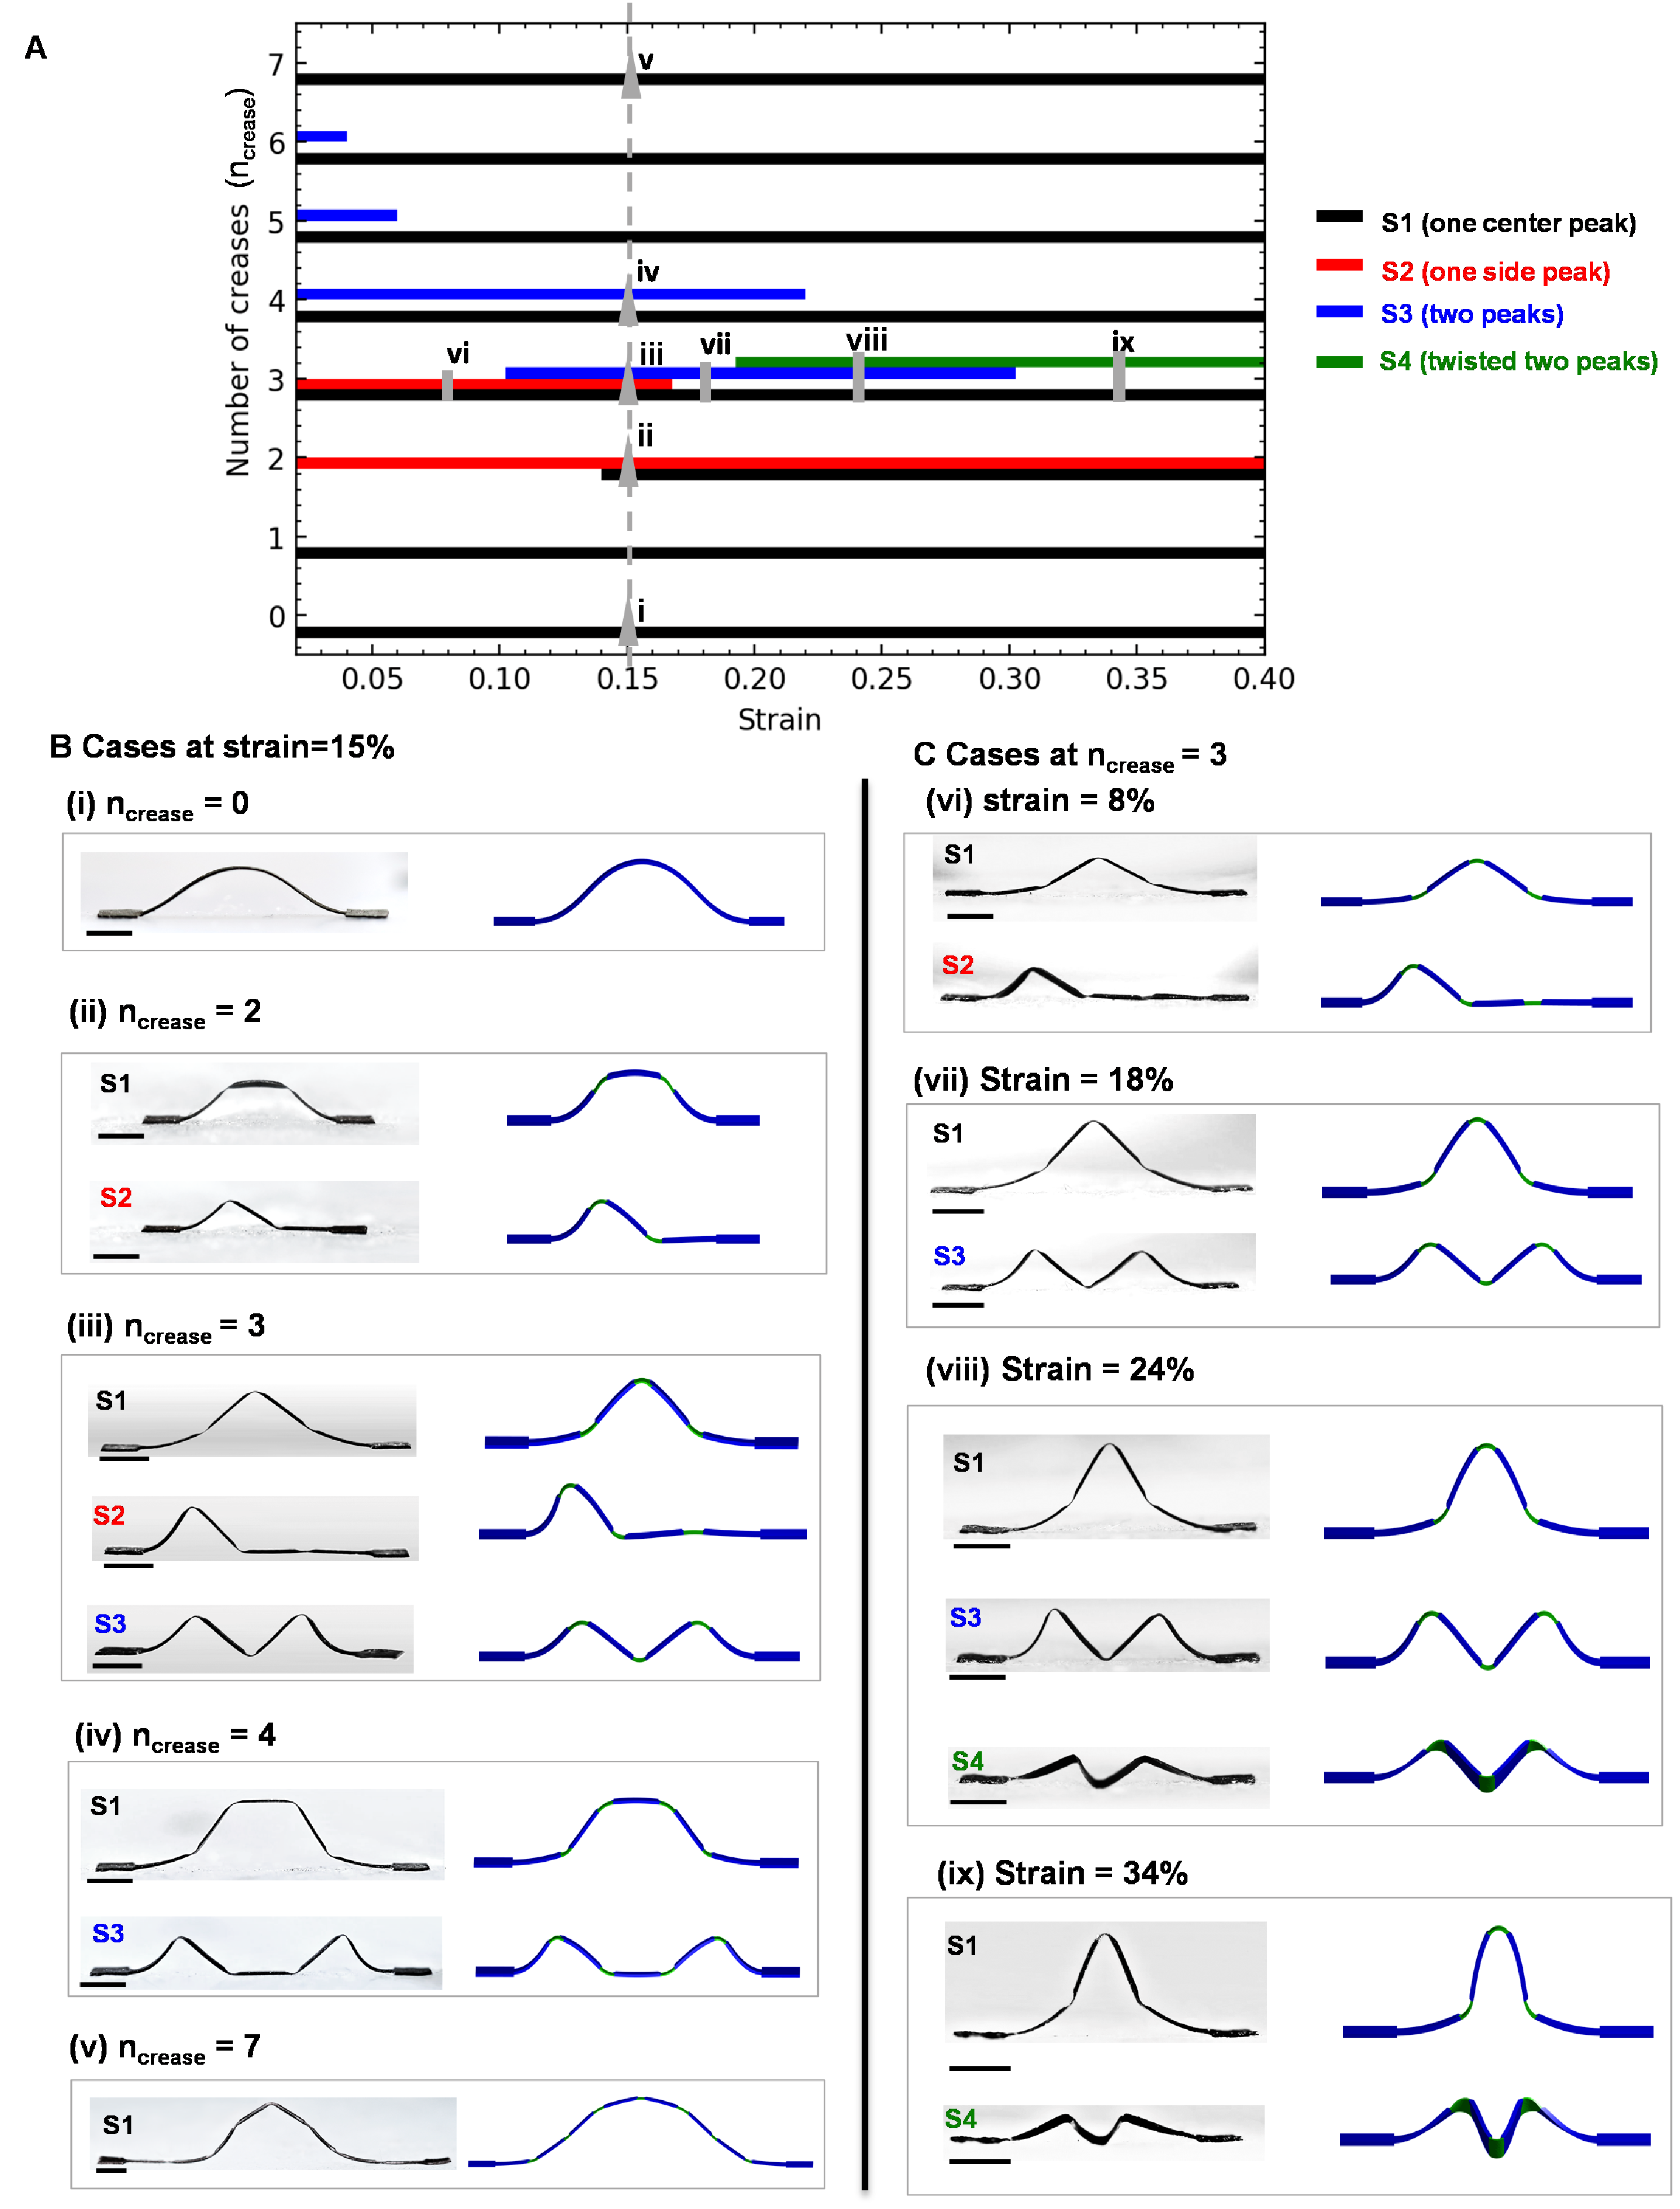
\includegraphics[width=\textwidth]{figure_2.pdf}
  \caption{
    Multistability of origami-inspired ferromagnetic ribbon structures under varying creases and compressive strains.
    (A) Design phase diagram showing the effect of the crease number and compressive strain on the number and configurations of distinct stable states of the ribbon.
    (B) Experimental and computational results of multistable states under a constant strain of 15\% and varying crease numbers, corresponding to points i-v labelled in \cref{fig:or-2}(a).
    Scale bars, 2 mm.
    and (C) Experimental and computational results of multistable states at a constant number of creases ($n_\text{crease} = 3$) and varying strain levels, corresponding to points vi-ix in \cref{fig:or-2}(a).
    Scale bars, 2 mm.
  }
  \label{fig:or-2}
\end{figure}

As shown in \cref{fig:or-2}(a), the number of creases ($n_\text{crease}$) has notable effects on the number and configurations of stable states.
To better illustrate this point, we demonstrate the available states of structures as $n_\text{crease}$ is increased from 0 to 7 under a constant compressive strain of 15\% in \cref{fig:or-2}(b), with the computational and experimental results shown side by side.
When the $n_\text{crease}$ is zero, i.e., the continuous ribbon structure, only S1 (one center peak) exists at all strain levels (e.g., point i).
An additional asymmetric state S2 becomes available when $n_\text{crease}$ rises to two at a compressive strain of 15\% (point ii).
A further increase to three creases causes the structure to admit state S3 (two peaks) at a strain of 15\% (point iii) and S4 (twisted two peaks) at a higher strain level.
As $n_\text{crease}$ increases above three, the number of stable states begins to decline, with S2 becoming unstable for structures with four creases (point iv).
For structures with five creases and above, only S1 remains stable at a compressive strain of 15\%, although S3 is still stable under lower strains for $n_\text{crease}=5$ and 6.
This can be expected because we are approaching the continuous case when the number of creases is large.

The available stable states also depend strongly on the magnitude of the applied compressive strain used in the assembly process of the structure.
We illustrate this using a structure with three creases due to its rich phenomena.

Based on the number and configurations of stable states, five regimes are identified: a) two distinct stable states (S1 and S2; 0-10\% strain), b) three distinct stable states (S1, S2, and S3; 10-17\% strain), c) two distinct stable states (S1 and S3; 17-19\% strain), d) three distinct stable states (S1, S3, and S4; 19-30\% strain), and e) two distinct stable states (S1 and S4; 30-40\% strain).
\Cref{fig:or-2}(c) shows experimental and computational results of distinct stable states at representative strain levels for the five regimes.
Under a relatively low compressive strain of 8\% (point vi), states S1 (one center peak) and S2 (one side peak) exist, which can be reversibly reconfigured into each other via manually controlling the magnetic force and direction.
Increasing the strain to 15\% (point iii) leads to the appearance of a third state, S3 with two peaks, which increases the number of stable states to three.
However, when the strain is further increased to 18\% (point vii), S2 with one side peak disappears.
Further increasing the strain to 24\% (point viii) causes the formation of an interesting twisted state (S4) and therefore increases the number of stable states to three (S1, S3 and S4).
As the strain becomes even larger, S3 disappears and only S1 and S4 exist at the strain of 34\% (point ix).

The experimental and computational results shown above agree reasonably well.
The discrepancy in the configuration of some stable states (e.g., (v) S1 in \cref{fig:or-2}(b)) between experiments and modeling likely results from the adhesion and friction between the structure and the substrate in experiments, which is neglected in computational modeling.
The effect of friction will be further discussed in \cref{sec:or-paths}.

Furthermore, by continuously changing the strain levels from 0\% to 40\% using the 3-crease structure, we record the dynamic progression of the five regimes and the fast, remote magnetic reconfiguration among the stable states within each regime in \cref{vid:ribbon-progress}, which is highly consistent with the predictions of the phase diagram in \cref{fig:or-2}(a).
We also show that the states are stable under perturbations perpendicular to the vertical surface (along the height direction) of the ribbon, except in cases where S4 (twisted two peaks) is present.

The studies above provide important guidelines for tailoring the number and configurations of stable states in origami-inspired structures by tuning the number of creases and the assembly strain.
For example, for applications like digital logics where multiple stable states are desired, structures with three creases may offer more design space and tunability, while structures with a lower or higher number of creases is preferred for applications where a single stable state is needed.

Furthermore, from the phase diagram, we observe that structures with two and three creases have multistable states under a wide range of strain (15\%-40\% strain for the case of two creases and 0\%-40\% strain for the case of three creases), which can be used for applications of multistable structures that demand a wide working strain range.

\subsubsection{Effect of crease thickness and length}
As a brief aside, we also study the effects of modifying the crease thickness ratio and length ratio (defined with respect to the length of each flat segment) on the multistability.
For this, the 3-crease ribbon under a strain level of 14\% is used as an example.

\begin{table}[htb]
  \setkeys{Gin}{width=\linewidth}
  \begin{tabularx}{\textwidth}{CCCCC}
    \hline\hline
    Thickness ratio & State 1 & State 2 & State 3 & State 4 \\
    \hline
    0.67 & 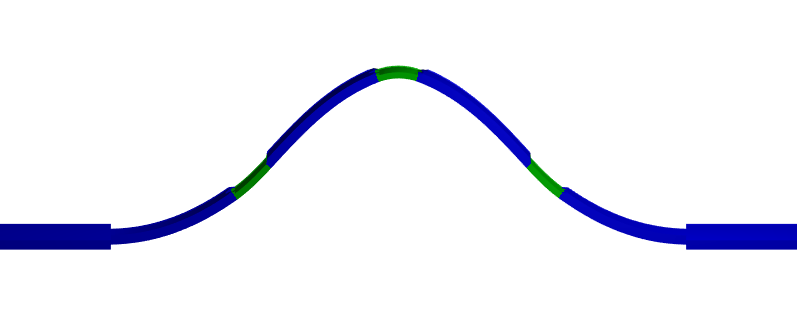
\includegraphics{tratio/1-0.67.png} & \xmark                              & \xmark                          & \xmark \\
    0.56 & 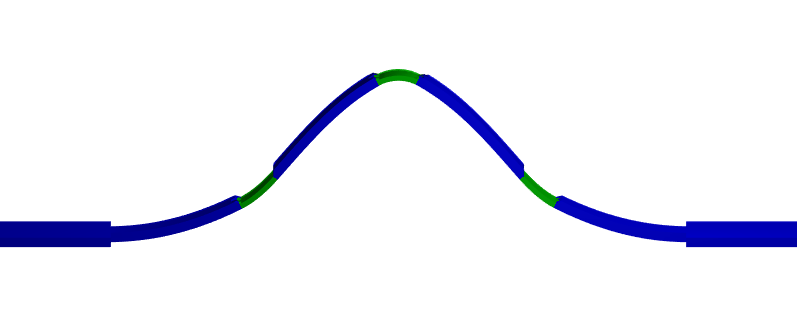
\includegraphics{tratio/1-0.56.png} & 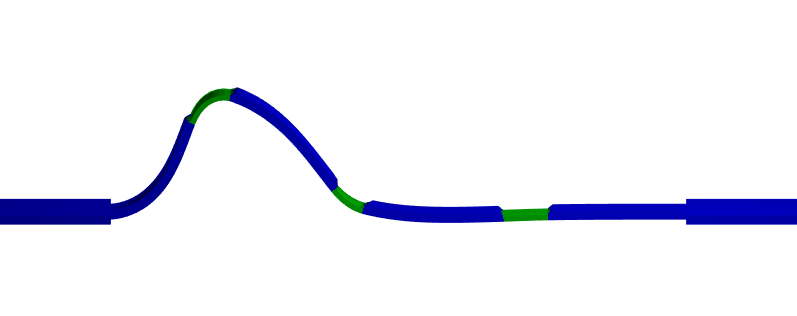
\includegraphics{tratio/2-0.56.png} & \xmark                          & \xmark \\
    0.46 & 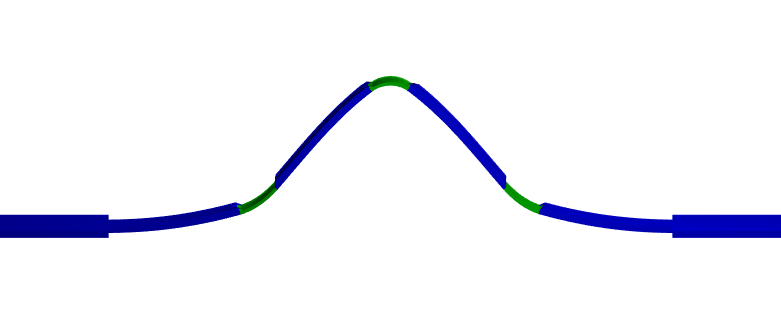
\includegraphics{tratio/1-0.46.png} & 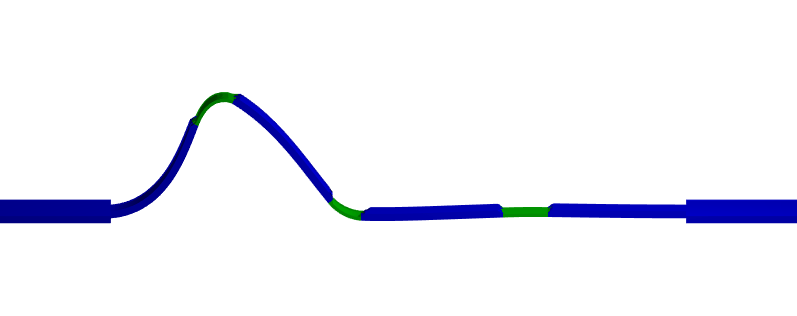
\includegraphics{tratio/2-0.46.png} & 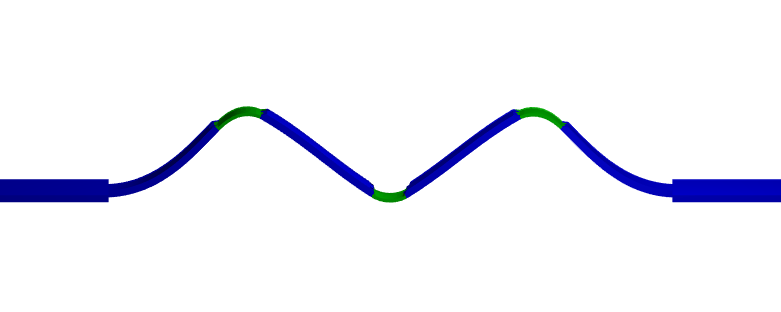
\includegraphics{tratio/3-0.46} & \xmark \\
    0.33 & 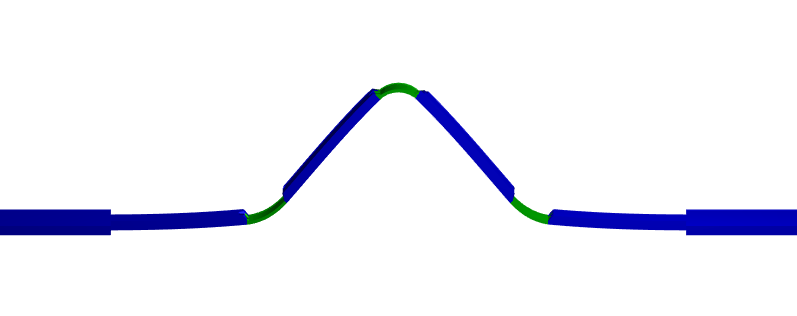
\includegraphics{tratio/1-0.33.png} & \xmark                              & 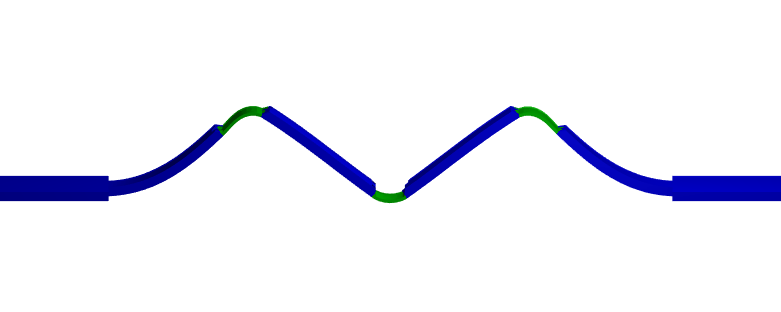
\includegraphics{tratio/3-0.33} & 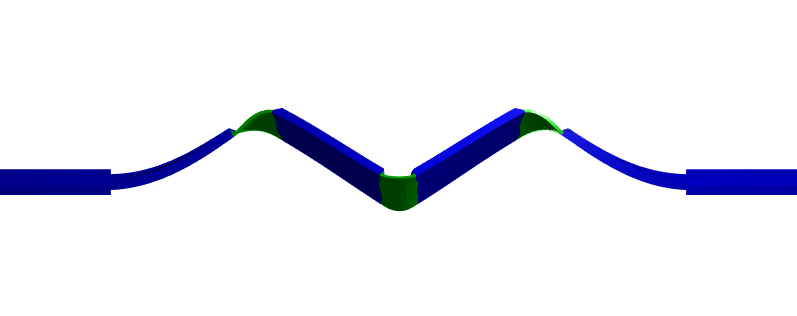
\includegraphics{tratio/4-0.33.png} \\
    0.25 & 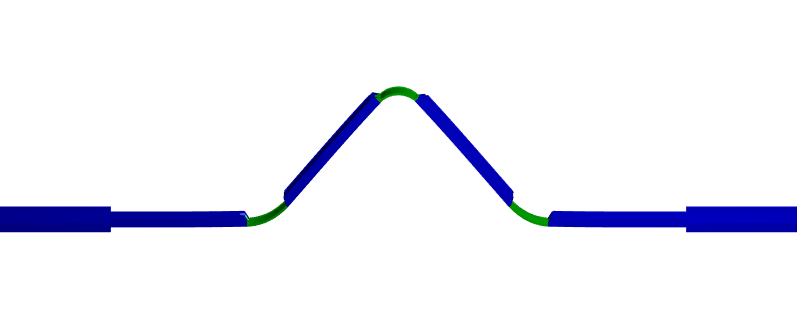
\includegraphics{tratio/1-0.25.png} & \xmark                              & 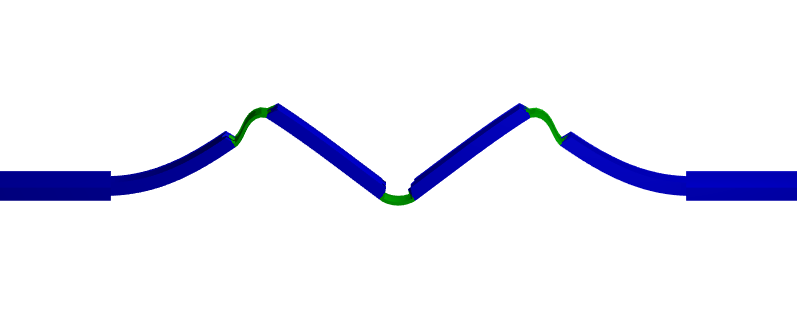
\includegraphics{tratio/3-0.25} & \xmark \\
    \hline
  \end{tabularx}
  \caption{Effect of the crease thickness ratio on the multistability of the ribbon structure (strain: 14\%; length ratio: 0.32)}
  \label{tab:or-S1}
\end{table}

\begin{table}[htb]
  \setkeys{Gin}{width=\linewidth}
  \begin{tabularx}{\textwidth}{CCCCC}
    \hline\hline
    Length ratio & State 1 & State 2 & State 3 & State 4 \\
    \hline
    0.10 & 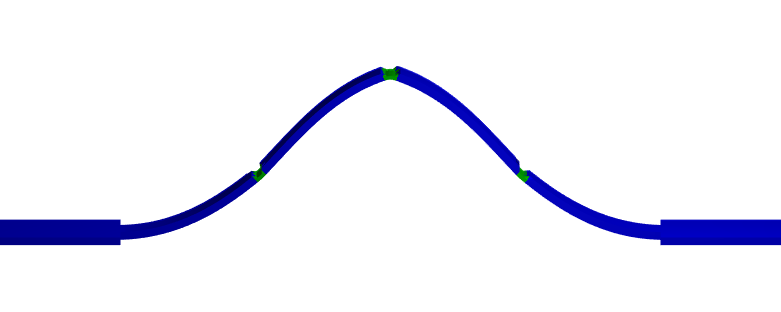
\includegraphics{lratio/1-0.1.png}  & \xmark                              & \xmark                          & \xmark \\
    0.18 & 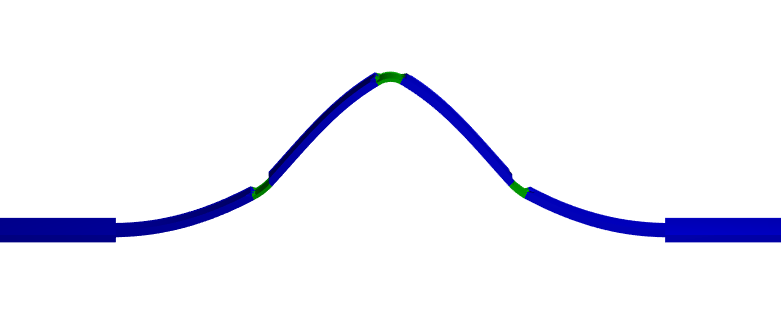
\includegraphics{lratio/1-0.18.png} & 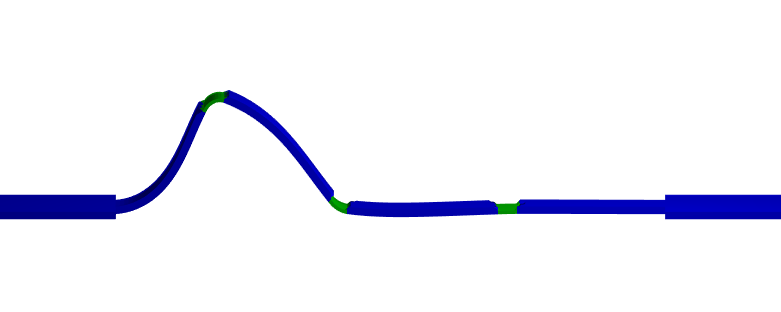
\includegraphics{lratio/2-0.18.png} & \xmark                          & \xmark \\
    0.32 & 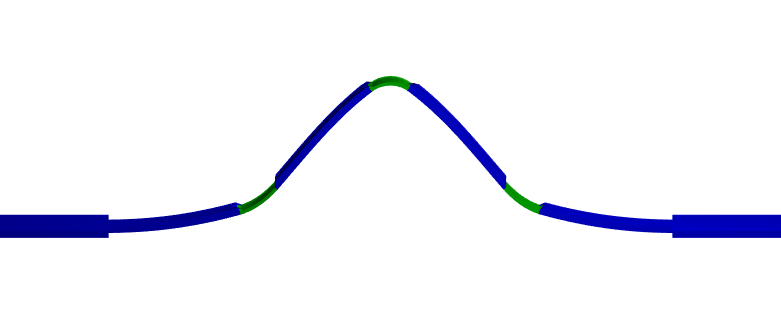
\includegraphics{lratio/1-0.32.png} & 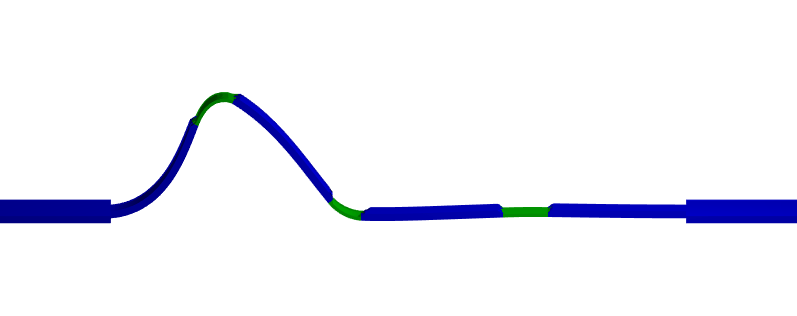
\includegraphics{lratio/2-0.32.png} & 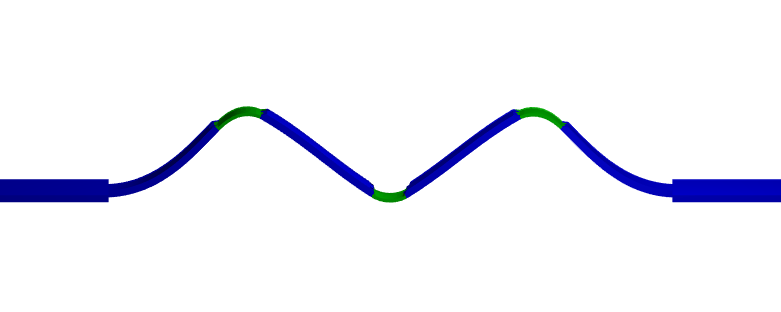
\includegraphics{lratio/3-0.32} & \xmark \\
    0.56 & 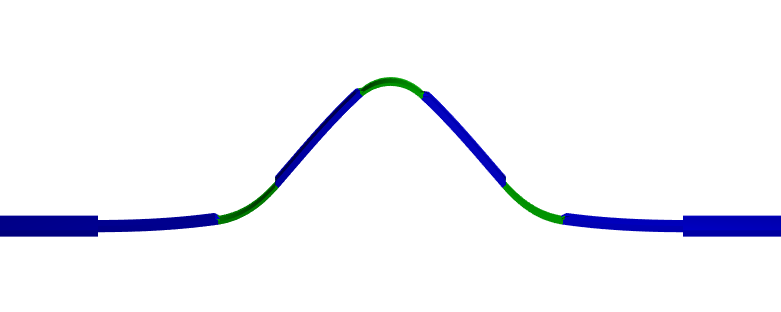
\includegraphics{lratio/1-0.56.png} & 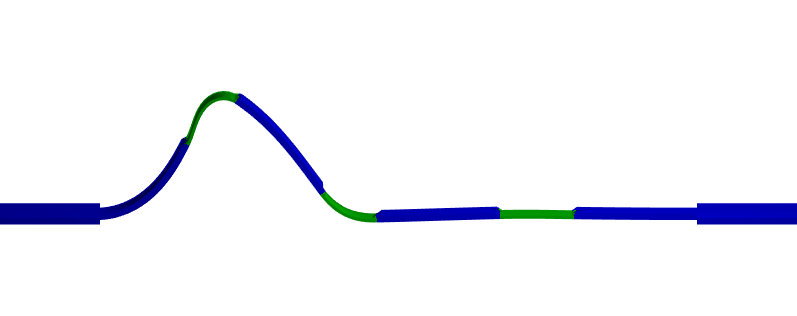
\includegraphics{lratio/2-0.56.png} & 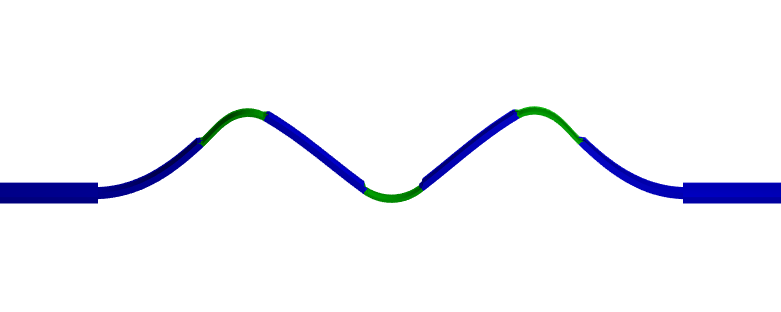
\includegraphics{lratio/3-0.56} & 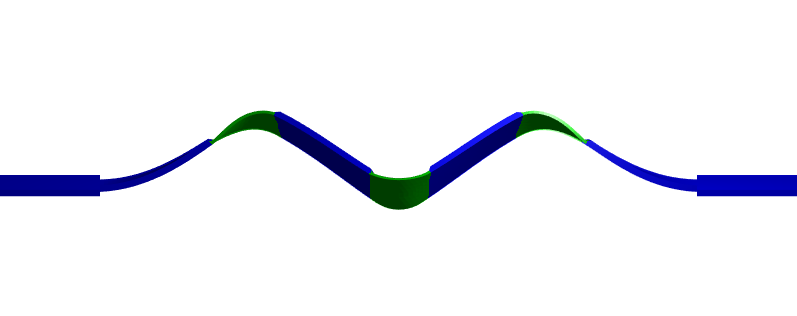
\includegraphics{lratio/4-0.56.png} \\
    1.00 & 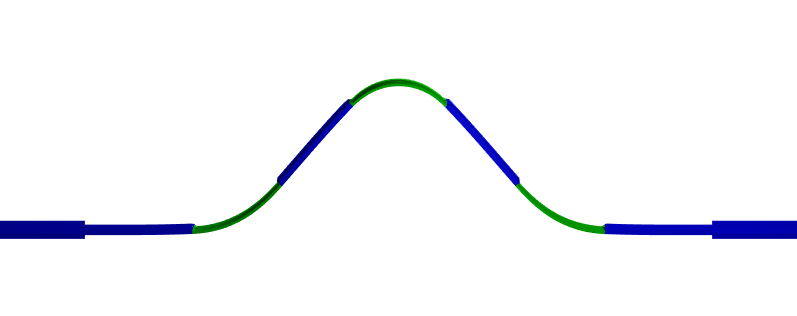
\includegraphics{lratio/1-1.png}    & \xmark                              & 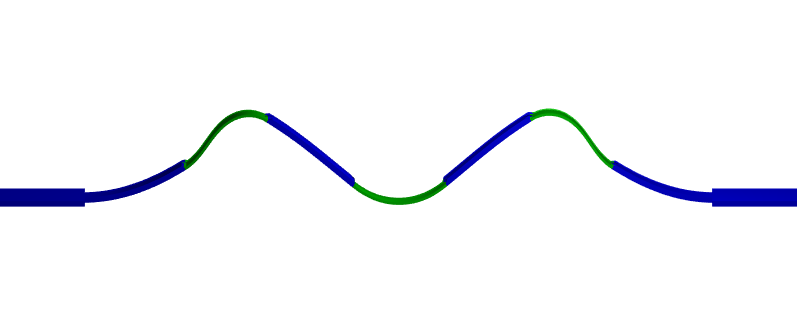
\includegraphics{lratio/3-1}  & 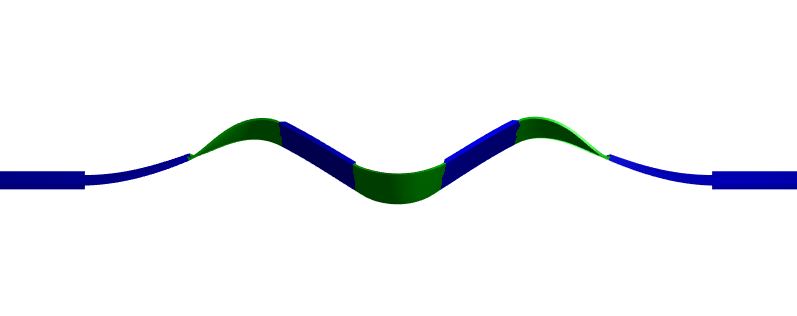
\includegraphics{lratio/4-1.png} \\
    \hline
  \end{tabularx}
  \caption{Effect of the crease length ratio on the multistability of the ribbon structure (strain: 14\%; thickness ratio: 0.46)}
  \label{tab:or-S2}
\end{table}

The results in \cref{tab:or-S1,tab:or-S2} show that both ratios can have a significant effect on the multistability of the ribbon structure.
In particular, reducing the crease thickness and increasing its length has an overall similar effect on the stable states as increasing the compressive strain.
The main difference is at the extreme when state 3 remains stable, rather than progressing to the twisted state.
This is because reducing the thickness of the crease, or increasing its length, grants the creases more flexibility, which reduces the amount of bending that is required in the edge segments.
However, it is likely that at larger compressive strains state 3 will become unstable.


\subsection{Reconfiguration pathways for a 3-crease ribbon structure} \label{sec:or-paths}

In addition to locating the stable configurations, we also investigate available pathways that the structure can be reconfigured among its stable states, which is important for many applications.
The pathways have been computed using the same method as \cref{ch:mesostructures}, first by finding the TS with BITSS, for which the separation of the two states is reduced by 30\% each iteration, and then computing the pathways using a combination of downhill minimisation and the string method.
In addition, once a transition state is found for a given strain, a continuation approach is then used with the BITSS method in order to identify the energy barriers across the whole range of strains that the pathway exists.

\begin{figure}
  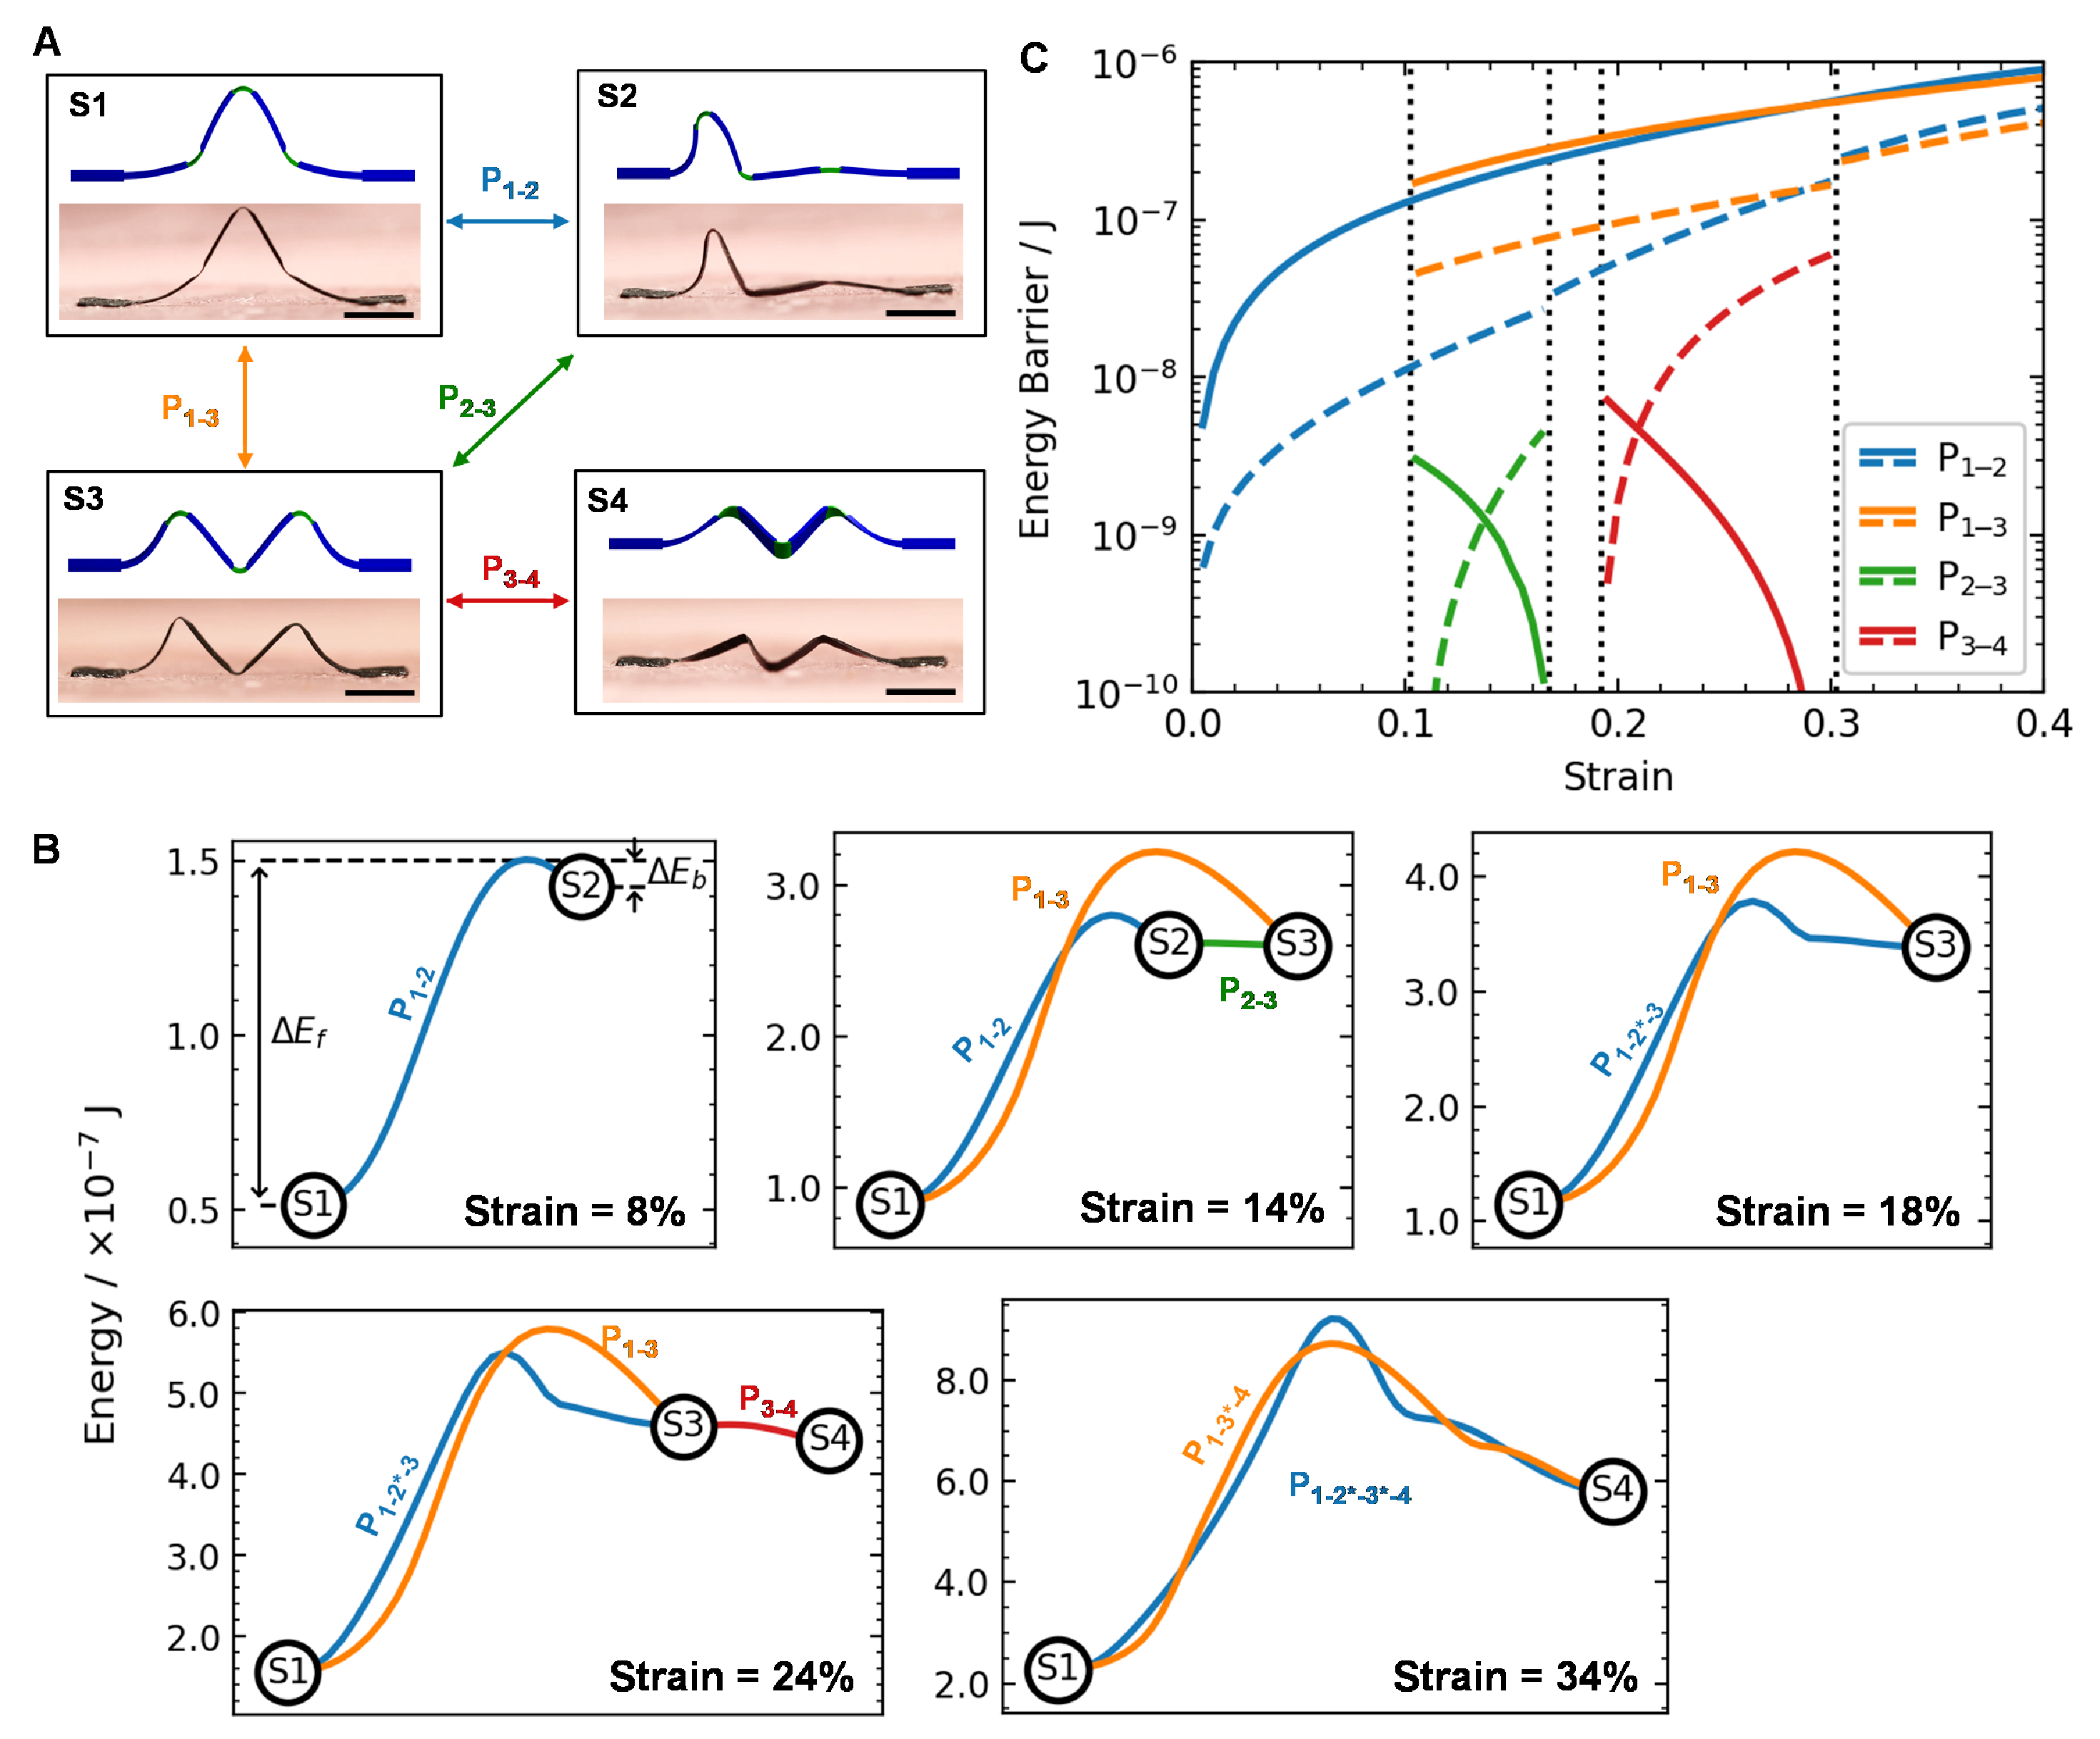
\includegraphics[width=\textwidth]{figure_3.pdf}
  \caption{
    (A) Reconfiguration paths among the distinct stable states of origami-inspired ferromagnetic ribbon structures.
    Scale bars, 2 mm.
    (B) Energy profiles of pathways for the 3-crease ribbon structure at various strain levels. (C) Minimum energy barriers for pathways in \cref{fig:or-2}(b) as a function of the strain.
    The solid lines indicate the energy barriers from the lower numbered states to the higher numbered states  and the dashed lines are the barriers from the higher numbered states to the lowered numbered states (illustrated by $\upDelta E_f$ and $\upDelta E_b$ in \cref{fig:or-3}(b), respectively) .
    The line colors correspond those in \cref{fig:or-3}(a).
    The blue and orange lines also encompass the extended pathways P\textsubscript{1-2*-3}, P\textsubscript{1-2*-3*-4}, and P\textsubscript{1-3*-4}.
  }
  \label{fig:or-3}
\end{figure}

Here we use the three-crease structure as a representative case for study because of its complexity in the configurations and the number of stable states, which results in a large number of reconfiguration paths.
As illustrated in \cref{fig:or-3}(a), we identify four distinct pathways among the stable states of the structure: P\textsubscript{1-2} for the transition path between S1 and S2, P\textsubscript{1-3} between S1 and S3, P\textsubscript{2-3} between S2 and S3, and P\textsubscript{3-4} between S3 and S4.
It is worth noting that in cases where one or more of those states are not stable, the corresponding individual paths may merge into one, as we will detail below.

\Cref{fig:or-3}(b) shows the available pathways and the associated energy profiles for a representative case in each of the five regimes for a 3-crease ribbon (identified in \cref{fig:or-2}(a)) as the strain is increased from 0\% to 40\%.
In the first regime (0-10\% strain), only states S1 and S2 exist, with a single pathway (P\textsubscript{1-2}) to reconfigure between them, as shown in \cref{vid:ribbon8}.
In the second regime (10\%-17\% strain), state S3 appears, so two additional pathways, P\textsubscript{1-3} and P\textsubscript{2-3}, become accessible (\cref{vid:ribbon14}).

Our analysis also highlights that there are not only multiple stable states existing in the structure, but also multiple available paths for transforming the structure from one state to another.
For example, we can observe that there are two main pathways that can be taken from state S1 to S3.
The first path, initially following P\textsubscript{1-2} to reconfigure S1 to S2, subsequently involves the creation of an asymmetric peak at one side of the structure to form state S3 from S2 (P\textsubscript{2-3}).
Due to symmetry, there are two equivalent scenarios depending on which side the peak is created to form S3.
The second path, P\textsubscript{1-3}, directly reconfigures S1 to S3 by forming two edge peaks simultaneously while maintaining symmetry.

As the strain increases to the regime of 17\%-19\%, state S2 becomes unstable, so P\textsubscript{1-2} and P\textsubscript{2-3} merge into a single path P\textsubscript{1-2*-3} (\cref{vid:ribbon18}), where 2* denotes that state 2 is no longer stable.
Above the strain of 19\%, pathway P\textsubscript{3-4} appears between state S3 and twisted state S4, while the two pathways from S1 to S3 still exist (\cref{vid:ribbon24}).
Finally, at the strain of 30\% and above, S3 is no longer stable leaving just two merged paths P\textsubscript{1-2*-3*-4} and P\textsubscript{1-3*-4} between S1 and S4 (\cref{vid:ribbon34}).

We further investigate the energy barriers of each pathway as a function of strain.
For each pathway, there are two relevant energy barriers, as illustrated in \cref{fig:or-3}(b) using P\textsubscript{1-2} in the case of 8\% strain as an example.
We label $\upDelta E_f$  for the energy required to transition from a lowered numbered state to a higher numbered state in each pathway (here, S1 to S2), while $\upDelta E_b$ is the energy required for the opposite transition (here, S2 to S1).
We summarise the values of the energy barriers for all the available pathways in \cref{fig:or-3}(c), where $\upDelta E_f$ and $\upDelta E_b$ for each pathway are represented by solid and dotted lines, respectively.

We can see that the energy barriers for pathways reconfiguring from S1 to other states including S2, S3 and S4 depending on the strain levels (P\textsubscript{1-2}, P\textsubscript{1-2*-3}, P\textsubscript{1-2*-3*-4}, P\textsubscript{1-3}, P\textsubscript{1-3*-4}; solid blue and orange lines) are much larger than their corresponding reverse barriers (dotted blue and orange lines, respectively).
Such difference suggests that state S1 is more stable than the other states (S2, S3 and S4), which is consistent with the phase diagram in \cref{fig:or-2}(a), where S1 is almost always stable for cases under all crease numbers.

It is also seen that the energy barriers of paths P\textsubscript{2-3} and P\textsubscript{3-4} are significantly lower than those of pathways involving state S1.
This suggests that reconfigurations among states S2, S3, and S4 are much easier than those between S1 and S2/S3/S4.
Correspondingly, the required forces to disturb the reconfiguration paths or trap locally stable states are low.
Hence, forces like friction between the structure and the substrate (assembly platform) in experiments may be sufficient to trap the structure along these paths or at states S2, S3 and S4.
This may explain why experimentally the structure appears to get trapped in some states which are shown to be unstable in computational results (\cref{vid:ribbon18,vid:ribbon24,vid:ribbon34}).
For example, in \cref{vid:ribbon18}, when the structure is reconfigured from S2 to S3, the 2nd edge peak is not fully formed due to possible friction between the structure and the substrate, causing the slight asymmetric configuration of S3.

From \cref{fig:or-3}(c), we can also see that the energy barriers for the majority of the reconfiguration paths increase monotonically with the strain, implying that it becomes more difficult to reconfigure the states at larger strains.
Exceptions occur for reconfiguration paths P\textsubscript{2-3} (solid green line, transition from S2 to S3) and P\textsubscript{3-4} (solid red line, transition from S3 to S4), the energy barriers of which decrease with increasing strain levels.
Here, the cases when the energy barriers tend to be zero correspond to the instances where S2 and S3 become unstable, i.e., the instability modes of these states.
Overall, the energy barrier analysis reinforces the previous observation that, as the strain is varied from 0\% to 40\%, state S1 always exists while the availability of states S2, S3 and S4 strongly depends on the strain imposed.


\subsection{Multi-ribbon structures}\label{sec:or-structures}

The multistable ribbon configurations studied above can serve as building blocks for complicated geometries and diverse types of origami-inspired structures.
Several such structures are detailed in this section that have been created by our collaborators.

\Cref{fig:or-4}(a) show a $3\times3$ array of ribbons with three creases at different strain levels, which is consistent with the prediction of the phase diagram in \cref{fig:or-2}(a).
Particularly, as predicted by the phase diagram, three distinct stable states exist at the strain levels of 14\% (S1, S2, and S3) and 28\% (S1, S3, and S4), respectively.
In experiments, each individual ribbon unit is separately addressable and therefore the structure array can be magnetically tuned in a sequential manner to simultaneously display all the three stable states (S1 in row 1, S2 in row 2, and S3 in row 3 at a strain of 14\%; S1 in column 1, S3 in column 2, and S4 in column 3 at a strain of 28\%).
Such capability of dynamically and reversibly tuning the patterns in a structure array represents an important option for applications including digital coding and smart switches\cite{Chen2021}, especially when integrated with other functional materials or elements.

In addition, the complexity of origami-inspired structures and the number of stable states can be increased by incorporating a larger number of interconnected structural units, like ribbons with two creases.
\Cref{fig:or-4}(b) presents a structure consisting of two creased table structures connected with a creased ribbon, which can be magnetically reconfigured into six distinct stable states that are enabled by the multistability of the ribbon units.
Furthermore, the multistable origami-inspired structures can be extended to diverse geometries.
For example, \cref{fig:or-4}(c) demonstrates a structure that mimics insect flexion, with various standing states that show biomimetic movements.
Here the legs can be treated as two-crease ribbons with each switching between their two asymmetric cases (S2 in \cref{fig:or-2}).
When the peak is beside the binding site, it corresponds to the insect lying flat.
But if the peak is beside the body then it causes the insect to stand upright.

\begin{figure}
  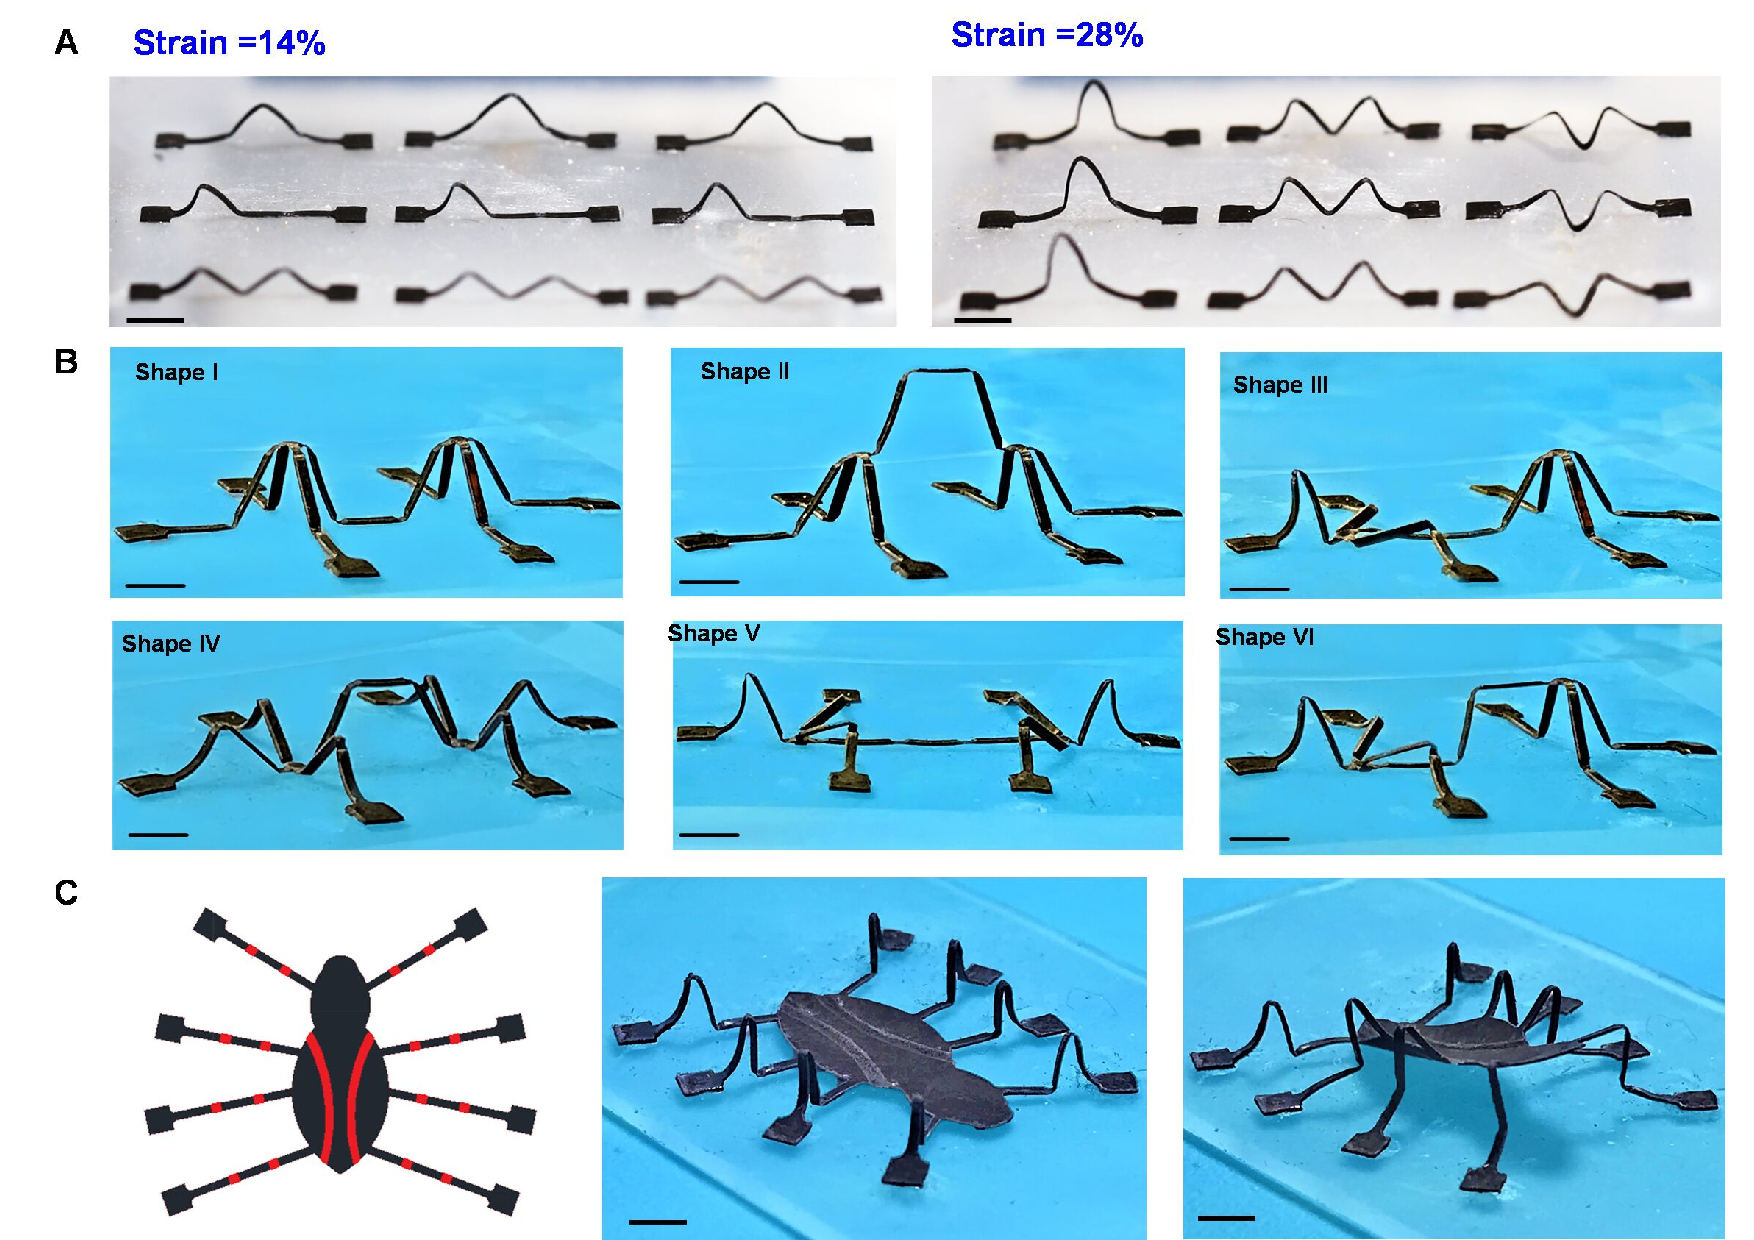
\includegraphics[width=\textwidth]{figure_4.pdf}
  \caption{
    Diverse origami-inspired, multistable ferromagnetic structures that can be actuated by magnetic forces.
    (A) An array of 3-crease ribbon structures showing different patterns formed by the multistable states of the ribbon under the strain of 14\% and 28\%, respectively.
    Scale bars, 3 mm.
    (B) Multistable states and magnetic reconfiguration of a double-table structure composed of creased ribbon segments.
    (C) A multistable biomimetic ``insect'' in its flat and standing states, respectively.
    Scale bars, 2 mm.
  }
  \label{fig:or-4}
\end{figure}



\section{Conclusion}

To sum up, it has been shown that the multistability and the associated transition paths of origami-inspired, compressively buckled ferromagnetic structures can be tailored by controlling the number of creases and assembly strain.
Our constructed phase diagram of a representative creased ribbon structure from the energy landscape analysis provides important guidelines for the targeted number of stable states by varying the two control factors.
In addition, transition pathways among the distinct stable states are computed and illustrate how the structure can be manipulated to be reconfigured along different pathways.
These have been validated using experimental results of origami-inspired ferromagnetic structures, which show targeted multistable states following designed pathways, which highly agree with modelling.

The fundamental understanding of the multistability of creased ribbon structures provides important guidelines for the design and application of multistable origami-inspired systems, with demonstrated examples including an arrays of creased ribbon units and the various states of a biomimetic ``insect'' structure.
Also, the energy landscape analysis offers an approach to study the multistable states and pathways, and can be tailored for specific applications.

These results highlight potential opportunities in the future to exploit multistable, origami-inspired ferromagnetic structures for intelligent and adaptive systems such as programmable logic array by integrating complex structure design and functional materials like stimuli-responsive polymers and electronics.
It will also be interesting to explore the concept of actively manipulating the number of stable states and their reconfiguration paths in the design of other types of functional structures by using alternative control parameters.

\begin{table}[]
  \begin{tabularx}{\textwidth}{>{\hsize=.3\hsize\linewidth=\hsize}C >{\hsize=.55\hsize\linewidth=\hsize}C >{\hsize=2.1\hsize\linewidth=\hsize}C >{\hsize=1.05\hsize\linewidth=\hsize}C}
    \hline\hline
    Topic & Symbol & Parameter description & Value \\
    \hline
    \multirow{8}{*}{\rotatebox[origin=c]{90}{Structure}}
          & $t$               & Thickness        & \SI{130}{\micro\metre} \\
          & $t_\text{crease}$ & Crease thickness & \SI{60}{\micro\metre} \\
          & $l$               & Segment length   & \SI{2.5}{\milli\metre} \\
          & $l_\text{crease}$ & Crease length    & \SI{0.8}{\milli\metre} \\
          & $w$               & Ribbon width     & \SI{0.8}{\milli\metre} \\
          & $\rho$            & Density          & \SI{2.59}{\gram\per\centi\meter\cubed} \\
          & $Y$               & Young's modulus  & \SI{1.4}{\mega\pascal} \\
          & $\nu$             & Poisson ratio    & 0.3 \\
    \hline
    \multirow{4}{*}{\rotatebox[origin=c]{90}{L-BFGS}}
          & $m$  & Iteration memory             & 5 \\
          & ---  & Initialisation iterations    & \num{30000} \\
          & ---  & Initialisation force density & \SI{10}{\newton\per\meter\squared} \\
          & ---  & Gradient RMS convergence     & $10^{-11}$ \\
    \hline
    \multirow{6}{*}{\rotatebox[origin=c]{90}{Pathways}}
          & $\alpha$ & BITSS energy constraint strength    & 10 \\
          & $\beta$  & BITSS distance constraint error     & 0.1 \\
          & $f$      & BITSS distance reduction factor     & 0.2 \\    
          & ---      & BITSS coefficient regularity        & 100 iterations \\    
          & ---      & String reparametrisation regularity & 5000 iterations \\
          & ---      & String number of images             & 60 \\
    \hline\hline
  \end{tabularx}
  \caption{\label{tab:or-params}
    Values of the parameters that are used throughout this chapter, unless otherwise specified.
  }
\end{table}

  \chapter{Conclusions and Outlook}
\label{ch:conclusion}
\graphicspath{{conclusion/fig/}}

In this thesis, we set out to apply energy landscape techniques to study complex macroscale systems, in particular multistable elastic structures. 
However, we found that traditional techniques, such as chain-of-states pathway methods, are often inadequate for these applications.
As a result, we have developed new techniques to study the energy landscapes of these large-scale systems.

In \cref{ch:bitss}, we introduced a new transition state search method, BITSS.
Unlike traditional methods, BITSS does not require any initial estimate for the pathway, making it effective for locating complex pathways without any a priori knowledge of their route.
We have shown that BITSS is compatible with adaptive remeshing techniques, which can offer simultaneous improvements to both efficiency and accuracy.
Furthermore, BITSS has been successfully applied to various challenging energy landscapes, such as where it is locally flat, or even discontinuous.
Therefore, this opens up a range of previously inaccessible problems to energy landscape analysis.

This and several other methods have then been incorporated into an energy landscape software library, `ELLib', as detailed in \cref{ch:software}.
The library is designed to be modular, flexible to use, and may be easily extended to incorporate new methods and potentials.
Additionally, it is designed to utilise parallel methods for calculating potentials, minimisation, and exploring energy landscape for large system sizes.
% However, further work is still required to ensure that some energy landscape methods can fully utilise the scalability offered by parallel computing.


Having developed this new methodology, we then applied it to investigate the behaviour of multistable buckled mesostructures.
We demonstrated in \cref{ch:mesostructures} that our approach can accurately locate stable states and reconfiguration pathways for a range of different structures, with results that match observations from experimentally manipulating the structures.
Moreover, by investigating a table structure we were able to create phase diagrams that highlight how the various states and pathways depend upon the chosen system parameters.
These findings can therefore be used to design a structure with specific functionality for a given application.

In \cref{ch:origami_ribbon} we extended our investigations to explore the effect of origami-inspired creases on the multistability of simple ribbons, which can be used as a building block for many larger structures.
Our results show that the number of creases plays a critical role in the number of available states, with three creases showing the greatest multistability, then quickly reducing to just a single stable state as the number of creases is increased further.
Furthermore, we found that increasing the strain led to changes to the available states and pathways, with a group of states that could be easily interchanged while another was separated by a large barrier.

Taken together, these results provide new insight into how the multistability of buckled mesostructures is affected by various structural and material parameters.
Our methodology and findings outline a process by which these, and other more general structures, may be tailored to obtain chosen states and reconfiguration pathways.
The identified reconfiguration pathways can also be serve as targets for remote actuation, providing a critical step towards developing rapidly reconfigurable devices for applications in soft robotics and deployable structures, among other fields.
This work has thus contributed to advancing the field of multistable elastic structures and has potential implications for a wide range of technological applications.



\section{Future work}
\subsection{Locating multiple pathways}
Many applications have multiple competing pathways between a pair of states.
For example, the snap-through buckling of a clamped beam, \cref{fig:conc-multits}(a), can take one of two asymmetric pathways.
Therefore, we may wish to use a method that enables us to locate these additional pathways.

However, locating multiple pathways between a single pair of minima is a difficult problem that has not been fully addressed by existing methods.
One possibility is to use single-ended TS search methods from the regions around each of the minima, however this is not guaranteed to find all of the TS and those that are found may not be connected to the states of interest.
Another approach is to make initial guesses using a chain-of-states method, but this requires some knowledge of the expected pathways and the initial interpolation may be difficult.
Alternatives are possible, such as transition path sampling \cite{Bolhuis2002} or using molecular dynamics over long time-scales, but these can be very computationally costly.

\begin{figure}[htb]
  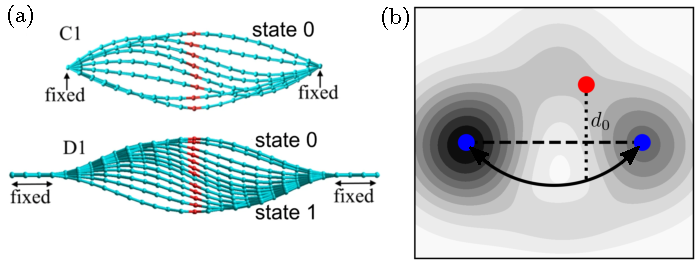
\includegraphics{multits.pdf}
  \caption{
    (a) The asymmetric snap-through buckling pathways for constrained thin sheets (specifically graphene membranes).
    The endpoints are allowed to rotate in the first, and they are fixed in the second.
    An equivalent, reflected pathway is possible in both.
    Adapted with permission from \cite{Yamaletdinov2018}.
    (b) Schematic illustrating a 2D landscape with two pathways, and a possible modified distance metric that would enable BITSS to locate the second TS.
    The pathway's radius of curvature is calculated to set a certain distance $d_0$ from the known TS (red dot).
  }
  \label{fig:conc-multits}
\end{figure}

One possibility would be to extend the BITSS method to locate multiple TS by modifying the distance metric.
Taking inspiration from general relativity, in which mass can curve space-time and reduce the distance between two points, once BITSS has located a TS a ``negative mass'' could be applied, effectively expanding space around that point.
This would result in the two states attempting to move away from the known TS as they converge, and hopefully converging to another.
This could then be repeated to find multiple different transition states that separate the two minima.
Such a method would bear a resemblance to the deflated Newton method\cite{Noack2017}, but for finding multiple TS instead of minima.

Of course attempting to calculate an accurate distance based upon a curved space-time would be exceedingly complicated, however it does provide a useful analogy.
Instead, a simpler approach could be to consider a circular arc between the states that has a radius of curvature that points it away from the TS so that the images would converge a chosen distance away, as illustrated in \cref{fig:conc-multits}(b).
By repeating BITSS and continually increasing this distance bias, it could be possible to locate all available pathways.


\subsection{3D elastic metamaterials}
In this thesis, we have investigated the behavior of two-dimensional elastic structures through the use of a discretised shell model that is particularly effective in analyzing the bending of thin films.
However, this approach is insufficient for studying a variety of complex reconfigurable structures such as three-dimensional mechanical metamaterials, as discussed in \cref{sec:es-metamaterials}.
As a result, a natural extension to our work would be to incorporate a three-dimensional elastic potential, such as one based on the finite element method, to better examine these systems.

Energy landscape analysis could be a promising tool for addressing a wide range of problems associated with mechanical metamaterials.
For example, the effectiveness of collisional energy-absorbing structures\cite{Shan2015,Giri2021} is heavily influenced by material and geometric factors, which modify the energy barriers of the various reconfiguration pathways.
Therefore, by optimising the barriers as we demonstrated in \cref{sec:ell-demo}, we could gain valuable insights into how to maximize the efficiency of these structures.

A similar analysis could be applied to flexible metamaterials that undergo a large-scale, bistable transformation, which are of interest to develop deployable structures \cite{Shang2018,Zareei2020}.
Here, an important consideration is their durability, i.e. how many times they can be reconfigured without breaking, which is found to be inversely correlated with the elastic strain energy during the transition \cite{Shang2018}.
In this case, investigating the minimum energy pathway could provide the structural parameters that minimise the energy barrier, thereby increasing durability, while allowing the structure to remain bistable.

\begin{figure}
  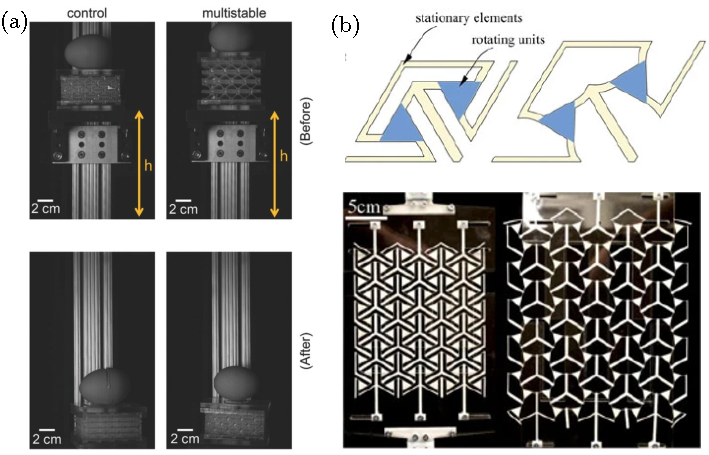
\includegraphics{metamaterials.pdf}
  \caption{
    (a) Energy absorbing structures.
    Adapted with permission from \cite{Shan2015}.
    (b) Bistable auxetic metamaterial that undergoes a transition to a deployed state.
    Adapted with permission from \cite{Shang2018}.
  }
\end{figure}


\subsection{Reconfigurable surface structures for adaptable wetting}
An interesting application of the creased ribbon structures investigated in \cref{ch:origami_ribbon} could be to create an array of adaptable surface structures that could be remotely switched between two states in order to alter the wetting properties of a surface.

For example, it is known that an array of pillars on a surface can keep a droplet in a suspended Cassie--Baxter state where it can exhibit superhydrophobic behaviour.
But this depends upon the geometry of the posts, and if they are further apart the droplet may instead transition to a Wenzel state, sinking into the structure and losing the superhydrophobic behaviour.
These two states could potentially be switched from one to the other using the structure in \cref{fig:conc-wetting}(b), which has one state where the `pillars' are larger with less spacing between then, and another state with smaller pillars and larger spacing.

However, due to their more complicated design, flexible ribbon structures would restricted to larger sizes than a simple pillar geometry, making the Wenzel state more prone to failure.
Energy landscape methods could be used to address this using a similar analysis as performed in \cite{Panter2019a}.
This would provide information as to how the structure should be modified to maximise the energy barrier that prevents the droplet from penetrating the structure.

\begin{figure}
  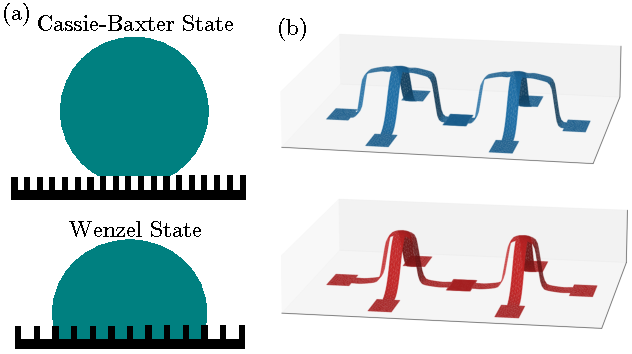
\includegraphics{wetting.pdf}
  \caption{
    (a) Illustration of the Cassie--Baxter and Wenzel states of a droplet on a structured surface.
    (b) An origami-inspired mesostructure with two states that could be used to realise an adaptable wetting surface.
  }
  \label{fig:conc-wetting}
\end{figure}


  \appendix
  \let\cleardoublepage\clearpage
  \chapter{Supplementary Material}\label{ch:appendix}

Supplementary material for this thesis can be found at this link: \url{https://doi.org/10.15128/r1n870zq87j}

This contains the ELLib software library, the script used to perform the structural optimisation in \cref{sec:ell-demo}, and supplementary videos for \cref{ch:mesostructures,ch:origami_ribbon}, which are described below.
\\


\begingroup
\captionsetup{type=video}

\caption{Reconfiguration path 1 for a table structure with $L = \SI{1.04}{\milli\meter}$.}
\label{vid:pathA1}

\caption{Reconfiguration path 2 for a table structure with $L = \SI{1.04}{\milli\meter}$.}
\label{vid:pathA2}

\caption{Reconfiguration path 1 for a table structure with $L = \SI{0.8}{\milli\meter}$.}
\label{vid:pathB1}

\caption{Reconfiguration path 2* for a table structure with $L = \SI{0.8}{\milli\meter}$.}
\label{vid:pathB2}

\caption{Reconfiguration path 1 for a table structure with $L = \SI{0.72}{\milli\meter}$.}
\label{vid:pathC1}


\caption{Progression of the five regimes of the 3-crease ribbon when the strain is increased from 0\% to 40\%, with a magnetic reconfiguration among the stable states in each regime.}
\label{vid:ribbon-progress}

\caption{The single pathway (P\textsubscript{1-2}) for a 3-crease ribbon at 8\% strain.}
\label{vid:ribbon8}

\caption{The three pathways (P\textsubscript{1-2}, P\textsubscript{1-3}, and P\textsubscript{2-3}) for a 3-crease ribbon at 14\% strain.}
\label{vid:ribbon14}

\caption{The two pathways (P\textsubscript{1-2*-3} and P\textsubscript{1-3}) for a 3-crease ribbon at 18\% strain.}
\label{vid:ribbon18}

\caption{The three pathways (P\textsubscript{1-2*-3}, P\textsubscript{1-3}, and P\textsubscript{3-4}) for a 3-crease ribbon at 24\% strain.}
\label{vid:ribbon24}

\caption{The two pathways (P\textsubscript{1-2*-4} and P\textsubscript{1-3*-4}) for a 3-crease ribbon at 34\% strain.}
\label{vid:ribbon34}

\endgroup


  \bibliographystyle{unsrt}
  \addcontentsline{toc}{chapter}{Bibliography}
  \singlespacing
  \bibliography{library.bib}

\end{document}
